% cd /disks/PROJECT/Mickael/COMMUNICATION/BeamerThesis/;
% pdflatex BeamerThesis.tex; bibtex BeamerThesis; pdflatex BeamerThesis.tex; pdflatex BeamerThesis.tex
% evince BeamerThesis.pdf &

\documentclass[10pt,  xcolors={RGB}, hyperref={%
    pdfpagelabels=false,
    colorlinks=true,
    pdftex=true,
    bookmarks=true,
    bookmarksopen=true,
    hyperfootnotes=true}]{beamer}
\pdfpageattr{/Group << /S /Transparency /I true /CS /DeviceRGB>>}

\usepackage[T1]{fontenc}
\usepackage[utf8]{inputenc}
\usepackage{graphicx}
\usepackage{tabularx}
\usepackage{array}
\usepackage{multirow}
\usepackage{pifont}
\usepackage{multicol}

\usepackage{marvosym}

\usepackage[english, francais]{babel}
\selectlanguage{francais}
\frenchbsetup{StandardLists=true}
\DecimalMathComma

\usepackage{etoolbox}
\makeatletter
    \let\BEAMER@footnotetext\@footnotetext
\makeatother
\usepackage{setspace}
\makeatletter
    % restore the meaning of \@footnotetext
    \let\@footnotetext\BEAMER@footnotetext
    % patch the relevant command to do single spacing in footnotes
    \expandafter\patchcmd\csname beamerx@\string\beamer@framefootnotetext\endcsname
        {\reset@font}
        {\def\baselinestretch{\setspace@singlespace}\reset@font}
        {}{}
\makeatother

\usepackage[sfdefault]{AlegreyaSans}
\renewcommand{\familydefault}{\sfdefault}

\usepackage[square, authoryear]{natbib}

\usepackage[format=plain, font=scriptsize, labelfont=bf, hang]{caption} % Required for specifying captions to tables and figures
\usepackage{enumitem}

%-------------- Define Colours ------------------%
\definecolor{dodgerblue}{RGB}{30,144,255}
\definecolor{springgreen3}{RGB}{0,139,69}
\definecolor{springgreen2}{RGB}{0,205,102}
\definecolor{firebrick2}{RGB}{238,44,44}
\definecolor{maroon2}{RGB}{238,48,167}
\definecolor{goldenrod2}{RGB}{238,180,34}
\definecolor{deepskyblue}{RGB}{0,191,255}

\definecolor{T2D}{RGB}{255,100,255}
\definecolor{FG}{RGB}{0,170,69}
\definecolor{FI}{RGB}{0,138,139}
\definecolor{FP}{RGB}{0,173,247}
\definecolor{2hGlu}{RGB}{255,73,73}
\definecolor{HbA1c}{RGB}{198,162,7}
\definecolor{CIR}{RGB}{253,141,48}
\definecolor{1hGlu}{RGB}{180,110,253}



%-------------- Customise template --------------%
\usetheme{CambridgeUS}
\useoutertheme{infolines}
\useinnertheme{rectangles}
\setbeamercolor{frametitle}{fg=white, bg=springgreen3!90!black!60!white}
\setbeamercolor{title}{fg=white, bg=springgreen3!50!white}
\setbeamercolor{palette primary}{fg=springgreen3!40!black, bg=springgreen3!50!white}
\setbeamercolor{palette secondary}{fg=springgreen3!30!black, bg=springgreen3!70!white}
\setbeamercolor{palette tertiary}{fg=springgreen3!20!black, bg=springgreen3!90!white}
\setbeamercolor{structure}{fg=springgreen3!70!white}
\setbeamercolor{background canvas}{bg=white}
\setbeamercolor{normal text}{fg=black}
\setbeamercolor{block title}{bg=dodgerblue, fg=white}
\setbeamercolor{example text}{fg=springgreen3}
\setbeamercolor{block title example}{bg=springgreen3, fg=white}
\setbeamercolor{alerted text}{fg=firebrick2}
\setbeamercolor{block title alerted}{bg=firebrick2, fg=white}
\setbeamertemplate{navigation symbols}{}
\addtobeamertemplate{headline}{\hypersetup{allcolors=black}}{}

\setbeamerfont{frametitle}{series=\slshape\bfseries}
\setbeamerfont{framesubtitle}{series=\slshape\bfseries\textit}
\setbeamerfont{section title}{series=\slshape\bfseries}


%-------------- Define Title Page ---------------%
\def\cst#1{\def\@cst{#1}}
\defbeamertemplate*{title page}{custom}[1][]{
    \renewcommand{\baselinestretch}{1.25}
    \begin{centering}
        \begin{beamercolorbox}[sep=3pt,center,#1]{institute}
            \usebeamerfont{institute}{\insertinstitute}
        \end{beamercolorbox}
        \vfill
        \begin{beamercolorbox}[sep=8pt, center, colsep=-4bp, rounded=true, shadow=true, #1]{title}
            \usebeamerfont{title}\inserttitle\par%
            \ifx\insertsubtitle\@empty%
            \else%
            \vskip0.25em%
            {\usebeamerfont{subtitle}\usebeamercolor[fg]{subtitle}\insertsubtitle\par}%
            \fi%
        \end{beamercolorbox}%
        \vskip1em\par
        \begin{beamercolorbox}[sep=8pt,center,#1]{author}
            \usebeamerfont{author}\insertauthor
        \end{beamercolorbox}
        \begin{beamercolorbox}[sep=8pt,center,#1]{}
            \usebeamerfont{institute}\@cst
        \end{beamercolorbox}
        \begin{beamercolorbox}[sep=8pt,center,#1]{date}
            \usebeamerfont{date}{\small\insertdate}
        \end{beamercolorbox}
        \vfill
        {\usebeamercolor[fg]{titlegraphic}\inserttitlegraphic\par}
    \end{centering}
    \renewcommand{\baselinestretch}{1.5}
}



\hypersetup{%
    linkcolor=dodgerblue,
    urlcolor=firebrick2,
    citecolor=springgreen3,
    filecolor=goldenrod2,
    menucolor=dodgerblue
}
%\renewcommand{\thefootnote}{\textcolor{maroon2}{\arabic{footnote}}}

\usepackage{textcomp}

\newcommand\bref[2]{\hyperref[#1]{#2~\ref*{#1}}}
\newcommand\cmd[1]{\texttt{\color{black}\textbf{#1}}}
\newcommand\cmdb[1]{\texttt{\color{dodgerblue}\textbf{#1}}}
\newcommand\cmdr[1]{\texttt{\color{firebrick2}\textbf{#1}}}
\newcommand\cmdg[1]{\texttt{\color{springgreen3}\textbf{#1}}}
\newcommand\cmdy[1]{\texttt{\color{goldenrod2}\textbf{#1}}}
\newcommand\blue[1]{{\color{dodgerblue}\textbf{#1}}}
\newcommand\red[1]{{\color{firebrick2}\textbf{#1}}}
\newcommand\green[1]{{\color{springgreen3}\textbf{#1}}}
\newcommand\yellow[1]{{\color{goldenrod2}\textbf{#1}}}
\newcommand\pql{{\rmfamily \textbf{\color{goldenrod2}``}}}
\newcommand\pqr{{\rmfamily \textbf{\color{goldenrod2}''}}}
\newcommand\pq[3]{{\rmfamily \textbf{\color{#3}``}}#1{\rmfamily \textbf{\color{#3}''}} - \textcolor{#3}{#2}}
\newenvironment{bquote}[1]
    {\begin{quotation}
    \vspace{10pt}
    \newcommand{\bqauthor}{\normalfont \begin{quote}\begin{flushright}--- #1\end{flushright}\end{quote}}
    \rmfamily \itshape {\huge\textbf{``}}
    }
    {{\huge\textbf{''}}
    \bqauthor
    \end{quotation}
    }


\let\oldcitep=\citep
\renewcommand{\citep}[1]{\green{\oldcitep{#1}}}
\let\oldcitet=\citet
\renewcommand{\citet}[1]{\green{\oldcitet{#1}}}
\let\oldcite=\cite
\renewcommand{\cite}[1]{\green{\oldcite{#1}}}

\newcommand\lettrine[1]{{\huge{$\mathcal{#1}$}}}


\usepackage{listings}

\usepackage{ifxetex,ifluatex}
\newif\ifsecpart
\AtBeginSection{
    \ifsecpart
    \else
        \let\insertsectionnumber\relax
        \let\sectionname\relax
        \frame{\sectionpage}\note{}
    \fi
}

\everymath{\color{dodgerblue}}
% \everydisplay{\color{springgreen3}}

%-------------- Define Title Page Variables ---------------%
\date[{\color{black}29 Septembre 2017}]{{\color{springgreen3!90!white}29 Septembre 2017}}
\author[{\color{black}\textsc{Mickaël CANOUIL}}]{%
    \texorpdfstring{{\itshape\color{springgreen3!90!white}\textbf{Soutenance de Thèse}}\\\itshape\textsc{Mickaël CANOUIL\\ \vskip -0.25cm
    \href{mailto:mickael.canouil@cnrs.fr}{{\scriptsize mickael.canouil@cnrs.fr}}}}{\itshape\textsc{Mickaël CANOUIL}}
}
\institute[CNRS UMR 8199]{%
    \color{springgreen3!90!white}\blue{G}énomique \blue{I}ntégrative et \blue{M}odélisation des \blue{M}aladies \blue{M}étaboliques
    \linebreak UMR 8199 (CNRS / Université de Lille 2 / Institut Pasteur de Lille)%
}
\titlegraphic{%
    
\includegraphics[height=1cm, keepaspectratio]{template/logo_cnrs.pdf}\hspace{1.5cm}
    
\includegraphics[height=1cm, keepaspectratio]{template/UL2-WEB-2014.png}\hspace{1.5cm}
    
\includegraphics[height=1cm, keepaspectratio]{template/Institut-Pasteur-de-Lille.png}\hspace{1.5cm}
    
\includegraphics[height=1cm, keepaspectratio]{template/logo_egid.pdf}%
}
\title[\texorpdfstring{\color{black}\slshape{Soutenance de Thèse}}{}]{%
    \slshape\bfseries{Développement et Application de Méthodologies Statistiques pour Études Multi-Omiques dans le Diabète de Type 2}%
}
\subtitle{\slshape\bfseries\textit{Au-delà de l'Ère des Études d'Association Pangénomiques}}
\cst{{\itshape\color{springgreen3!90!white}\textbf{Direction de Thèse}}\\ Dr. Ghislain Rocheleau \& Pr. Philippe Froguel}


\usepackage{tikz}
\usebackgroundtemplate{%
    \shorthandoff{;}%
    \tikz\node[opacity=0.1, inner sep=0pt] {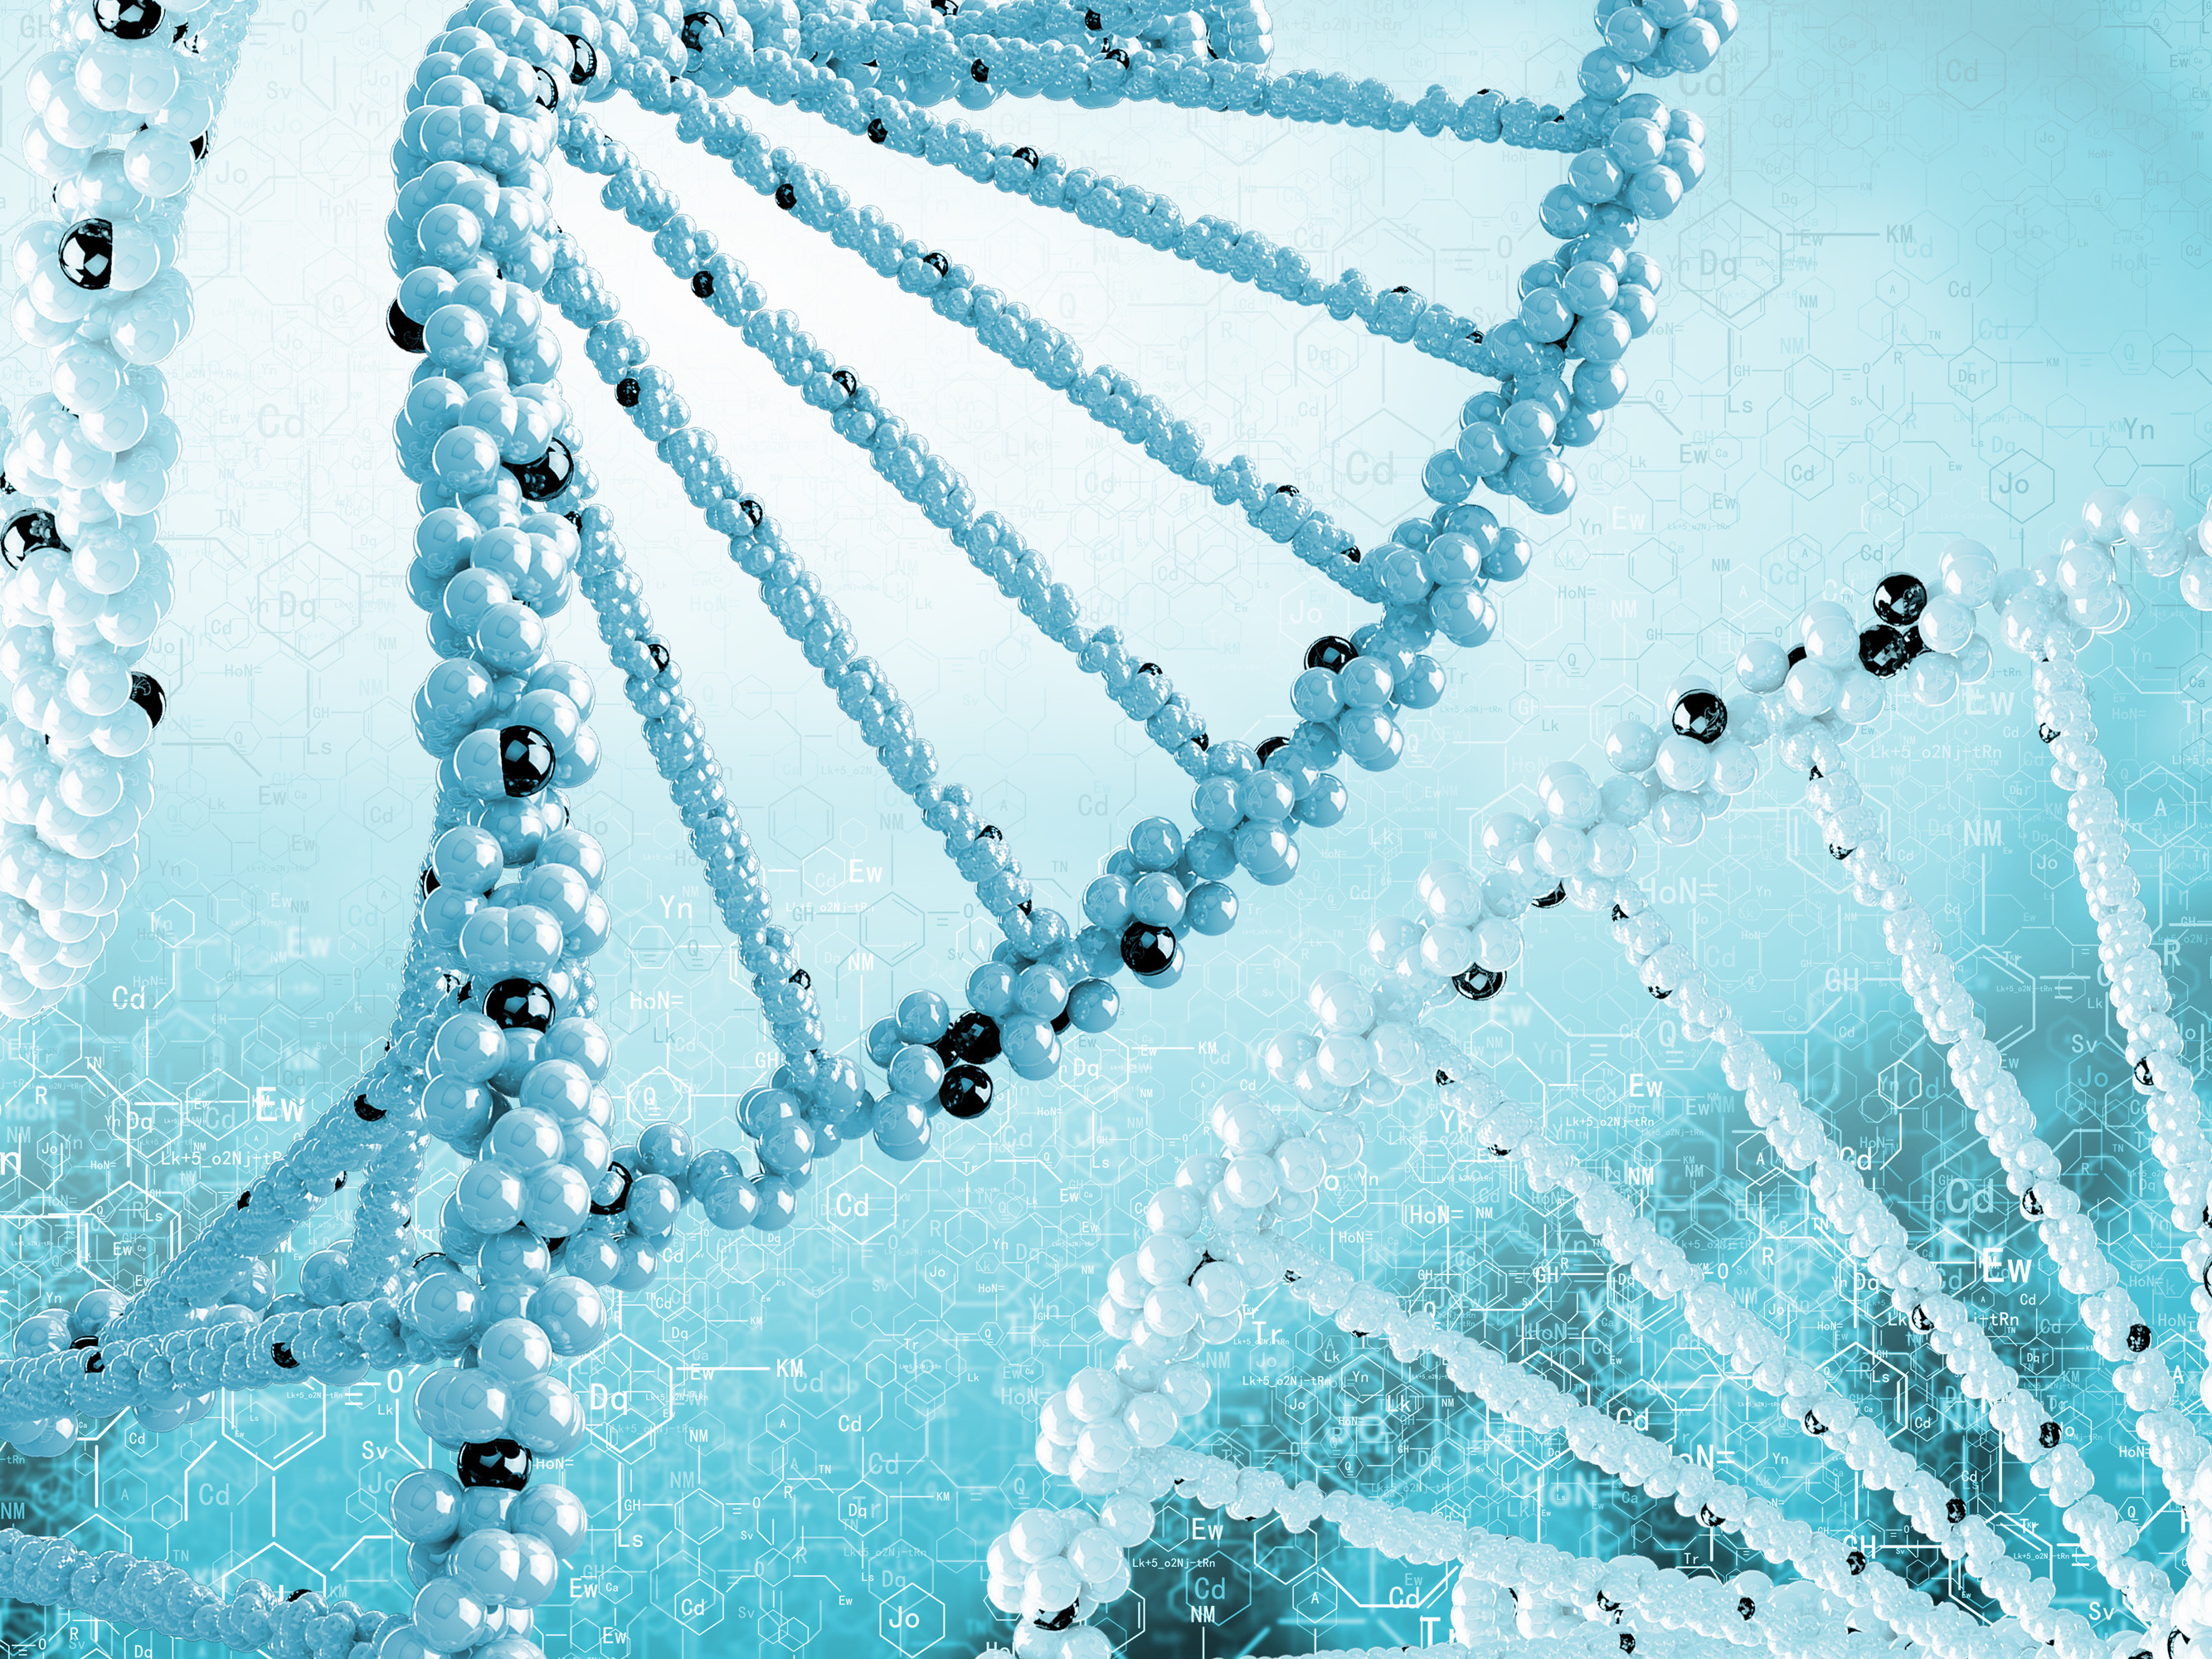
\includegraphics[height=\paperheight, width=\paperwidth]{template/BG03_Beamer.jpg}};%
}

%\AtBeginNote{\hspace*{-0.75cm}\addtolength\leftmargini{-0.75cm}}
%\AtEndNote{\addtolength\leftmargini{0.75cm}}
\makeatletter
    \defbeamertemplate{note page}{infolines}
    {%
        {%
            \scriptsize
            \insertvrule{.25\paperheight}{white!90!black}
            \vskip-.25\paperheight
            \nointerlineskip
            \vbox{
                \hfill\insertslideintonotes{0.25}\hskip-\Gm@rmargin\hskip0pt%
                \vskip-0.25\paperheight%
                \nointerlineskip
                \begin{pgfpicture}{0cm}{0cm}{0cm}{0cm}
                    \begin{pgflowlevelscope}{\pgftransformrotate{90}}
                        {\pgftransformshift{\pgfpoint{-2cm}{0.2cm}}%
                            % \pgftext[base,left]{\footnotesize\the\year-\ifnum\month<10\relax0\fi\the\month-\ifnum\day<10\relax0\fi\the\day}}
                            \pgftext[base,left]{\footnotesize 2017-09-29}}
                    \end{pgflowlevelscope}
                \end{pgfpicture}%
            }
            \nointerlineskip
            \vbox to .25\paperheight{\vskip0.5em
                \hbox{\insertshorttitle[width=8cm]}%
                \setbox\beamer@tempbox=\hbox{\insertsection}%
                \hbox{\ifdim\wd\beamer@tempbox>1pt{\hskip4pt\raise3pt\hbox{\vrule width0.4pt height7pt\vrule width 9pt height0.4pt}}\hskip1pt\hbox{\begin{minipage}[t]{7.5cm}\def\breakhere{}\insertsection\end{minipage}}\fi}%
                \setbox\beamer@tempbox=\hbox{\insertsubsection}%
                \hbox{\ifdim\wd\beamer@tempbox>1pt{\hskip17.4pt\raise3pt\hbox{\vrule width0.4pt height7pt\vrule width 9pt height0.4pt}}\hskip1pt\hbox{\begin{minipage}[t]{7.5cm}\def\breakhere{}\insertsubsection\end{minipage}}\fi}%
                \setbox\beamer@tempbox=\hbox{\insertshortframetitle}%
                \hbox{\ifdim\wd\beamer@tempbox>1pt{\hskip30.8pt\raise3pt\hbox{\vrule width0.4pt height7pt\vrule width 9pt height0.4pt}}\hskip1pt\hbox{\insertshortframetitle[width=7cm]}\fi}%
                \vfil
            }%
        }%
        \vskip.25em
        \nointerlineskip
        \hspace*{-0.75cm}
        \begin{minipage}{\columnwidth} % this is an addition
        	 \addtolength\leftmargini{-0.5cm}
        	 \setstretch{1}
            {\textcolor{black}{\scriptsize\insertnote}}
            \addtolength\leftmargini{0.5cm}
        \end{minipage} % this is an addition
    }
\makeatother
\setbeamertemplate{note page}[infolines]
% \setbeamertemplate{note page}[plain]

\usepackage{pgfpages}
%\setbeameroption{show notes on second screen=right}


\renewcommand{\footnotesize}{\tiny}

\captionsetup{labelformat=empty, textfont={bf,it}, width=5cm}

\renewcommand{\baselinestretch}{1.5}


\setitemize{label=\usebeamerfont*{itemize item}%
\usebeamercolor[fg]{itemize item}
\usebeamertemplate{itemize item}}

\setlist[description]{font={\bfseries\sffamily\color{springgreen3}}}

\def\Put(#1,#2)#3{\leavevmode\makebox(0,0){\put(#1,#2){#3}}}


\setbeameroption{hide notes} % \setbeameroption{hide notes}
\begin{document}
\maketitle
\note{}


\begin{frame}{Sommaire}
    \vspace{-3em}
    \begin{multicols}{2}
        \noindent
        \tableofcontents[sectionstyle=show/show, subsectionstyle=hide/hide/hide, subsubsectionstyle=hide/hide/hide, sections={1-2}]
        \columnbreak
        \tableofcontents[sectionstyle=show/show, subsectionstyle=hide/hide/hide, subsubsectionstyle=hide/hide/hide, sections={3-4}]
    \end{multicols}
\end{frame}


%########################
\section{Contexte}
\subsection{Le Diabète dans le Monde}
\begin{frame}{\subsecname}
    \par{Quelques chiffres sur le diabète \citep{roglic_global_2016}:}
    \vspace{1em}

    \begin{minipage}[t]{0.475\columnwidth}
        \vspace{2em}
        \begin{center}
        \par{\textbf{En 1980}}
        \begin{itemize}
            \item \green{\texttildelow 108 millions} de diabétiques
            \item prévalence mondiale de \green{4,7 \%}
        \end{itemize}
        \end{center}
        \vspace{2em}
    \end{minipage}%
    \hfill\alt<2>{\vline}{}\hfill
    \begin{minipage}[t]{0.475\columnwidth}%
        \vspace{2em}
        \begin{center}
        \par{\alt<2>{\textbf{En 2014}}{}}
        \begin{itemize}
            \item<2> \green{\texttildelow 400 millions} de diabétiques
            \item<2> prévalence mondiale de \green{8,5 \%}
        \end{itemize}
        \end{center}
        \vspace{2em}
    \end{minipage}
\end{frame}


\subsection{Les Formes de Diabète}
\begin{frame}{\subsecname}
    \par{Principalement deux formes de diabète:}
    \begin{description}
        \setlength{\itemindent}{0.25in}
        \item[Diabète de type 1] Maladie auto-immune (diabète ``jeune'')
        \item[{\textcolor<2>{dodgerblue}{\textbf<2>{Diabète de type 2}}}] {\textcolor<2>{dodgerblue}{\textbf<2>{Maladie métabolique complexe (diabète ``adulte'')}}}
    \end{description}
\end{frame}


\subsection{Le Diabète de Type 2}
\begin{frame}{\subsecname}
    \par{Le \green{diabète de type 2} (T2D) se caractérise par une \green{hyperglycémie} chronique, conséquence d'une production insuffisante d'\green{insuline}, et est défini selon deux critères de diagnostique:}

    \vspace{-1em}
    \begin{minipage}[t]{0.475\columnwidth}
        \vspace{1em}
        {\small
        \begin{description}\setlength{\itemsep}{1.5em}
            \item[OMS] \textit{Organisation Mondiale de la Santé}\\
                \begin{itemize}\setlength{\itemindent}{-0.25in}\vspace{-1.5em}
                    \item $[\textrm{Glycémie}_{\textrm{à jeun}}] \geq 7\ {\textrm{mmol/L}}$
                    \item $[\textrm{Glycémie}_{\textrm{à 2 heures}}] \geq 11,1\ {\textrm{mmol/L}}$
                \end{itemize}
            \item[ADA] \textit{Association Américaine pour le Diabète}\\
                \begin{itemize}\setlength{\itemindent}{-0.25in}\vspace{-1.5em}
                    \item $[\textrm{Glycémie}_{\textrm{à jeun}}] \geq 7\ {\textrm{mmol/L}}$
                    \item $[\textrm{HbA1c}] > 6,5\ \%$
                \end{itemize}
        \end{description}
        }
        \vspace{1em}
    \end{minipage}%
    \hfill\vline\hfill
    \begin{minipage}[t]{0.475\columnwidth}%
    \vspace{2em}
        \begin{center}
            \fbox{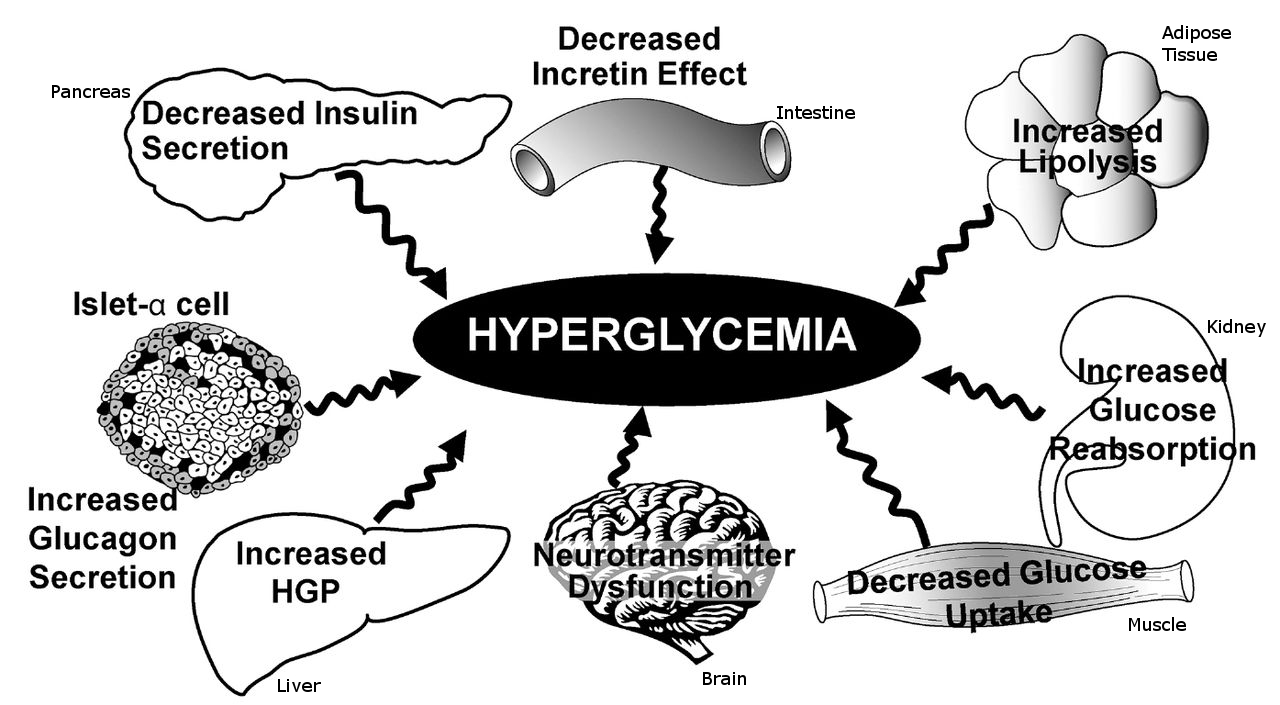
\includegraphics[width=5cm]{images/hyperglycemia_t2d.jpg}}
            \captionof{figure}{\color{springgreen3}Tissus et organes impliqués dans l'hyperglycémie et le diabète de type 2 (HGP: ``hepatic glucose production'', production hépatique de glucose).}
        \end{center}
    \vspace{1em}
    \end{minipage}
\end{frame}


\subsection{La Génétique du Diabète de Type 2}
\begin{frame}{\subsecname}
	\begin{minipage}[c]{0.635\textwidth}
		\vspace{1em}
			{\color{black}\fbox{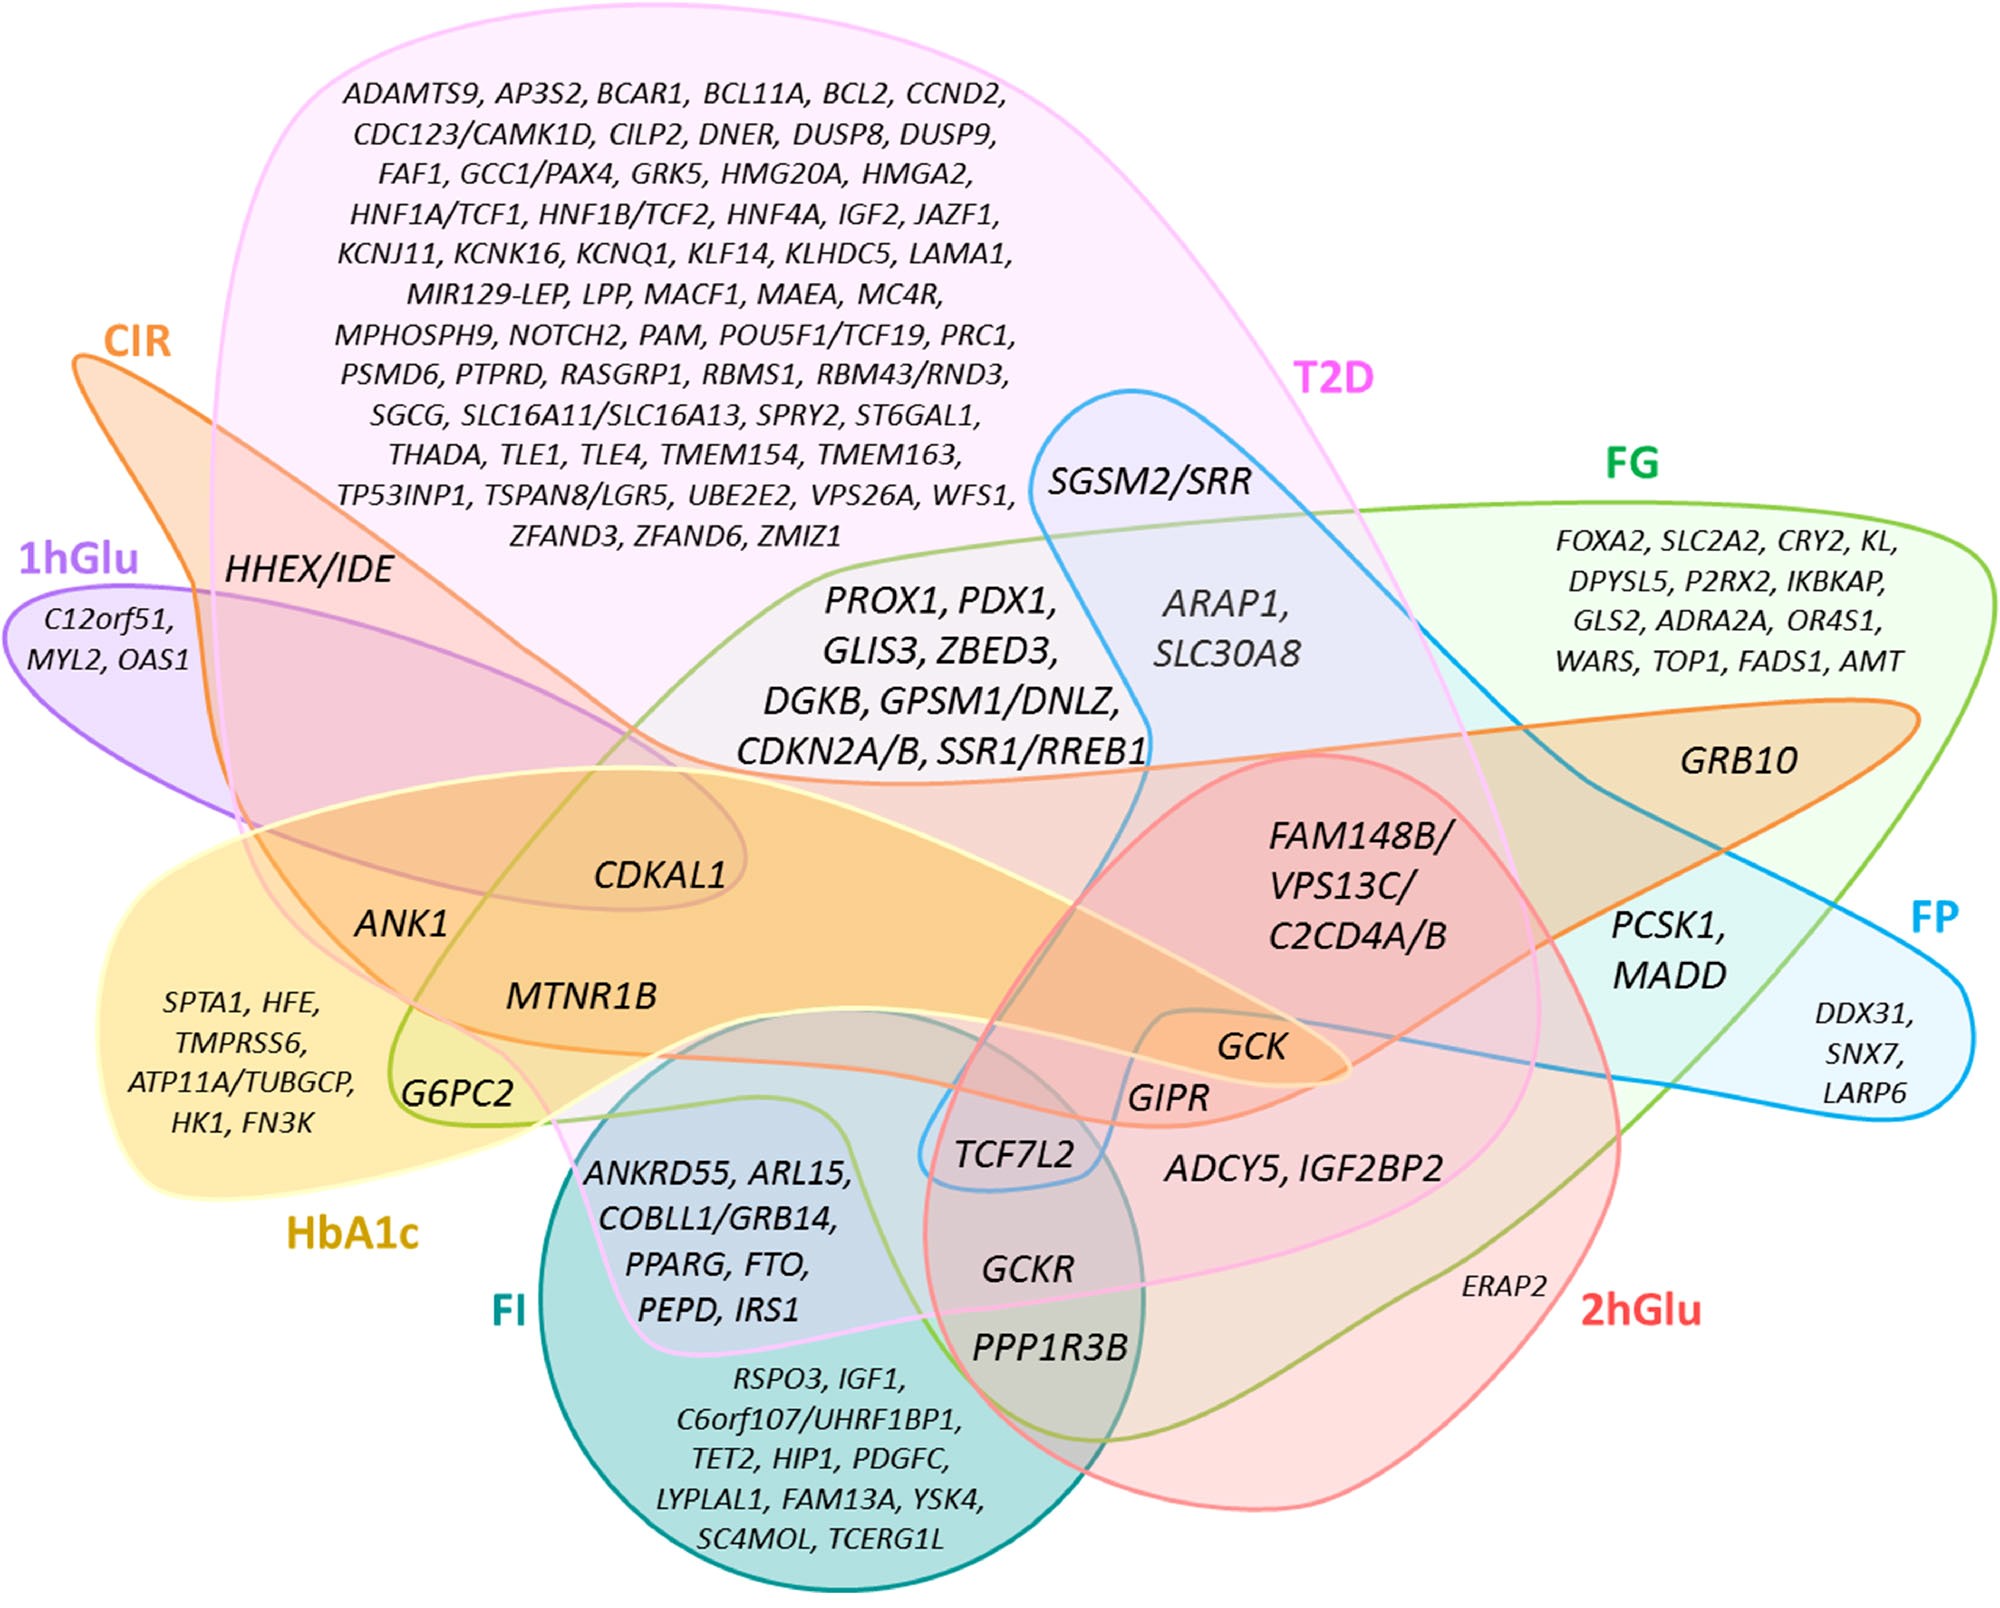
\includegraphics[width=7cm]{images/ProkopenkoMetaboDiagram.png}}}
		\vspace{1em}
	 \end{minipage}
	 \hfill
	 \begin{minipage}[c]{0.36\textwidth}
		\vspace{1em}
		\captionsetup{labelformat=empty, textfont={bf,it}, width=\textwidth}
		\captionof{figure}{\color{springgreen3}Diagramme de Venn des loci identifiés par études d'association pangénomiques pour leur effet sur différents traits glycémiques et le diabète de type 2 \citep{marullo_insights_2014}.\\[1em]
\textcolor{T2D}{T2D: diabète de type 2;}\\
\textcolor{FG}{FG: glycémie à jeun;}\\
\textcolor{FI}{FI: insulinémie à jeun;}\\
\textcolor{FP}{FP: proinsulinémie à jeun;}\\
\textcolor{2hGlu}{2hGlu: glycémie à 2 heures;}\\
\textcolor{1hGlu}{1hGlu: glycémie à 1 heure;}\\
\textcolor{HbA1c}{HbA1c: hémoglobine glyquée;}\\
\textcolor{CIR}{CIR: ratio carbohydrate-insuline.}
}
		\vspace{1em}
	\end{minipage}
\end{frame}


\subsection{Un Grand Nombre de Découverte, mais ...}
\begin{frame}{\subsecname}
    \par{Plus de \green{100 loci identifiés}, mais:}

    \vspace{-1em}
    \begin{minipage}[t]{0.475\columnwidth}
        \vspace{1em}
        \begin{center}
            {\color{black}\fbox{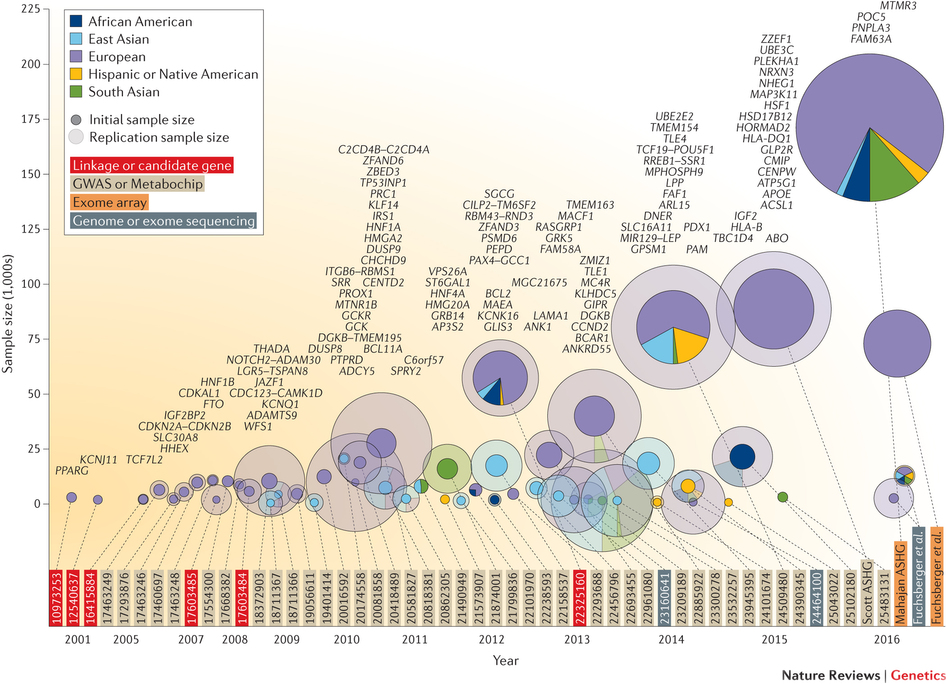
\includegraphics[width=5cm]{images/T2Dhistory.jpg}}}
            \captionof{figure}{\color{springgreen3}Historique des loci de susceptibilité au diabète de type 2 identifiés par études d'association pangénomiques \citep{flannick_type_2016}.}
        \end{center}
        \vspace{1em}
    \end{minipage}%
    \hfill\vline\hfill
    \begin{minipage}[t]{0.475\columnwidth}%
        \vspace{1em}
        {\small
            \begin{itemize}
                \item des \green{effets} sur la glycémie à jeun (FG) et le risque de diabète de type 2 (T2D) \green{\mbox{peu corrélés}}\vspace{-0.5em}
                \item<2>[$\Rightarrow$] Effet génétique conjoint sur \green{FG} et le risque de \green{T2D}?
                \item une \green{fonction} biologique \green{méconnue} ou \mbox{inconnue} pour la plupart\vspace{-0.5em}
                \item<2>[$\Rightarrow$] Lien entre l'\green{expression} des gènes et la \mbox{sécrétion} d'\green{insuline}?
            \end{itemize}
        }
        \vspace{1em}
    \end{minipage}
\end{frame}


%########################
\section{Glycémie et Diabète de Type 2: un Effet Génétique Conjoint?}


\begin{frame}{\secname}
\begin{center}
 \fcolorbox{black}{white}{
 \begin{minipage}[t]{0.85\columnwidth}\setstretch{1}
 {\normalsize \slshape\bfseries{Variants Génétiques Associés à la Trajectoire de la Glycémie à Jeun et à l'Incidence du Diabète de Type 2 : Une Approche par Modèle Joint}}\\[0.5em]
{\tiny \textbf{Mickaël Canouil}\textsuperscript{1,2,3}, Beverley
Balkau\textsuperscript{4,5,6}, Ronan Roussel\textsuperscript{7,8,9},
Philippe Froguel\textsuperscript{1,2,3,10} \& Ghislain
Rocheleau\textsuperscript{1,2,3}}
\end{minipage}%
}
\end{center}
\end{frame}


\subsection{Contexte \& Objectifs}
\begin{frame}{\subsecname}
    \vspace{-1.5em}
    \begin{minipage}[t]{0.475\columnwidth}
        \vspace{0.5em}
        {\scriptsize
            \begin{center}
                \setstretch{0.75}
                \par{``In all cases, the glucose-raising allele was associated with increased risk of T2D, yet fasting glucose effect sizes and T2D ORs were weakly correlated''}
            \end{center}
        }
        \begin{center}
            {\color{black}\fbox{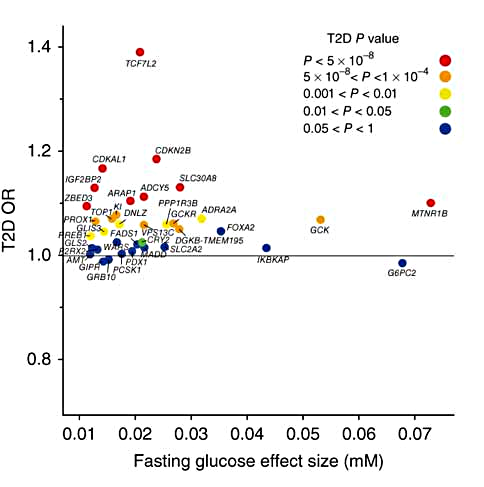
\includegraphics[width=4cm]{images/ng2385-F2.png}}}
            \captionof{figure}{\color{springgreen3}Taille d'effet $\textcolor{springgreen3}{\beta}$ et Odd Ratio respectivement pour l'augmentation de la concentration de glucose et du risque de T2D (\mbox{\citet{scott_large-scale_2012}}).}
        \end{center}
        \vspace{0.5em}
    \end{minipage}
    \hfill\vline\hfill
    \begin{minipage}[t]{0.475\columnwidth}
        \vspace{3em}
        {\small
            \begin{center}
                \begin{description}
                    \item[Objectif] \ \\Recherche de variants (SNPs) associés à la fois à la glycémie à jeun et au diabète de type 2
                    \item[Données] \ \\Cohorte D.E.S.I.R.
                    \item[Méthode] \ \\Modèle Joint
                \end{description}
            \end{center}
        }
        \vspace{1em}
    \end{minipage}
\end{frame}


\subsection{Modèle Joint}
\subsubsection{Présentation}
\begin{frame}{\subsecname: \subsubsecname}
    \vspace{-1em}
    \begin{minipage}[t]{0.475\columnwidth}
            \vspace{4em}
        \begin{center}
            {\color{black}\fbox{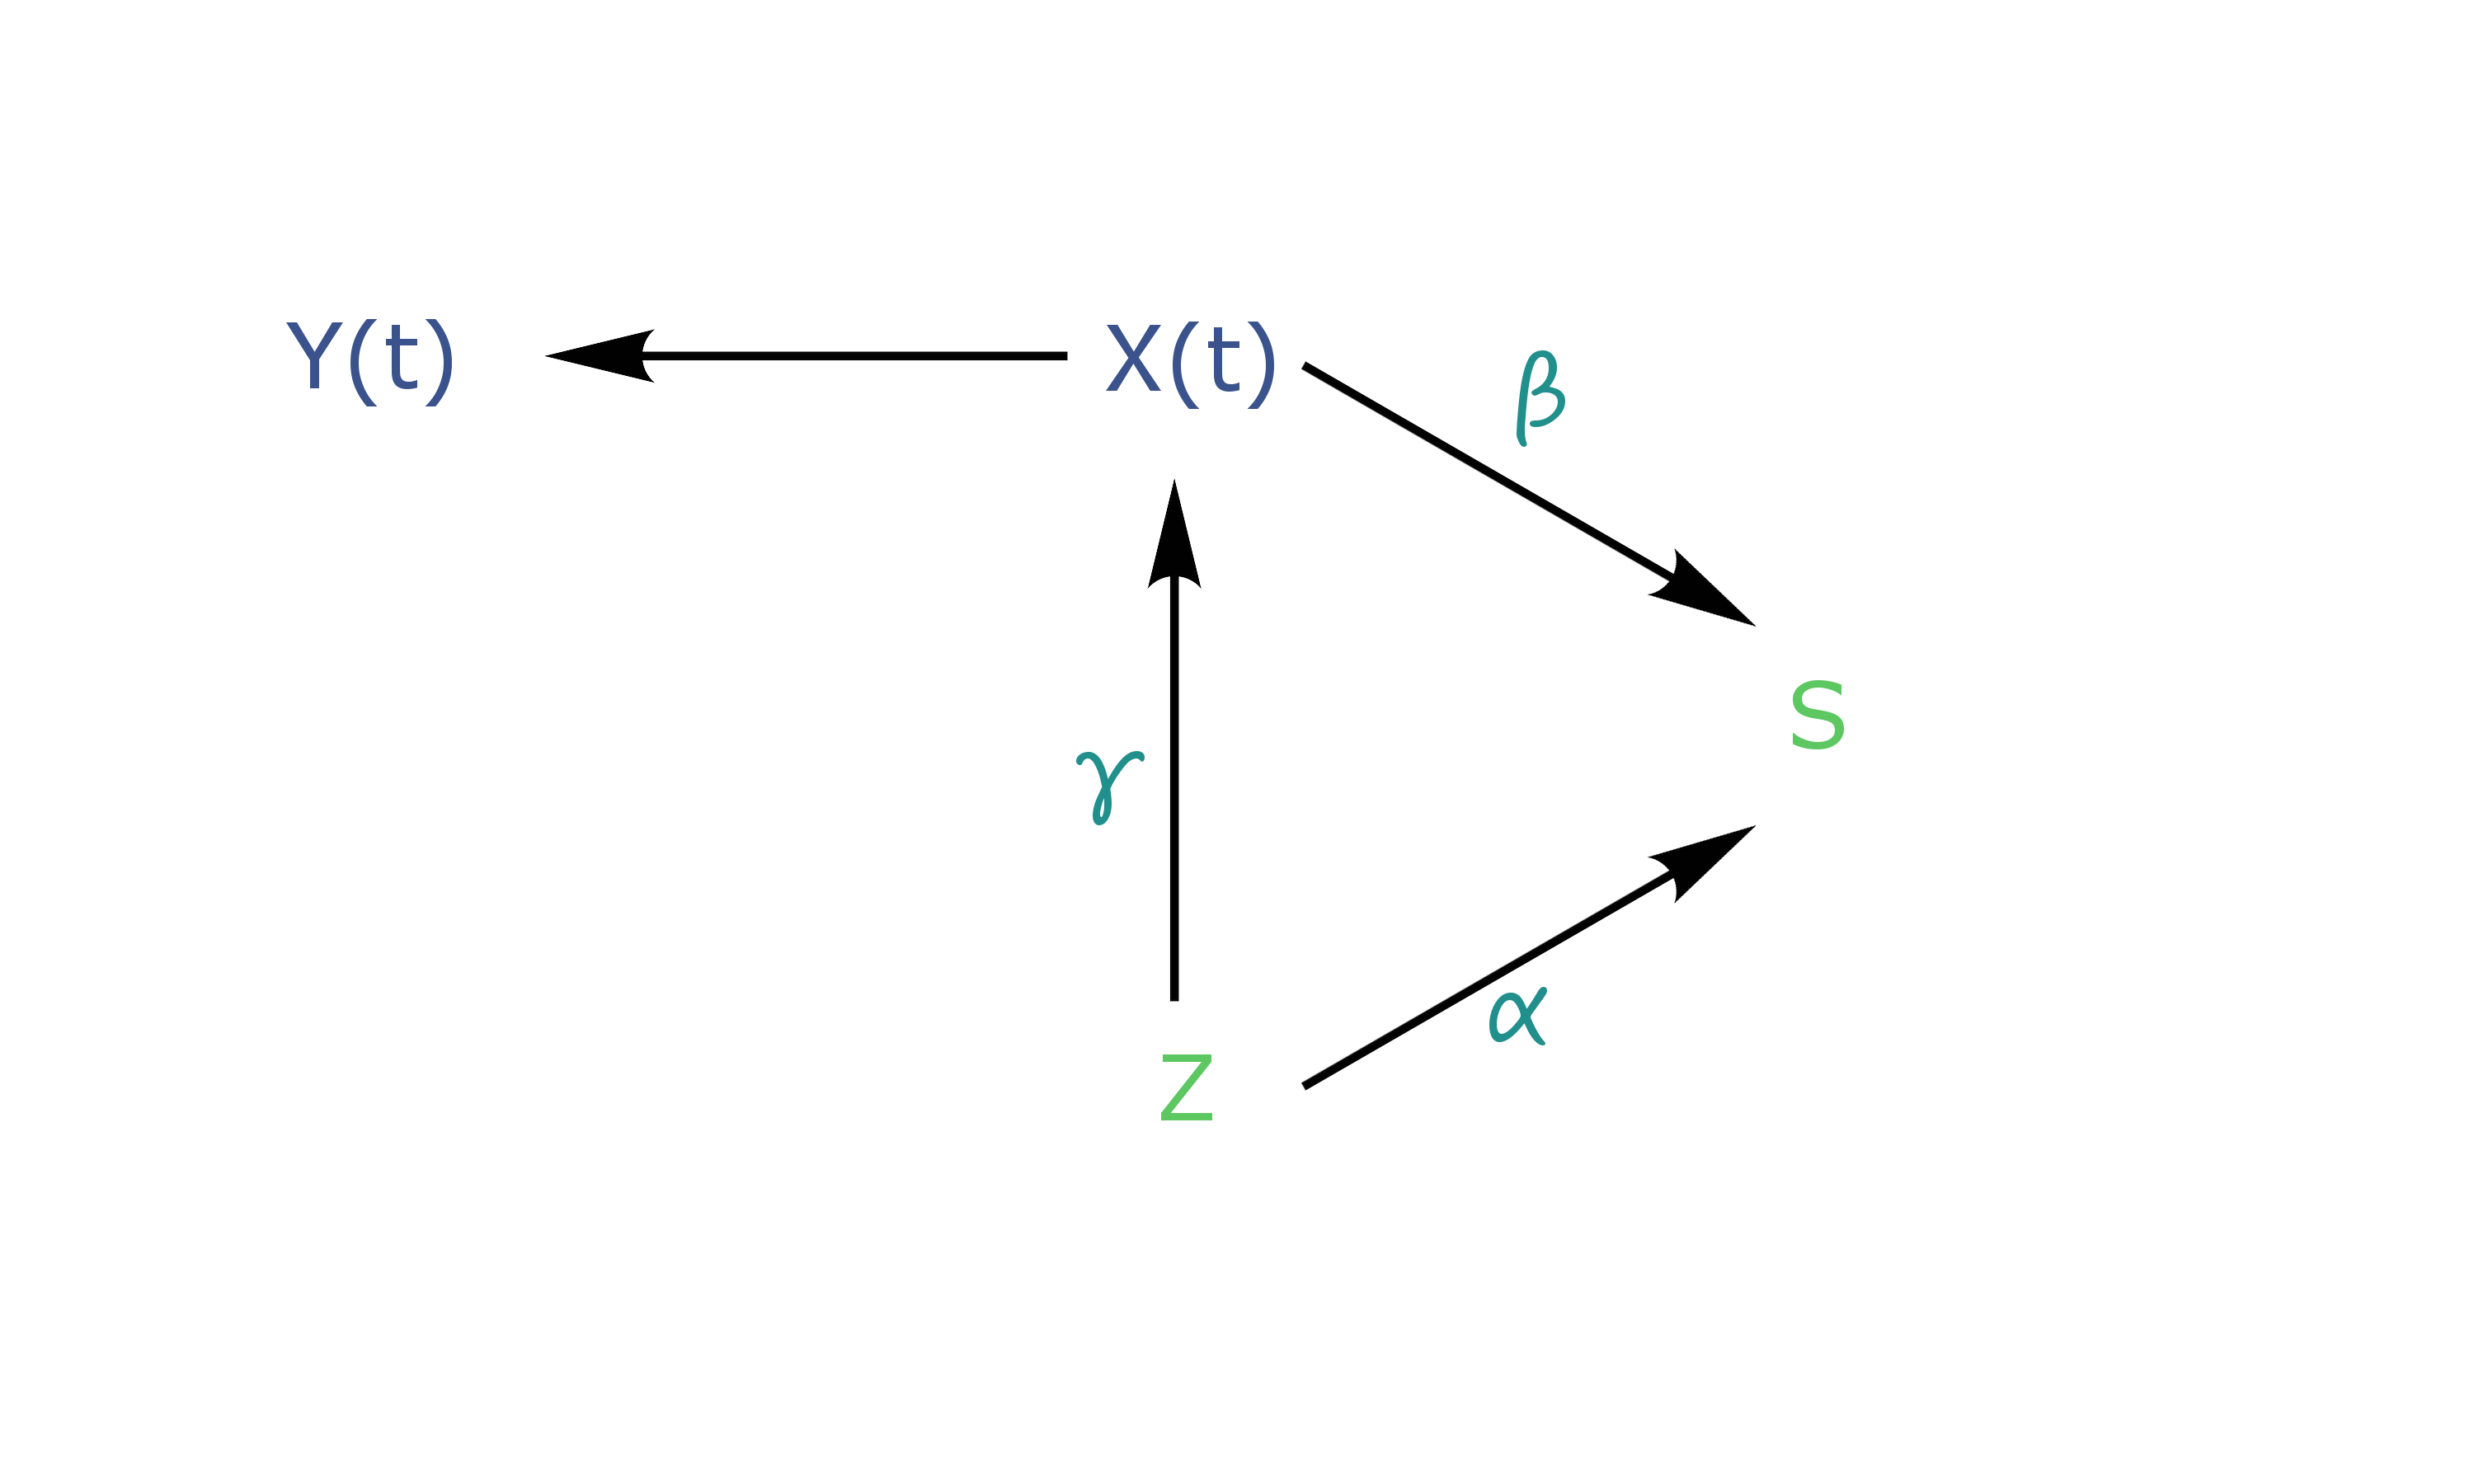
\includegraphics[width=5cm]{{images/jointmodel01.png}}}}
            \captionof{figure}{\color{springgreen3}Diagramme causal du Modèle Joint \mbox{(adapté de \citet{ibrahim_basic_2010})}.}
        \end{center}
        \vspace{1em}
    \end{minipage}%
    \hfill\vline\hfill
    \begin{minipage}[t]{0.475\columnwidth}%
	\vspace{1em}
        \begin{itemize}
            \setlength{\itemsep}{0.25em}
            \item[$X(t)$] trajectoire du biomarqueur générant les observations longitudinales $Y(t)$
            \item[$Y(t)$] données observées avec erreur de \mbox{mesure}
            \item[$S$] événement (survie) au temps $T$
            \item[$Z$] traitement (covariable)
            \item[$\alpha$] effet du traitement sur l’événement
            \item[$\beta$] effet de la trajectoire sur l’événement
            \item[$\gamma$] effet du traitement sur la trajectoire
         \end{itemize}
        \vspace{0.5em}
    \end{minipage}
\end{frame}


\begin{frame}{\subsecname: \subsubsecname}
    \vspace{-1em}
    \begin{minipage}[t]{0.475\columnwidth}
            \vspace{4em}
            \begin{center}
                {\color{black}\fbox{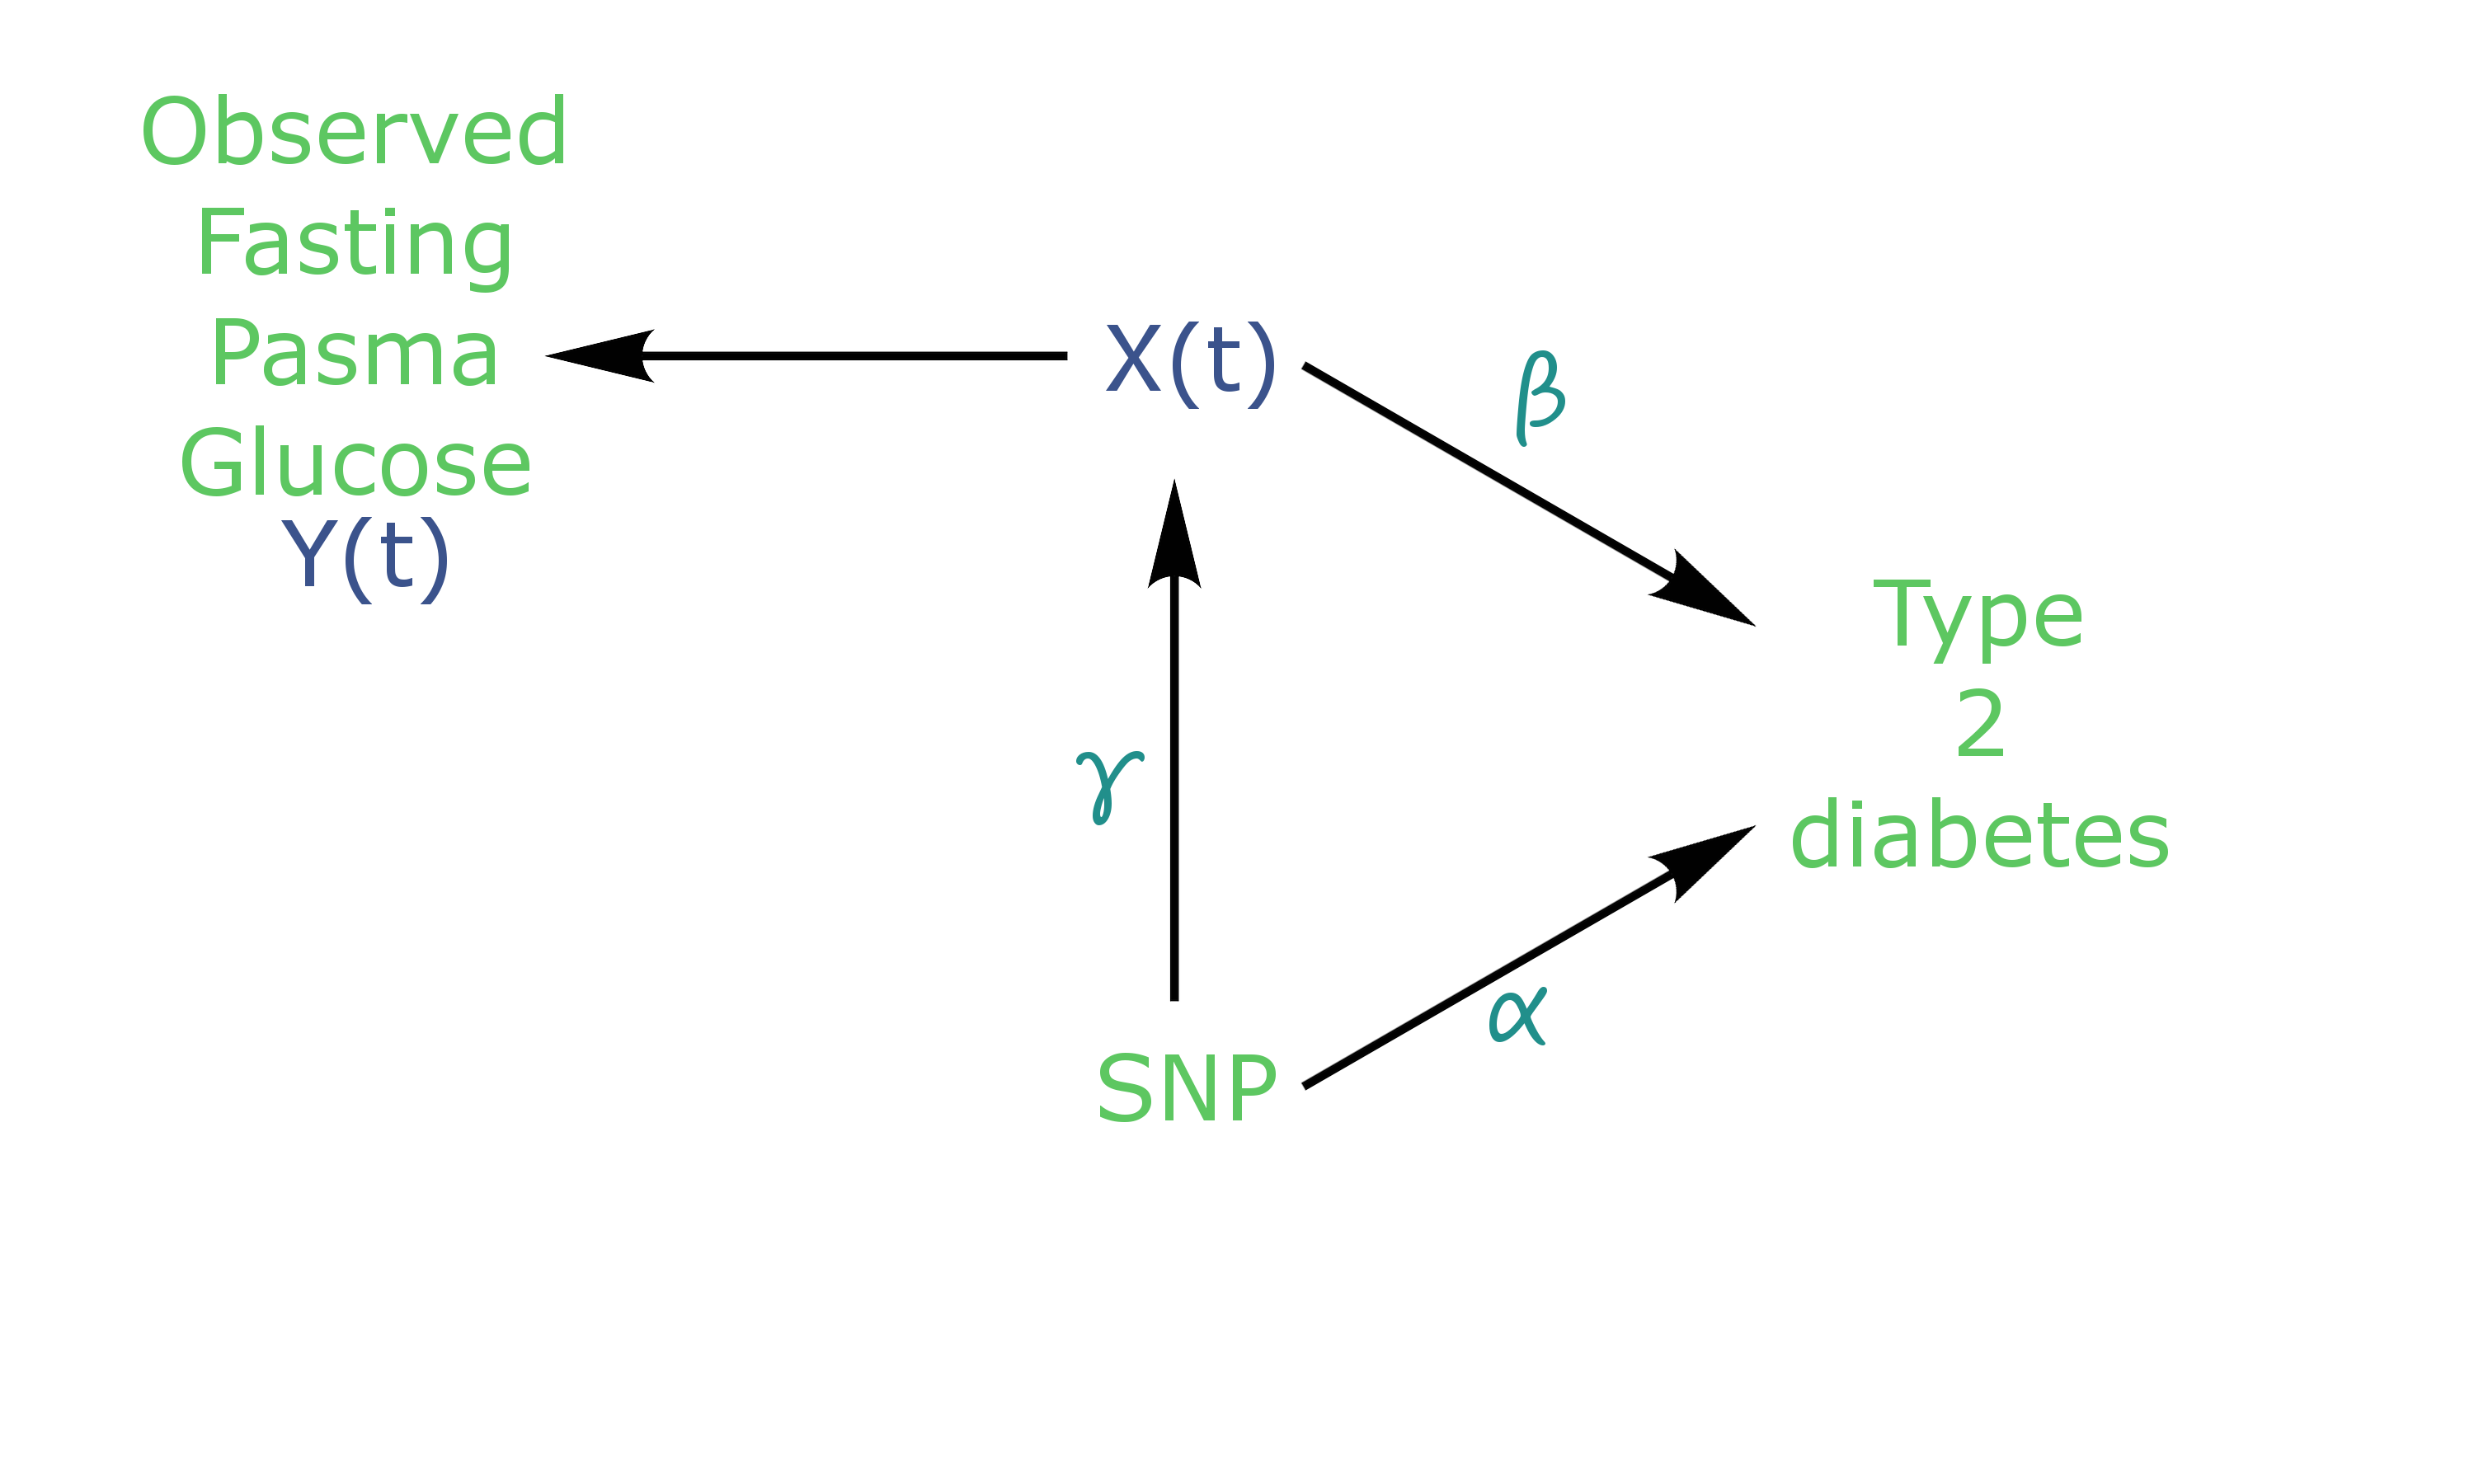
\includegraphics[width=5cm]{{images/jointmodel02.png}}}}
                \captionof{figure}{\color{springgreen3}Diagramme causal du Modèle Joint \mbox{(adapté de \citet{ibrahim_basic_2010})}.}
            \end{center}
        \vspace{1em}
    \end{minipage}%
    \hfill\vline\hfill
    \begin{minipage}[t]{0.475\columnwidth}%
	\vspace{1em}
        \begin{itemize}
            \setlength{\itemsep}{0.25em}
            \item[$X(t)$] trajectoire de \green{la glycémie} générant les observations longitudinales $Y(t)$
            \item[$Y(t)$] \green{glycémie} observée avec erreur de \mbox{mesure}
            \item[$S$] \green{survenue du diabète} au temps $T$
            \item[$Z$] \green{SNP} (Polymorphisme nucléotidique)
            \item[$\alpha$] effet du \green{SNP} sur \green{le diabète}
            \item[$\beta$] effet de \green{la glycémie} sur \green{le diabète}
            \item[$\gamma$] effet du \green{SNP} sur \green{la glycémie}
        \end{itemize}
        \vspace{0.5em}
    \end{minipage}
\end{frame}


\subsubsection{Motivation}
\begin{frame}{\subsecname: \subsubsecname}
	\par{Objectifs des études cliniques:}
	\begin{itemize}
		\item identifier un biomarqueur prognostique d'un événément clinique;
		\item effet d'un traitement sur un événement clinique \\(événement indépendant du traitement conditionnellement au biomarqueur).
	\end{itemize}
	\begin{center}\begin{minipage}[t]{0.85\textwidth}\vspace{-1.5em}\begin{exampleblock}{\itshape\textbf{Exemple}}\begin{description}
		\item[Biomarqueur] Glycémie à jeun
		\item[\'Evénement] Survenue d'un diabète de type 2
	\end{description}\end{exampleblock}\vspace{1.5em}\end{minipage}\end{center}
	\begin{center}\begin{minipage}[t]{0.85\textwidth}\vspace{-1.5em}\begin{block}{\itshape\textbf{Modèle de Cox à risque proportionnel étendu}}\setstretch{1}
		\vspace{-1em}\alt<2>{\begin{align}h(t)=h_0(t) \exp\{\beta Y(t) \textcolor{firebrick2}{+ \alpha Z}\}\end{align}}{\begin{align}h(t)=h_0(t) \exp(\beta Y(t)))\end{align}}
	\end{block}\vspace{1.5em}\end{minipage}\end{center}
\end{frame}


\subsubsection{Limitations}
\begin{frame}{\subsecname: \subsubsecname}
	\begin{itemize}
		\item Biomarqueur non mesurable en tout temps ou au temps de survenue de l’événement
			\begin{itemize}
				\item Mesure à des temps spécifiques ($t_{ij}$)
				\item Valeur manquante
				\item<2-8>[$\Rightarrow$] Imputation \visible<3-8>{\textcolor{firebrick2}{\textbf{$\textcolor{firebrick2}{\Rightarrow}$ Introduction de biais}}}
			\end{itemize}
		\item<4-8> Variabilité des mesures du biomarqueur
      		\item<5-8>[$\Rightarrow$] Mauvaise représentation de la ``vraie'' trajectoire ($Y_i(t_{ij}) \neq X_i(t_{ij})$)
      		\item<6-8> Nature ``endogène'' du biomarqueur
      		\item<7-8>[$\Rightarrow$] La trajectoire du biomarqueur est affectée par l'événement \visible<8>{\textcolor{firebrick2}{\textbf{$\textcolor{firebrick2}{\Rightarrow}$ Introduction de biais}}}
	\end{itemize}
\end{frame}


\subsubsection{Avantages}
\begin{frame}{\subsecname: \subsubsecname}
    \begin{itemize}
        \item Tester l'effet d'un SNP simultanément sur:
            \begin{itemize}
                \item le biomarqueur ($\gamma$);
                \item la survenue de l'événement ($\alpha$);
                \item le biomarqueur et la survenue de l'événement ($\beta\gamma+\alpha$).
            \end{itemize}
        \item<2> Gain de puissance statistique:
        \begin{itemize}
            \item<2> si $\beta\neq0$  (pour détecter un effet conjoint du SNP $\beta\gamma+\alpha\neq0$) \mbox{\citep{chen_sample_2011}};
            \item<2> par rapport à un modèle de ``Cox étendu'' (modèle de Cox avec covariable dépendante du temps).
        \end{itemize}
    \end{itemize}
\end{frame}


\subsection{Formulation}
\begin{frame}{\subsecname}
    \par{Dans le Modèle Joint, deux composantes (modèles) sont utilisées:}
	\begin{itemize}
		\item un modèle longitudinal est utilisé pour modéliser la ``vraie'' trajectoire du biomarqueur (non-observable),
		\item<2> et est incorporé en tant que covariable (latente) dépendante du temps dans un modèle de survie.
	\end{itemize}
\end{frame}


\subsubsection{Composante Longitudinale}
\begin{frame}{\subsecname: \subsubsecname}
    \begin{center}\begin{minipage}[t]{0.85\textwidth}\vspace{-1.5em}\begin{block}{\itshape\textbf{Composante longitudinale: modèle (linéaire) mixte}}\setstretch{1}
        Avec $T_i$, le temps d'événement et $C_i$, le temps de censure à droite: \begin{align}\tilde{T_i}&=\min(T_i, C_i),\end{align}
        avec $t_{ij}\leq \tilde{T_i}$, $j=1, \cdots, n_i$, où  $n_i$ est le nombre de mesures.\\[1.5em]
        Pour un individu $i$: \begin{align}Y_{i}(t_{ij})=X_{i}(t_{ij})+\epsilon_{i}(t_{ij})\end{align}
        Où: \begin{align}\epsilon_{i}(t_{ij}) \sim \mathcal{N}(0, \sigma^2)\end{align}
    \end{block}\vspace{1.5em}\end{minipage}\end{center}
\end{frame}


\begin{frame}{\subsecname: \subsubsecname}
    \vspace{-0.75em}
    \begin{center}\begin{minipage}[t]{0.85\textwidth}\vspace{-1.5em}\begin{block}{\itshape\textbf{Composante longitudinale: modèle (linéaire) mixte}}\setstretch{1}
        Pour un individu $i$: \begin{align}Y_{i}(t_{ij})=X_{i}(t_{ij})+\epsilon_{i}(t_{ij})\end{align}\\[1em]
        La trajectoire $X_i(t_{ij})$ peut être définie par un polynome, fonction du temps $t_{ij}$:
        \begin{align}
            X_{i}(t_{ij})=\theta_{0i} + \theta_{1i}t_{ij} + \cdots + \theta_{pi}t_{ij}^p &, & \boldsymbol\theta_p &\sim \mathcal{N}(\boldsymbol\mu_, \boldsymbol\Sigma)
        \end{align}
    \end{block}\vspace{1.5em}\end{minipage}\end{center}
    \vspace{-1em}
    \pause[2] \begin{center}\begin{minipage}[t]{0.85\textwidth}\vspace{-1.5em}\begin{exampleblock}{\itshape\textbf{Exemple: D.E.S.I.R.}}\setstretch{1}
        Avec $\textcolor{firebrick2}{W_i}$, la matrice des covariables d'ajustement (\^Age, Sexe et IMC)\newline
        et $\textcolor{firebrick2}{Z_i}$, le génotype du SNP d'intérêt:
        \begin{align}
            Y_{i}(t_{ij})=\theta_{0i} + \theta_{1i}t_{ij} \textcolor{firebrick2}{+ \gamma Z_i + \delta W_i} + \epsilon_{i}(t_{ij})\label{eq:LMM}
        \end{align}
    \end{exampleblock}\vspace{1.5em}\end{minipage}\end{center}
\end{frame}


\subsubsection{Composante de Survie}
\begin{frame}{\subsecname: \subsubsecname}
    \vspace{-0.5em}
    \begin{center}\begin{minipage}[t]{0.85\textwidth}\vspace{-1.5em}\begin{block}{\itshape\textbf{Composante de survie: modèle de Cox à risque proportionnel}}\setstretch{1}
        \alt<2->{
            Interrelation entre  $X_i(t)$, $T_i$ et $\textcolor{firebrick2}{W_i}$: \begin{align}
                h_i(t)&=\lim_{dt \to 0} \frac{P\{t\leq T_i<t+dt|T_i\geq t, \bar{Y_i}(t), \textcolor{firebrick2}{W_i}\}}{dt}\\
                &=h_0(t) \exp\{\beta X_{i}(t) \textcolor{firebrick2}{+ \eta W_i}\}
            \end{align}
        }{
            Interrelation entre  $X_i(t)$ et $T_i$: \begin{align}
                h_i(t)&=\lim_{dt \to 0} \frac{P\{t\leq T_i<t+dt|T_i\geq t, \bar{Y_i}(t)\}}{dt}\\
                &=h_0(t) \exp\{\beta X_{i}(t)\}
            \end{align}
        }
        Où $\bar{Y_i}(t)=\{Y_i(u),0 \leq u \leq t\}$ est l'historique de la trajectoire jusqu'au temps $t$.
    \end{block}\vspace{1.5em}\end{minipage}\end{center}
    \vspace{-1em}
    \pause[3] \begin{center}\begin{minipage}[t]{0.85\textwidth}\vspace{-1.5em}\begin{exampleblock}{\itshape\textbf{Exemple: D.E.S.I.R.}}\setstretch{1}
        Avec $\textcolor{firebrick2}{W_i}$, la matrice des covariables d'ajustement (\^Age, Sexe et IMC)\newline
        et $\textcolor{firebrick2}{Z_i}$, le génotype du SNP d'intérêt:
        \begin{align}
            h_i(t_{ij})&=h_0(t_{ij}) \exp\{\beta X_{i}(t_{ij}) \textcolor{firebrick2}{+ \alpha Z_i + \eta W_i}\}\label{eq:COX}
        \end{align}
    \end{exampleblock}\vspace{1.5em}\end{minipage}\end{center}
\end{frame}


\subsection{Test d'Hypothèse}
\begin{frame}{\subsecname}
Pour tester l'hypothèse nulle: \begin{gather*}\textcolor{black}{H_0:}\ \theta=\theta_0\ \textcolor{black}{(H_1:}\ \theta\neq\theta_0\textcolor{black}{)}\end{gather*}
\begin{description}
	\item[Test du Rapport de Vraisemblance] $LRT=-2\{\ell(\hat{\theta}_0)-\ell(\hat{\theta})\}$
	\item[Test de Wald] $W=(\hat{\theta}-\theta_0)^\top \mathcal{I}(\hat{\theta})(\hat{\theta}-\theta_0)$\quad (Univarié:$(\hat{\theta}_j-\theta_{0j})/\widehat{s.e.}(\hat{\theta}_j)$)
	\item[Test du Score] $U=S^\top(\hat{\theta}_0)\{\mathcal{I}(\hat{\theta}_0)\}^{-1}S(\hat{\theta}_0)$
\end{description}
\end{frame}

\subsection{\'Etude de Simulation}
\subsubsection{Objectifs}
\begin{frame}{\subsecname: \subsubsecname}
    \alt<2>{
        \begin{itemize}
            \item[$\Rightarrow$] Comparaison à une approche en ``deux-étapes'' (TS) \citep{tsiatis_modeling_1995}:
                \begin{center}\begin{minipage}[t]{0.85\textwidth}\vspace{-1.5em}\begin{block}{\itshape\textbf{``Two-Step''}}\setstretch{1.25}
\begin{itemize}
\item Première étape:
\vspace{-1.5em}\begin{gather*}
Y_{i}(t)=X_i(t)+ \epsilon_{i}(t)\\
X^*_{i}(t)=E\{X_{i}(t)|\bar{Y_i}(t), T_i\geq t\}
\end{gather*}\vspace{-1.5em}
\item Deuxième étape:
\vspace{-1.5em}\begin{gather*}
h_i(t)=h_0(t) \exp\{\beta X^*_{i}(t)\}
\end{gather*}
\end{itemize}
		\end{block}\vspace{1.5em}\end{minipage}\end{center}
        \end{itemize}
    }{
        \begin{itemize}
            \item Précision des estimateurs: RMSE (Root-Mean Square Error)
            	\begin{center}\begin{minipage}[t]{0.85\textwidth}\vspace{-1.5em}\begin{block}{\itshape\textbf{Root-Mean Square Error}}\setstretch{1}
               	 	\vspace{-1em}\begin{align}
                    		\operatorname{MSE}(\hat\theta)&= \operatorname{Biais}(\hat\theta)^2 + \operatorname{Var}(\hat\theta)\nonumber\\
                    		\operatorname{RMSE}(\hat{\theta})&=\sqrt{\operatorname{MSE}(\hat\theta)}\nonumber\\
                    		&=\sqrt{E\{(\hat{\theta}-\theta)^2\}}\nonumber
                	\end{align}
                \end{block}\vspace{1.5em}\end{minipage}\end{center}
            \item Faisabilité à l'échelle du génome: temps de calcul
        \end{itemize}
    }
\end{frame}


\subsubsection{Génération des Données}
\begin{frame}{\subsecname: \subsubsecname}
    Modèle longitudinale: $Y_{i}(t)=\theta_{0i} + \theta_{1i}t + \gamma Z_i + \epsilon_{i}(t)$\\
    Modèle de survie: $h_i(t)=h_0(t) \exp\{\beta X_{i}(t) + \alpha Z_i\}$
    \begin{center}\begin{minipage}[t]{0.85\textwidth}\vspace{-1.5em}\begin{block}{\itshape\textbf{Génération des temps d'événement: distribution exponentielle}}\setstretch{1}\vspace{-1em}\begin{gather*}
        \lambda>0\nonumber\\
        h_0(t)=\lambda\nonumber\\
        H_0(t)=\lambda t\nonumber\\
        H_i(T_i)=\int_0^{T_i}\lambda \exp(\beta X_i(t)+\alpha Z_i)dt\nonumber\\
        T_i=\frac{1}{\beta\theta_{1i}}\log\left(1-\frac{\beta\theta_{1i}\times \log(1-u)}{\lambda \exp(\beta\theta_{0i}+(\beta\gamma+\alpha)Z_i)}\right)\nonumber,\ u\sim\mathcal{U}(0,1)\nonumber\\
    \end{gather*}\end{block}\vspace{1.5em}\end{minipage}\end{center}
\end{frame}


\subsubsection{Paramètres de Simulation}
\begin{frame}{\subsecname: \subsubsecname}
    \begin{minipage}[c]{0.475\columnwidth}
        \begin{center}
            \captionof{figure}{\color{springgreen3}\citet{yaghootkar_recent_2013}}
               \alt<2>{{\color{black}\fbox{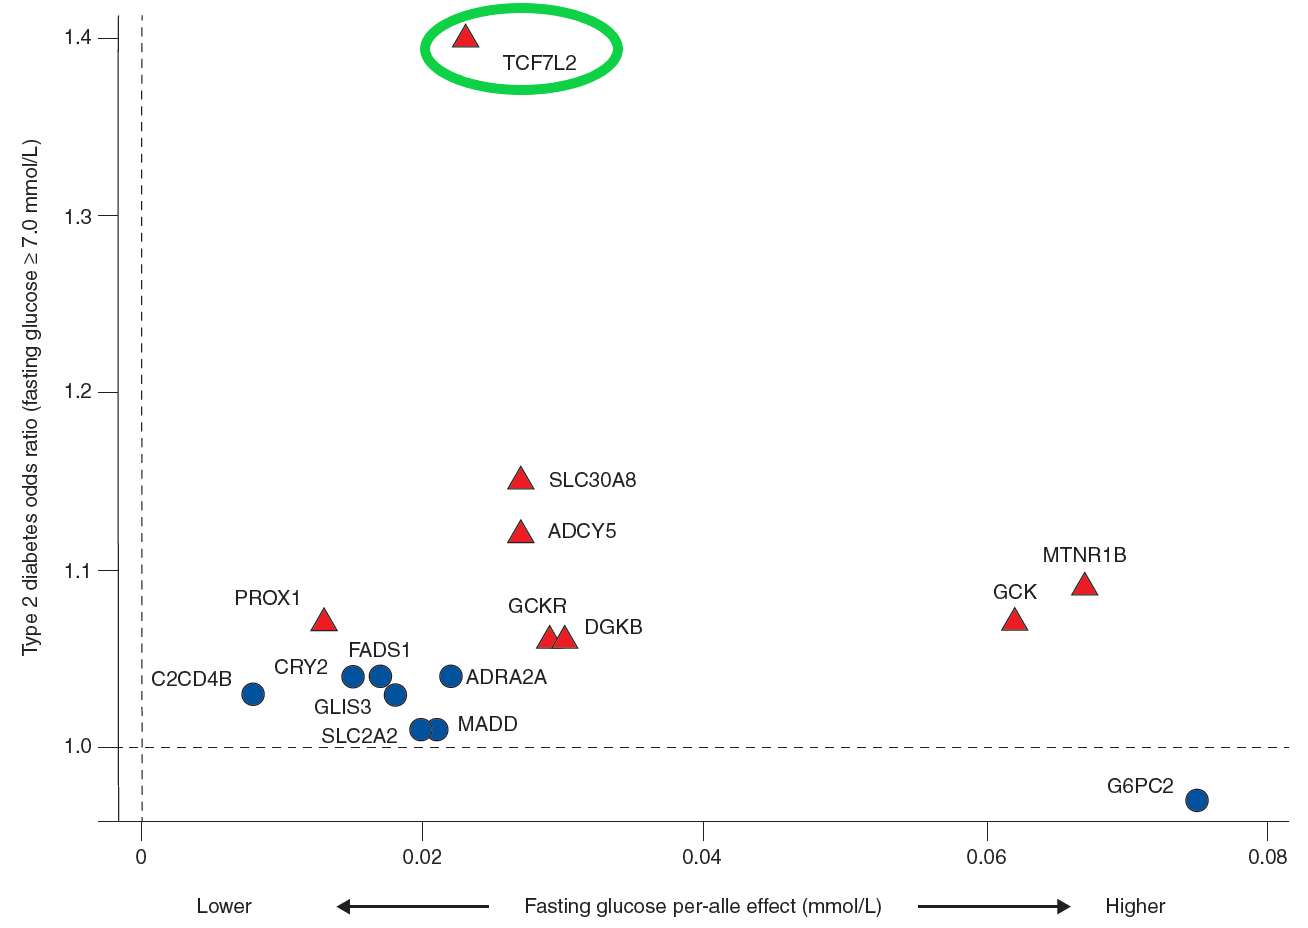
\includegraphics[width=5cm]{images/Yaghootkarb.png}}}}{{\color{black}\fbox{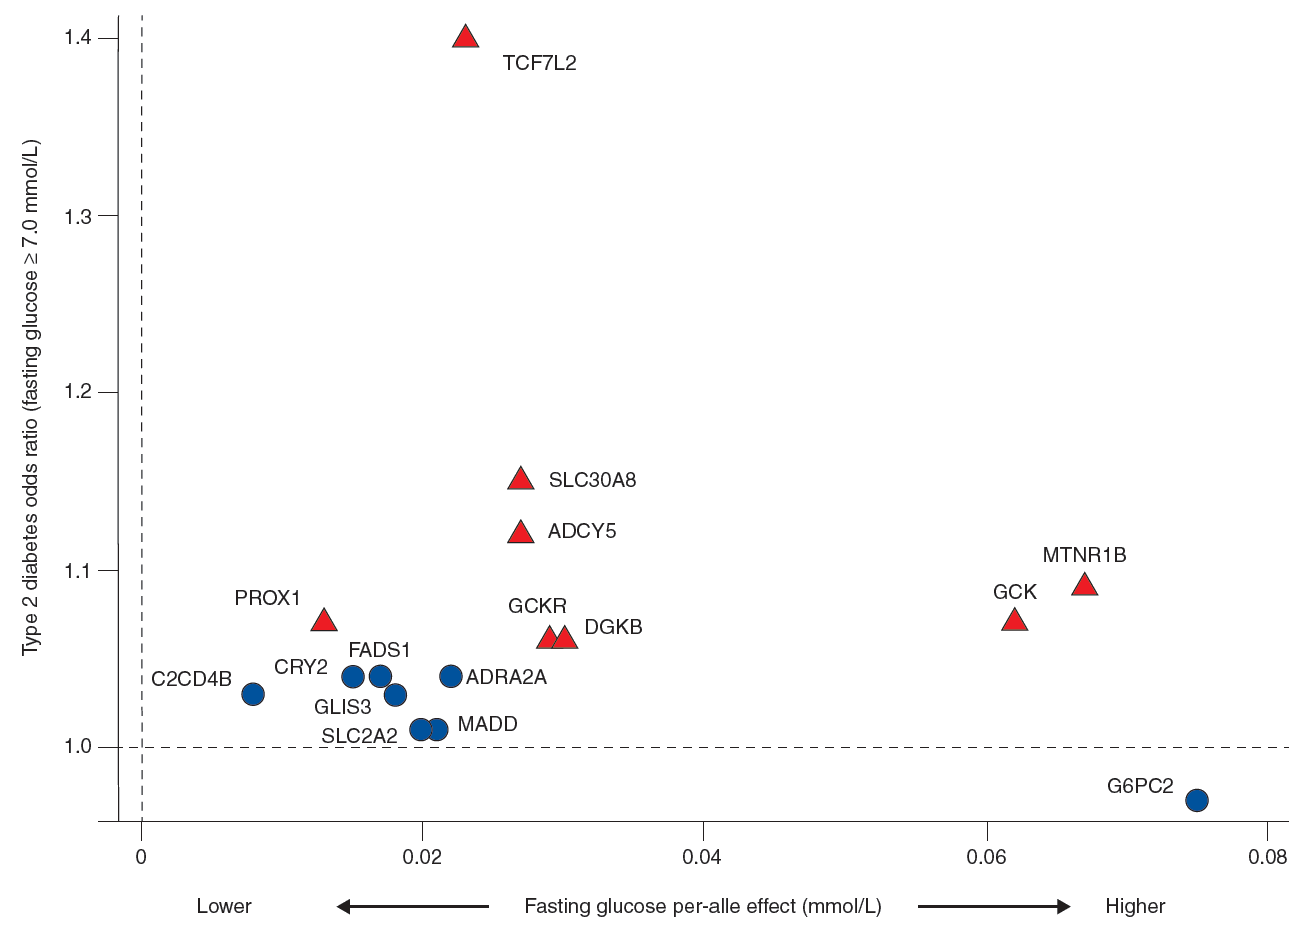
\includegraphics[width=5cm]{images/Yaghootkar.png}}}}
        \end{center}
    \end{minipage}%
    \hfill\vline\hfill
    \begin{minipage}[c]{0.475\columnwidth}%
        \begin{center}
            \captionof{figure}{\color{springgreen3}\citet{scott_large-scale_2012}}
               \alt<2>{{\color{black}\fbox{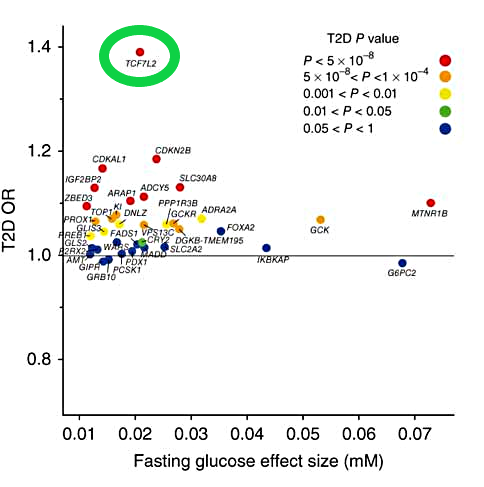
\includegraphics[width=5cm]{images/ng2385-F2b.png}}}}{{\color{black}\fbox{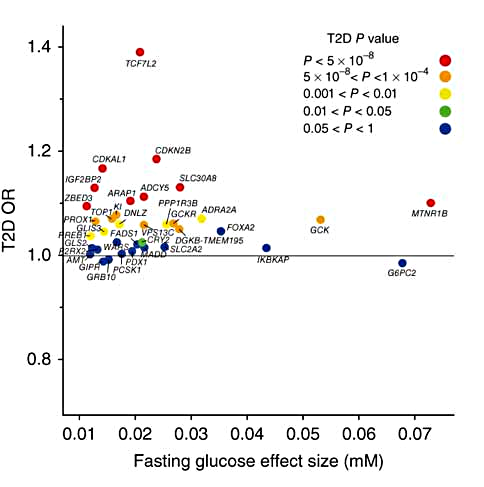
\includegraphics[width=5cm]{images/ng2385-F2.png}}}}
        \end{center}
    \end{minipage}
    \captionsetup{labelformat=empty, textfont={bf,it}, width=\textwidth}
    \captionof{figure}{\color{springgreen3}Taille d'effet $\textcolor{springgreen3}{\beta}$ et Odd Ratio respectivement pour la concentration de glucose et le diabète de type 2.}
\end{frame}


\begin{frame}{\subsecname: \subsubsecname}
    \everymath{\color{black}}
    \begin{center}
        \begin{table}
            {\small
                \begin{tabular}{lc}
                    \hline
                    Parameters & Values\\
                    \hline
                    Number of participants ($n$) & 4,352\\
                    Number of measures ($m$) & 4\\
                    Diabetes incidence rate ($d$) & 0.0384\\
                    Minor allele frequency ($f$) & 0.244\\
                    Random effects ($\theta$) & $\sim\mathcal{N}_2\left (\begin{bmatrix}4.55\\0.0108\end{bmatrix} , \begin{bmatrix} 0.143 & -0.00109 \\ -0.00109 & 6.8\times 10^{-04} \end{bmatrix} \right )$\\
                    SNP effect on $Y_{i}(t_{ij})$ ($\gamma$) & 0.0229\\
                    SNP effect on $T_i$ ($\alpha$) & 0.265\\
                    Association between $Y_{i}(t_{ij})$ and $T_i$ ($\beta$) & 3.17\\
                    Error term ($\epsilon$) & $\sim\mathcal{N}(0,0.305^2)$\\
                    \hline
                \end{tabular}
                \captionsetup{labelformat=empty, textfont={bf,it}, width=\textwidth}
                \captionof{table}{\color{springgreen3}Paramètres de simulation des données, basés sur rs17747324 (\textit{TCF7L2}).}
            }
        \end{table}
    \end{center}
    \everymath{\color{dodgerblue}}
\end{frame}


\begin{frame}{\subsecname: \subsubsecname}
    Puissance statistique pour détecter un effet joint du SNP rs17747324 (\textit{TCF7L2}), à partir de la formule développée par \citep{chen_sample_2011}:\\[1em]

    \begin{minipage}[t]{0.475\columnwidth}
        \vspace{0em}
        \begin{gather*}
            \textcolor{black}{H_0:\ }\beta\gamma+\alpha=0\\
            d=\frac{(z_{\tilde{\beta}}+z_{1-\tilde{\alpha}})^2}{f(1-f)(\beta\gamma+\alpha)^2}\\
            z_{\tilde{\beta}}=\pm\sqrt{df(1-f)(\beta\gamma+\alpha)^2}+z_{1-\tilde{\alpha}}
        \end{gather*}
    \end{minipage}%
    \hfill\vline\hfill
    \begin{minipage}[t]{0.475\columnwidth}%
        \vspace{1em}
        avec:
        \begin{description}
            \item[$d$] le nombre de T2D incidents,
            \item[$f$] la fréquence de l'allèle à risque,
            \item[$\tilde{\alpha}$] le seuil de significativité,
            \item[$\tilde{\beta}_{\tilde{\alpha}}$] la puissance statistique au seuil $\tilde{\alpha}$.
        \end{description}
        \vspace{1em}
    \end{minipage}
    \vspace{1em}
    \begin{center}$\textcolor{firebrick2}{\Rightarrow}\tilde{\beta}_{\tilde{\alpha}}=46,56\%$ pour rs17747324 (\textit{TCF7L2})\end{center}
\end{frame}


\subsubsection{Résultats}
\begin{frame}{\subsecname: \subsubsecname}
    \begin{center}
        {\color{black}\fbox{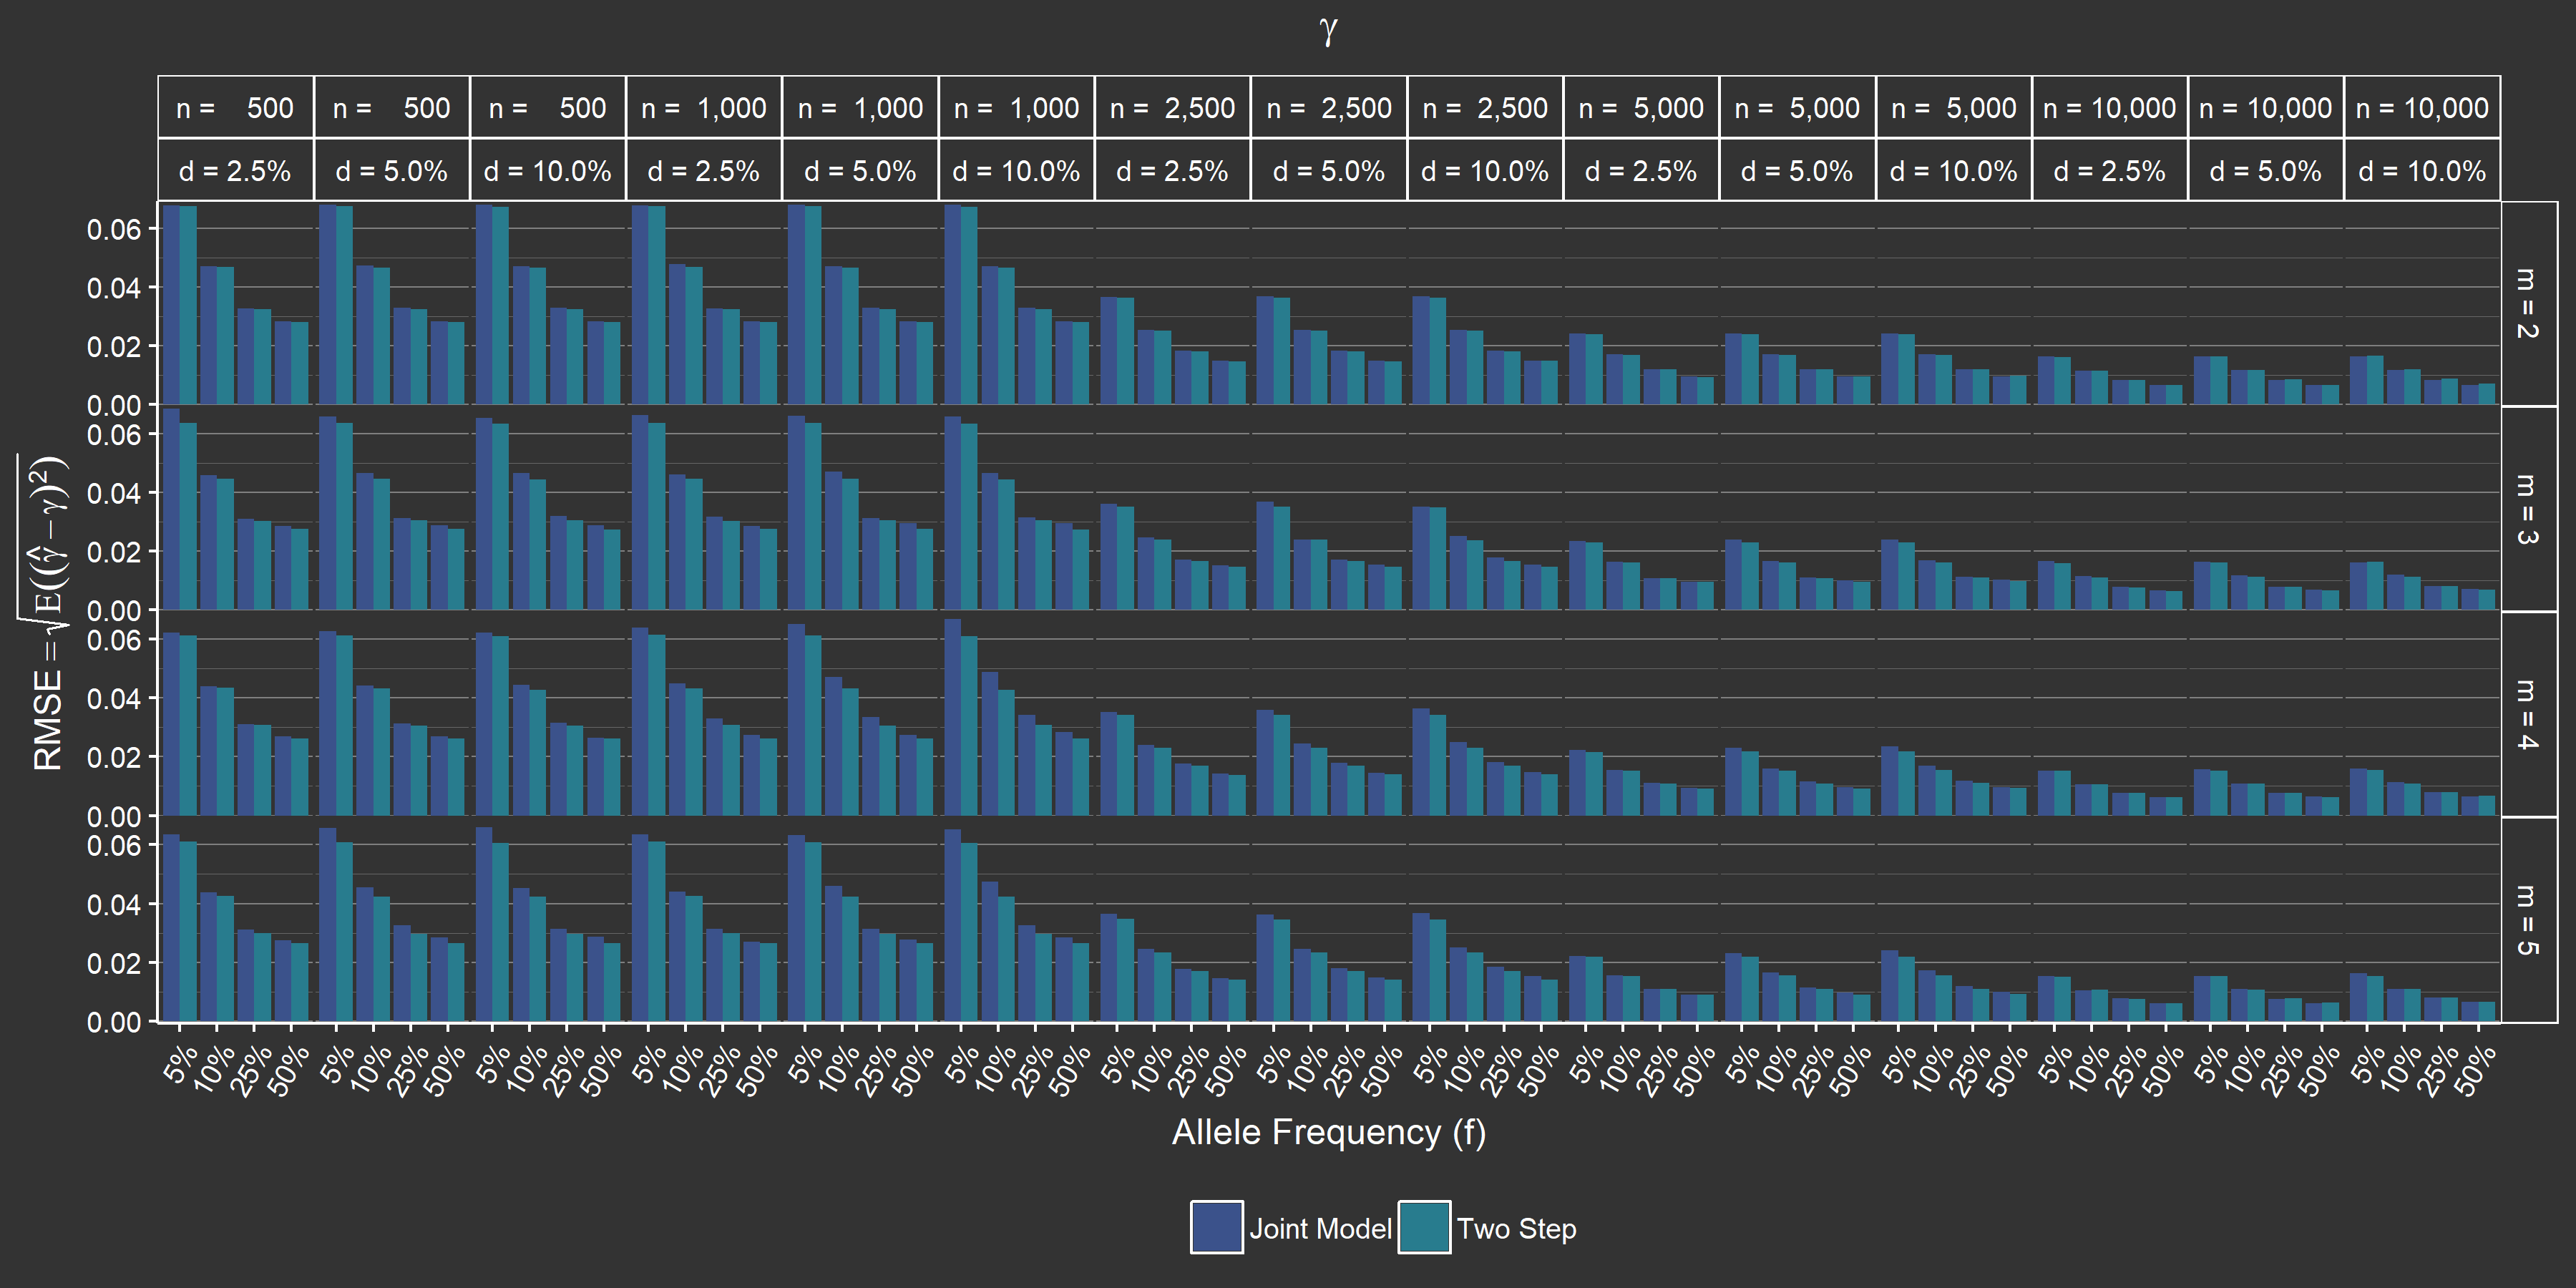
\includegraphics[width=0.95\textwidth]{{images/Fig10.png}}}}
        \captionsetup{labelformat=empty, textfont={bf,it}, width=0.95\textwidth}
        \captionof{figure}{\color{springgreen3}\'Etude de simulation de l'estmation $\color{springgreen3}\hat{\gamma}$ du Modèle Joint (extension \textit{JM}) et de l'approche en ``deux étapes'' (extension \textit{nlme}).}
    \end{center}
\end{frame}


\begin{frame}{\subsecname: \subsubsecname}
    \begin{center}
        {\color{black}\fbox{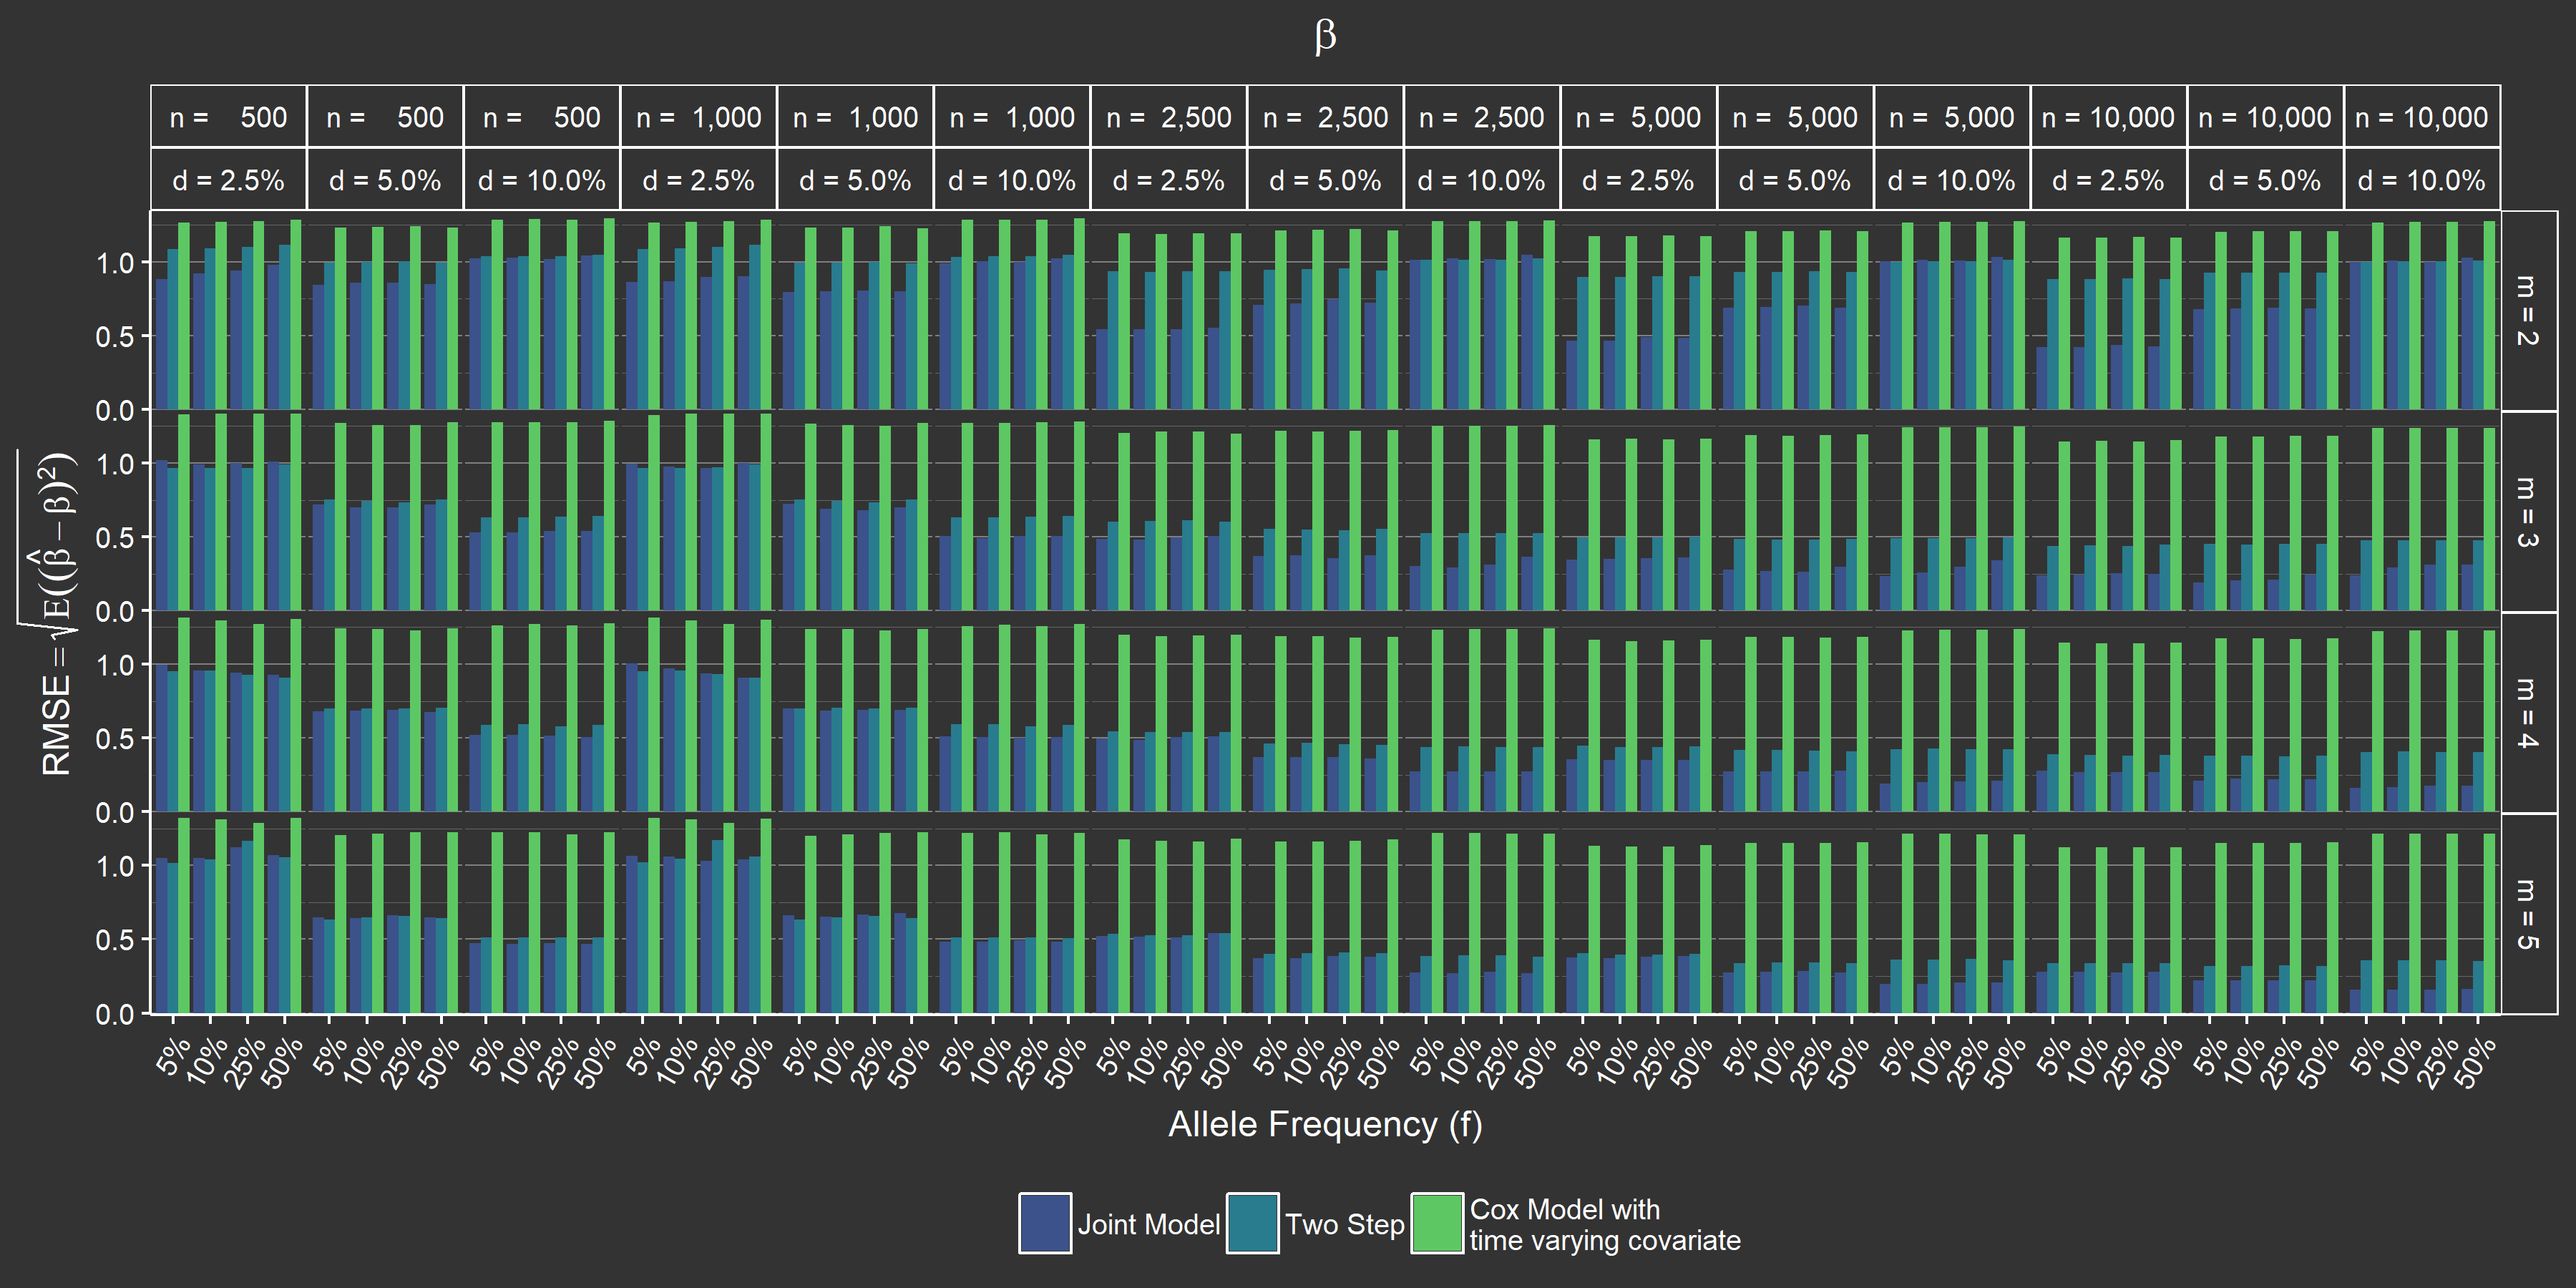
\includegraphics[width=0.95\textwidth]{{images/Fig11.png}}}}
        \captionsetup{labelformat=empty, textfont={bf,it}, width=0.95\textwidth}
        \captionof{figure}{\color{springgreen3}\'Etude de simulation de l'estmation $\color{springgreen3}\hat{\beta}$ du Modèle Joint (extension \textit{JM}) et de l'approche en ``deux étapes'' (extension \textit{nlme}).}
    \end{center}
\end{frame}


\begin{frame}{\subsecname: \subsubsecname}
    \begin{center}
        {\color{black}\fbox{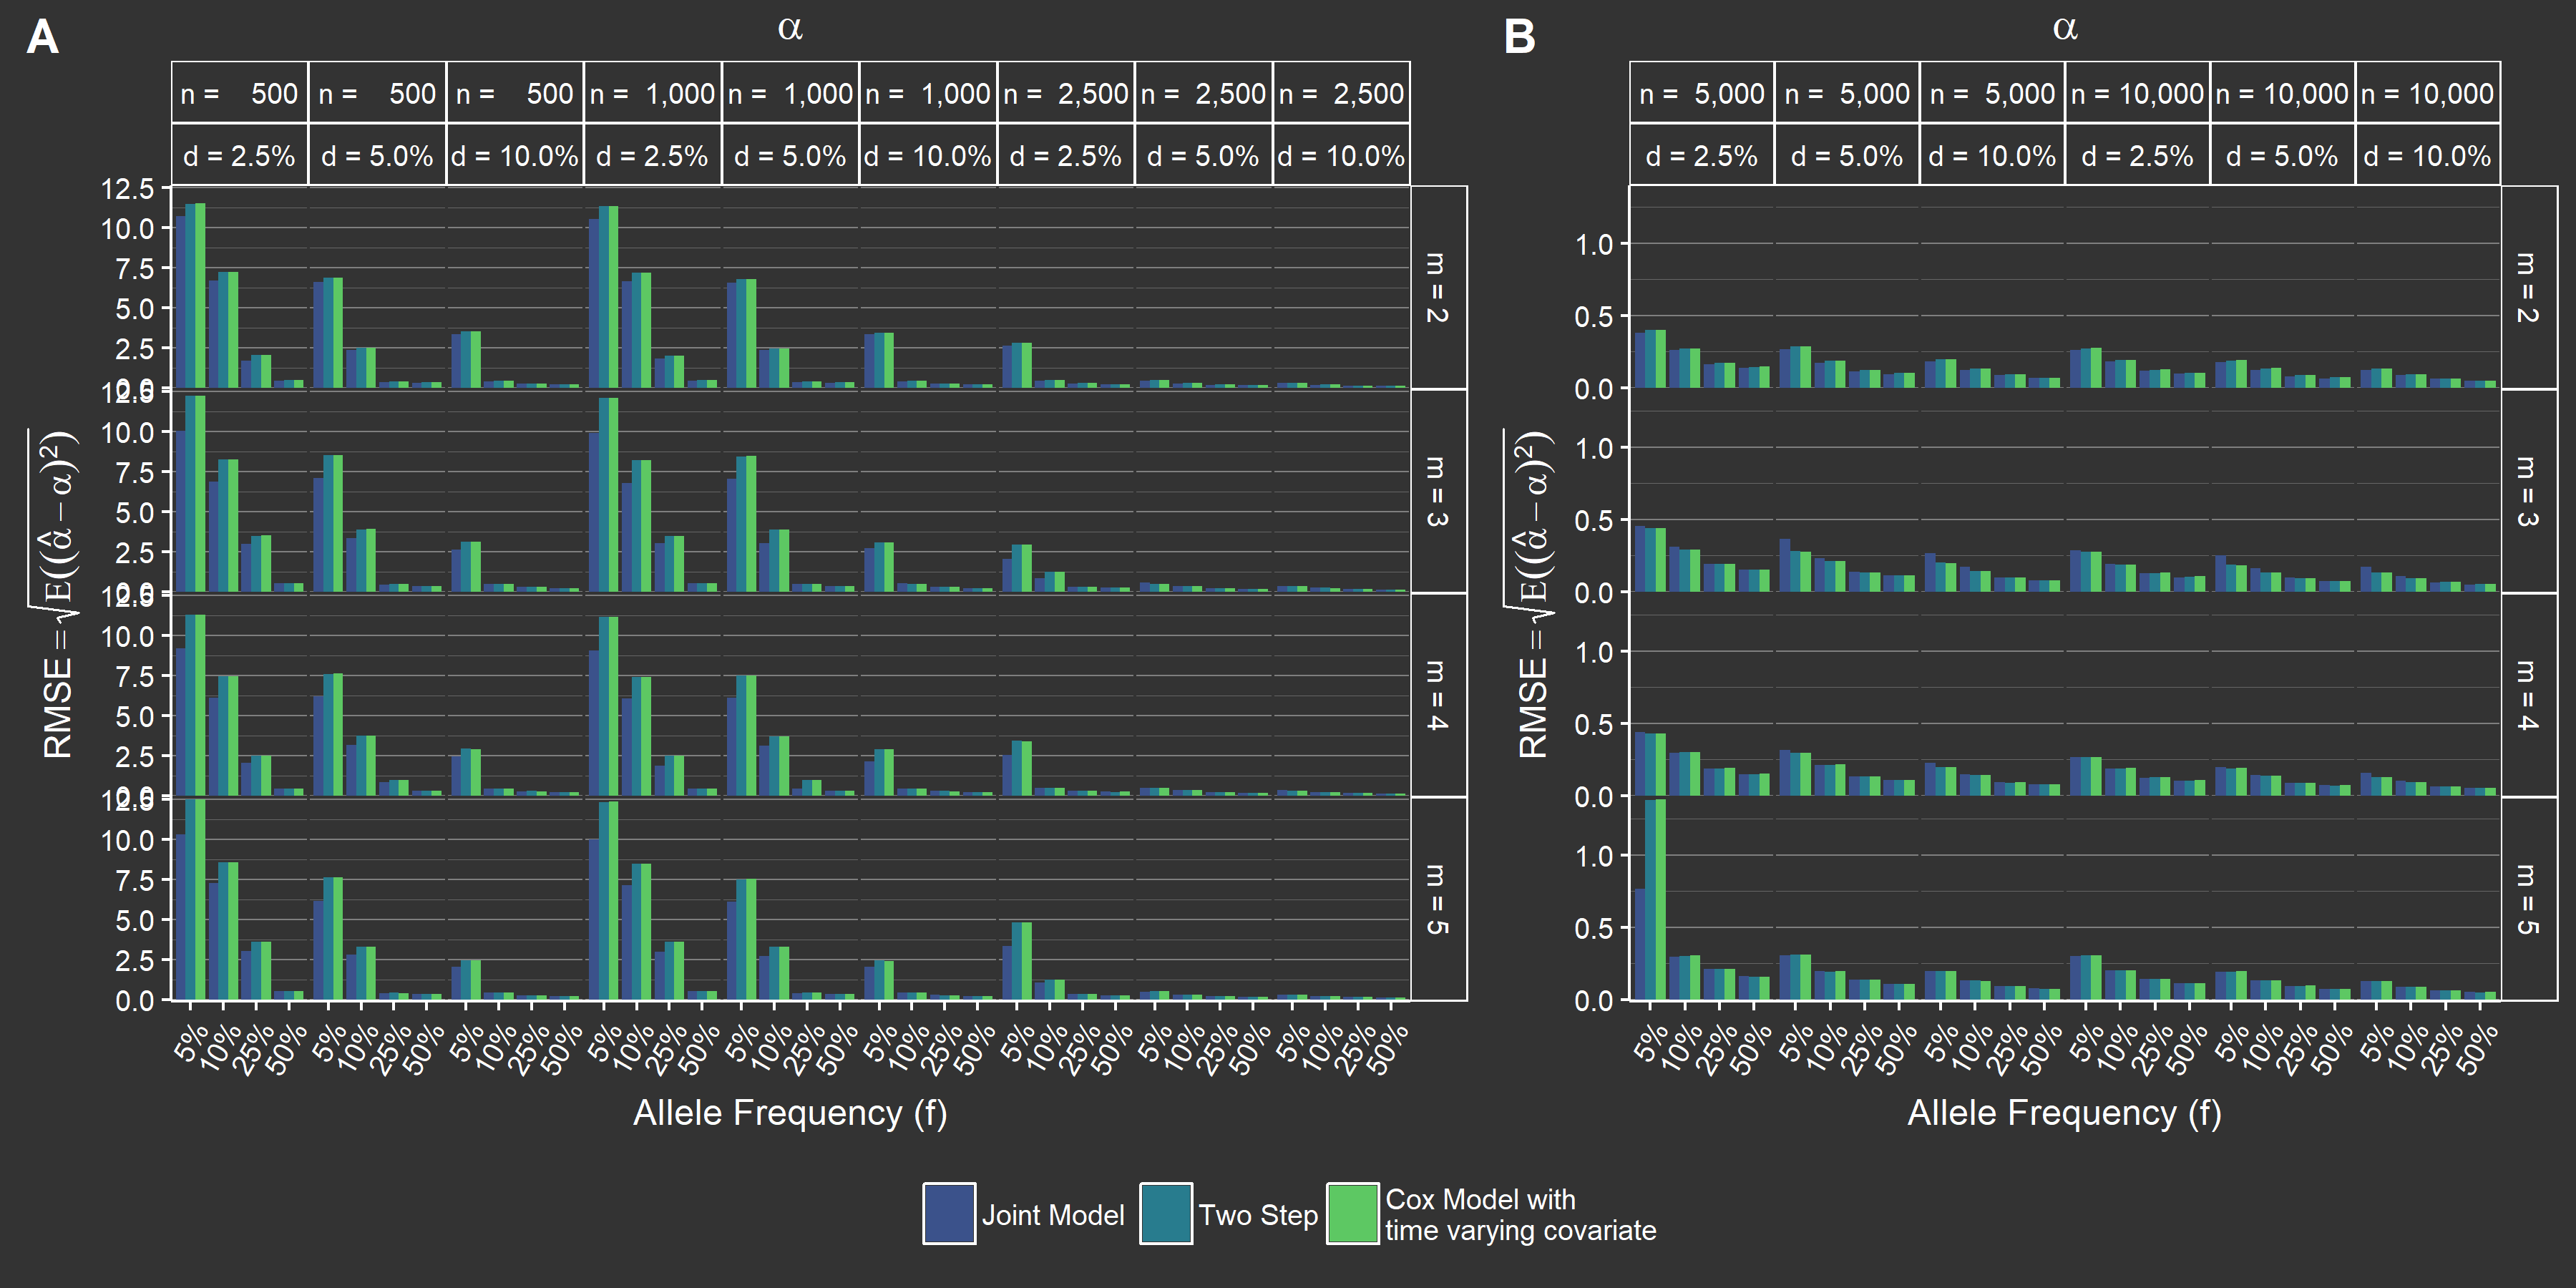
\includegraphics[width=0.95\textwidth]{{images/Fig09.png}}}}
        \captionsetup{labelformat=empty, textfont={bf,it}, width=0.95\textwidth}
        \captionof{figure}{\color{springgreen3}\'Etude de simulation de l'estmation $\color{springgreen3}\hat{\alpha}$ du Modèle Joint (extension \textit{JM}) et de l'approche en ``deux étapes'' (extension \textit{nlme}).}
    \end{center}
\end{frame}


\begin{frame}{\subsecname: \subsubsecname}
    \begin{center}
        {\color{black}\fbox{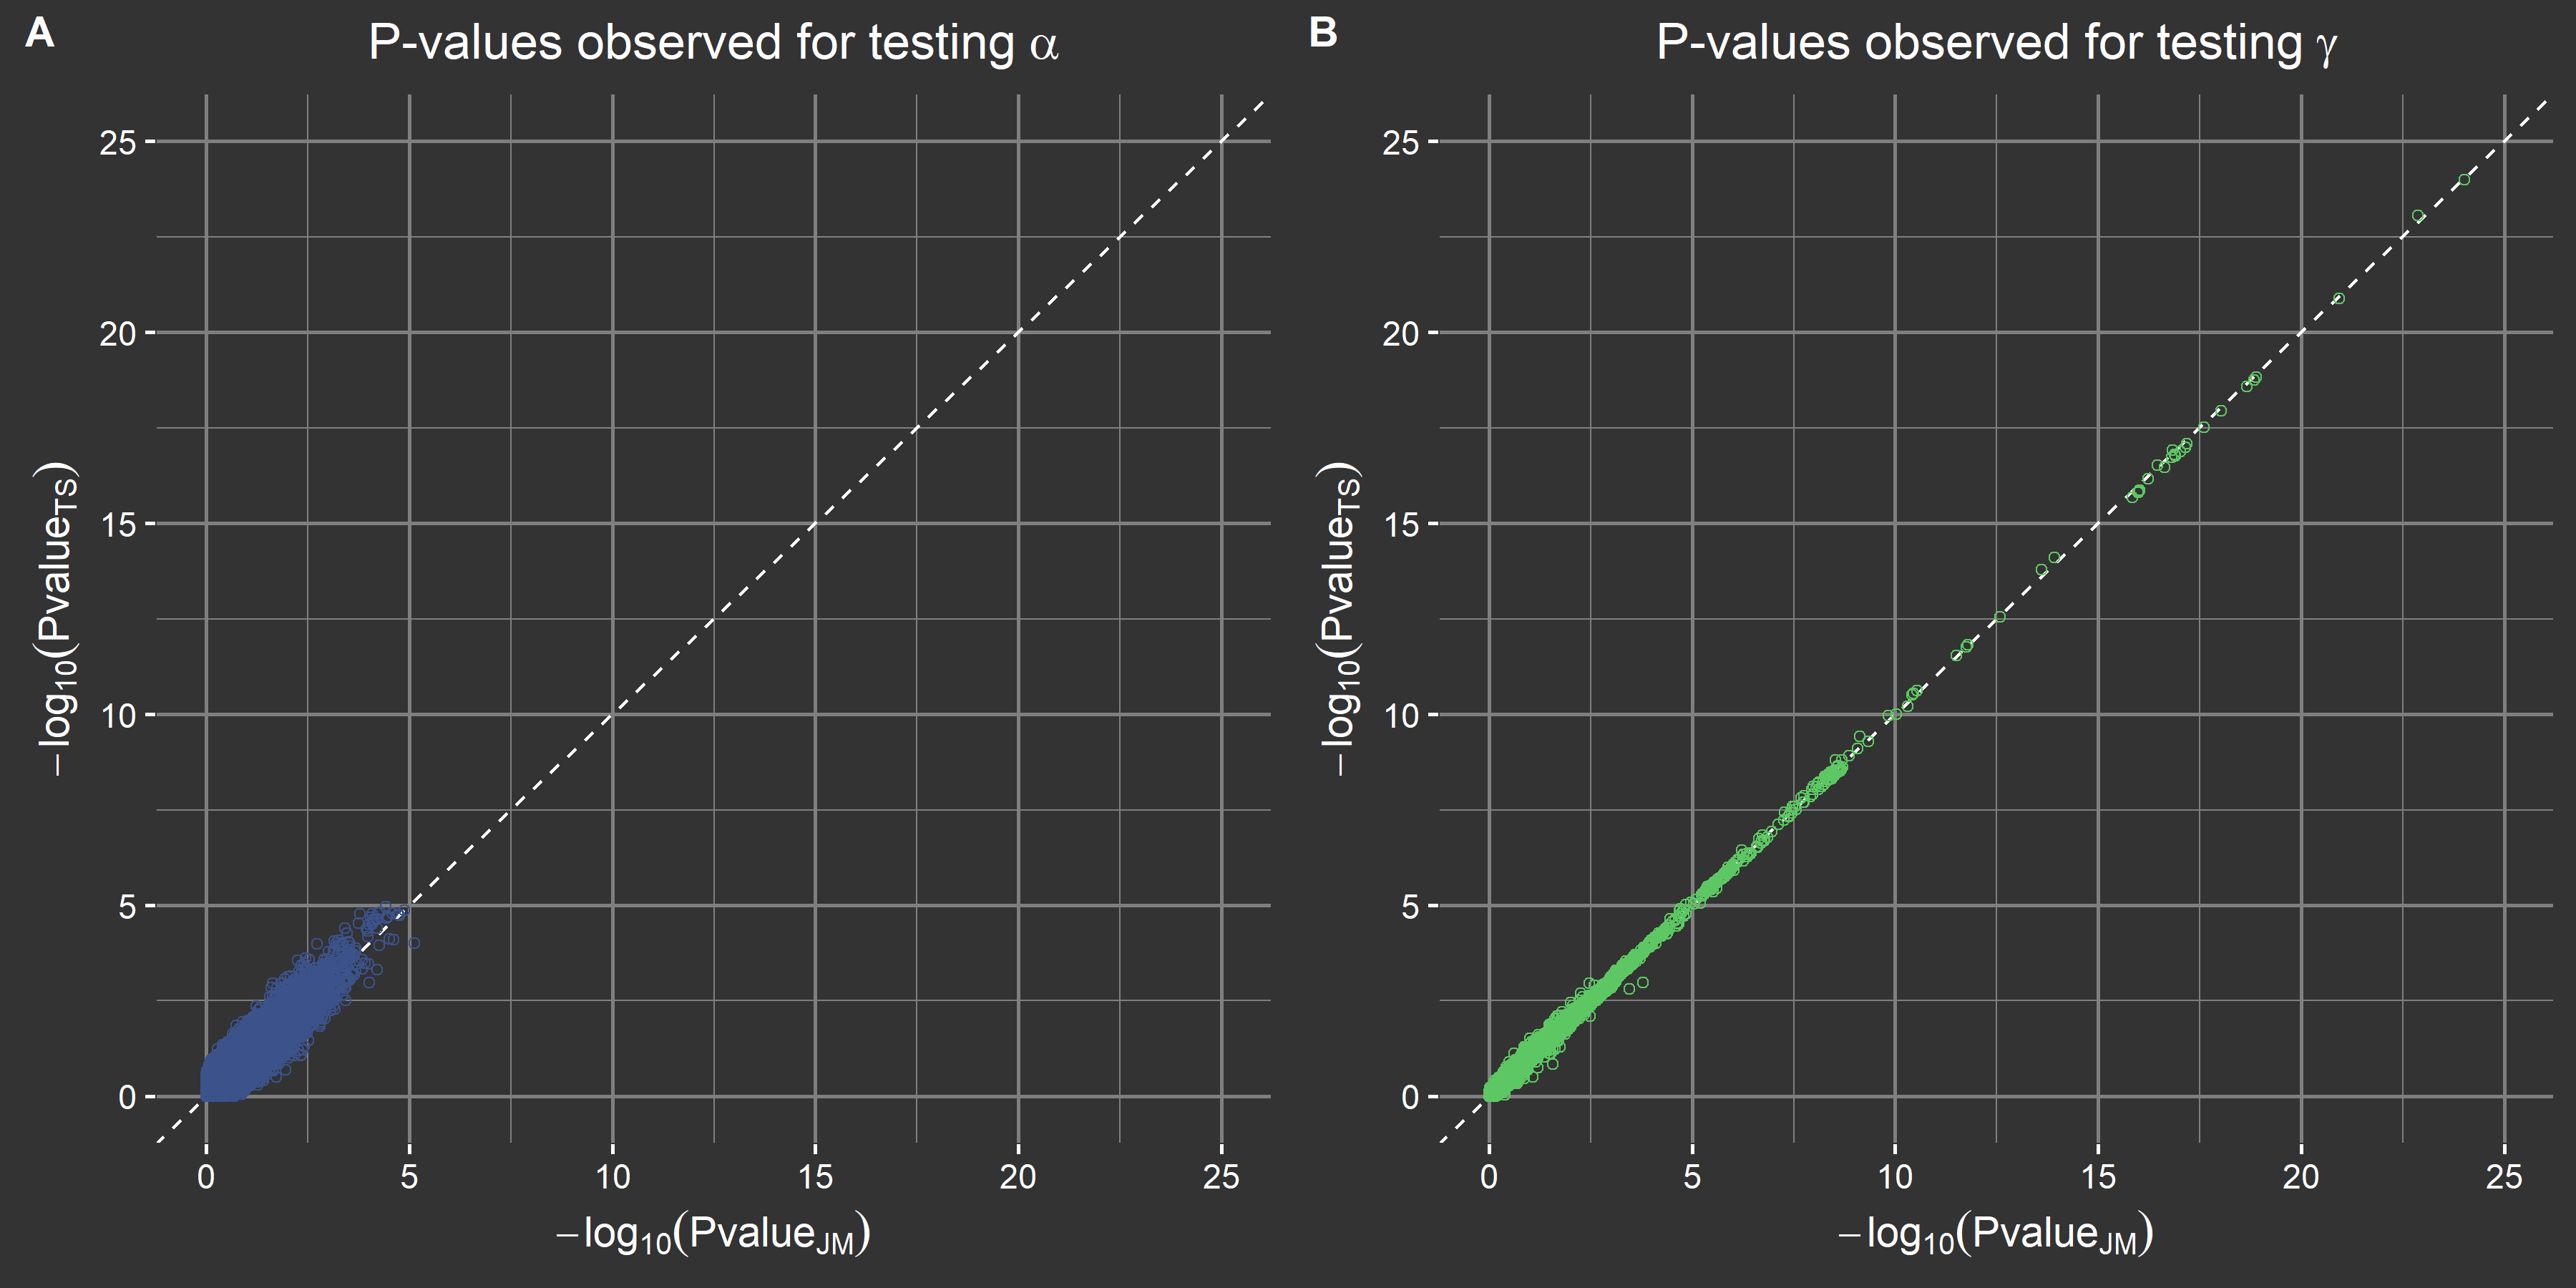
\includegraphics[width=0.95\textwidth]{{images/Fig15.png}}}}
        \captionsetup{labelformat=empty, textfont={bf,it}, width=0.95\textwidth}
        \captionof{figure}{\color{springgreen3}Comparaison des résultats des approches par Modèle Joint et en ``deux étapes''.}
    \end{center}
\end{frame}


\begin{frame}{\subsecname: \subsubsecname}
    \begin{center}
        {\color{black}\fbox{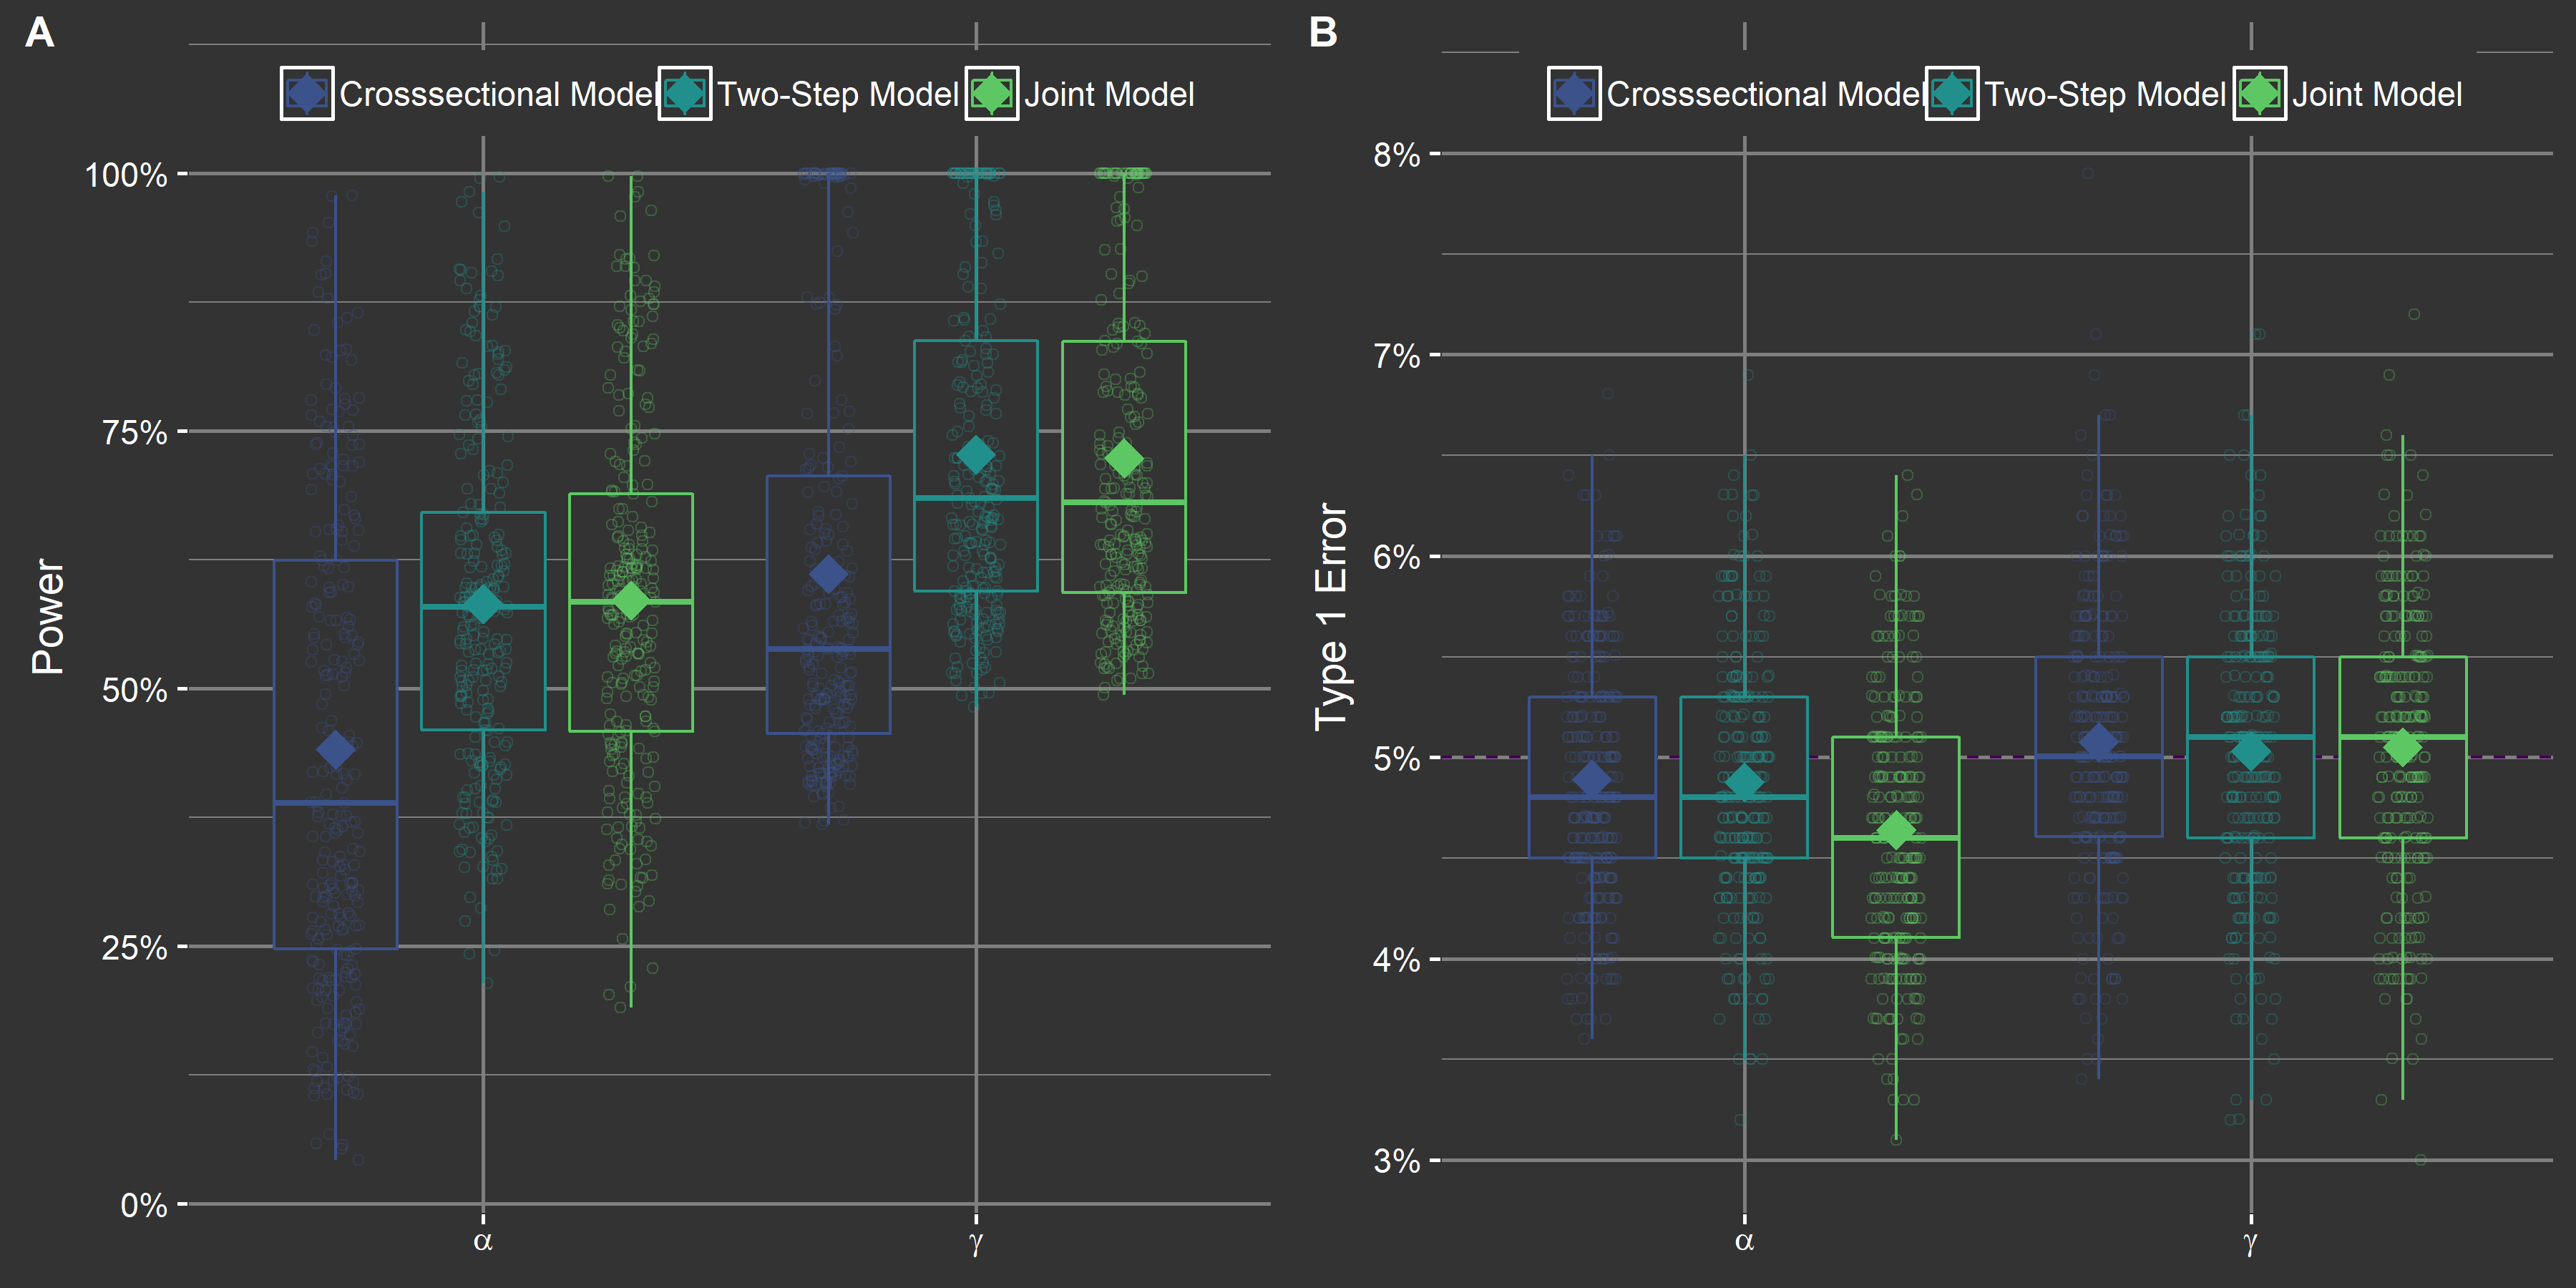
\includegraphics[width=0.95\textwidth]{{images/Fig12.png}}}}
        \captionsetup{labelformat=empty, textfont={bf,it}, width=0.95\textwidth}
        \captionof{figure}{\color{springgreen3}Comparaison des résultats des approches par Modèle Joint et en ``deux étapes''.}
    \end{center}
\end{frame}


\begin{frame}{\subsecname: \subsubsecname}
    \everymath{\color{black}}
    \begin{center}
        \begin{table}
            \begin{tabular}{ccccc}
                \hline
                & \multicolumn{2}{c}{\textcolor<2>{maroon2}{Modèle Joint}} & \multicolumn{2}{c}{\textcolor<2>{dodgerblue}{Modèle ``deux-étapes''}}\\
                \hline
                Nombre & \textcolor<2>{maroon2}{Moyenne} & \multirow{2}{*}{\textcolor<2>{maroon2}{100K SNPs}} & \textcolor<2>{dodgerblue}{Moyenne} & \multirow{2}{*}{\textcolor<2>{dodgerblue}{100K SNPs}}\\
                d'individu & \textcolor<2>{maroon2}{(\'Ecart-Type)} &  & \textcolor<2>{dodgerblue}{(\'Ecart-Type)} & \\
                \hline
                500 & \textcolor<2>{maroon2}{51 s ($\textcolor<2>{maroon2}{3,4}$)} & \textcolor<2>{maroon2}{59 j} & \textcolor<2>{dodgerblue}{$\textcolor<2>{dodgerblue}{0,71}$ s ($\textcolor<2>{dodgerblue}{0,066}$)} & \textcolor<2>{dodgerblue}{$\textcolor<2>{dodgerblue}{0,82}$ j}\\
                2\ 500 & \textcolor<2>{maroon2}{100 s (11)} & \textcolor<2>{maroon2}{120 j} & \textcolor<2>{dodgerblue}{$\textcolor<2>{dodgerblue}{3,1}$ s ($\textcolor<2>{dodgerblue}{0,092}$)} & \textcolor<2>{dodgerblue}{$\textcolor<2>{dodgerblue}{3,6}$ j}\\
                5\ 000 & \textcolor<2>{maroon2}{180 s (25)} & \textcolor<2>{maroon2}{210 j} & \textcolor<2>{dodgerblue}{$\textcolor<2>{dodgerblue}{6,3}$ s ($\textcolor<2>{dodgerblue}{0,17}$)} & \textcolor<2>{dodgerblue}{$\textcolor<2>{dodgerblue}{7,3}$ j}\\
                10\ 000 & \textcolor<2>{maroon2}{340 s (34)} & \textcolor<2>{maroon2}{400 j} & \textcolor<2>{dodgerblue}{9 s ($\textcolor<2>{dodgerblue}{0,22}$)} & \textcolor<2>{dodgerblue}{10 j}\\
                \hline
            \end{tabular}
            \captionof{table}{\color{springgreen3}Temps de calcul (fonction \textit{system.time} du logiciel R).}
        \end{table}
    \end{center}
    \everymath{\color{dodgerblue}}
\end{frame}


\subsection{Application sur Données Réelles: D.E.S.I.R.}
\begin{frame}{\subsecname}
    \vspace{-1em}
    \begin{center}\begin{minipage}[t]{0.85\textwidth}\vspace{-1.5em}\begin{block}{\itshape\textbf{D.E.S.I.R.}}\setstretch{1}
        \begin{itemize}
            \item Données Épidémiologiques sur le Syndrome d’Insulino-Résistance
            \item 5\ 212 individus
            \item 1 visite tous les 3 ans, de 0 à 9 ans
            \item \texttildelow 4\ 500 individus génotypés
        \end{itemize}
    \end{block}\vspace{1.5em}\end{minipage}\end{center}
    \vspace{-1em}
    \begin{minipage}[t]{0.475\columnwidth}
        \vspace{-3.75em}
        \everymath{\color{black}}
        \begin{center}
            \begin{table}
                {\footnotesize
                    \begin{tabular}{lcc}
                        \hline
                         &  Témoins &  Cas Incidents \\
                        \hline
                        Sexe & \Male$2\ 293$; \Female$2\ 483$ & \Male$142$; \Female$64$ \\
                        \^Age (années) & $46$ ($10$) & $51$ ($9$) \\
                        Glycémie (mmol/L) & $5,2$ ($0,51$) & $6$ ($0,57$)\\
                        BMI & $24$ ($3,7$) & $28$ ($4,4$) \\
                        HbA1c (\%) & $5,4$ ($0,39$) & $5,8$ ($0,48$) \\
                        \hline
                    \end{tabular}
                }
                \captionof{table}{\color{springgreen3}Caractéristiques des individus D.E.S.I.R. selon le statut diabète de type 2.}
            \end{table}
        \end{center}
        \everymath{\color{dodgerblue}}
    \end{minipage}%
    \hfill\vline\hfill
    \begin{minipage}[c]{0.475\columnwidth}%
        \begin{center}
            {\color{black}\fbox{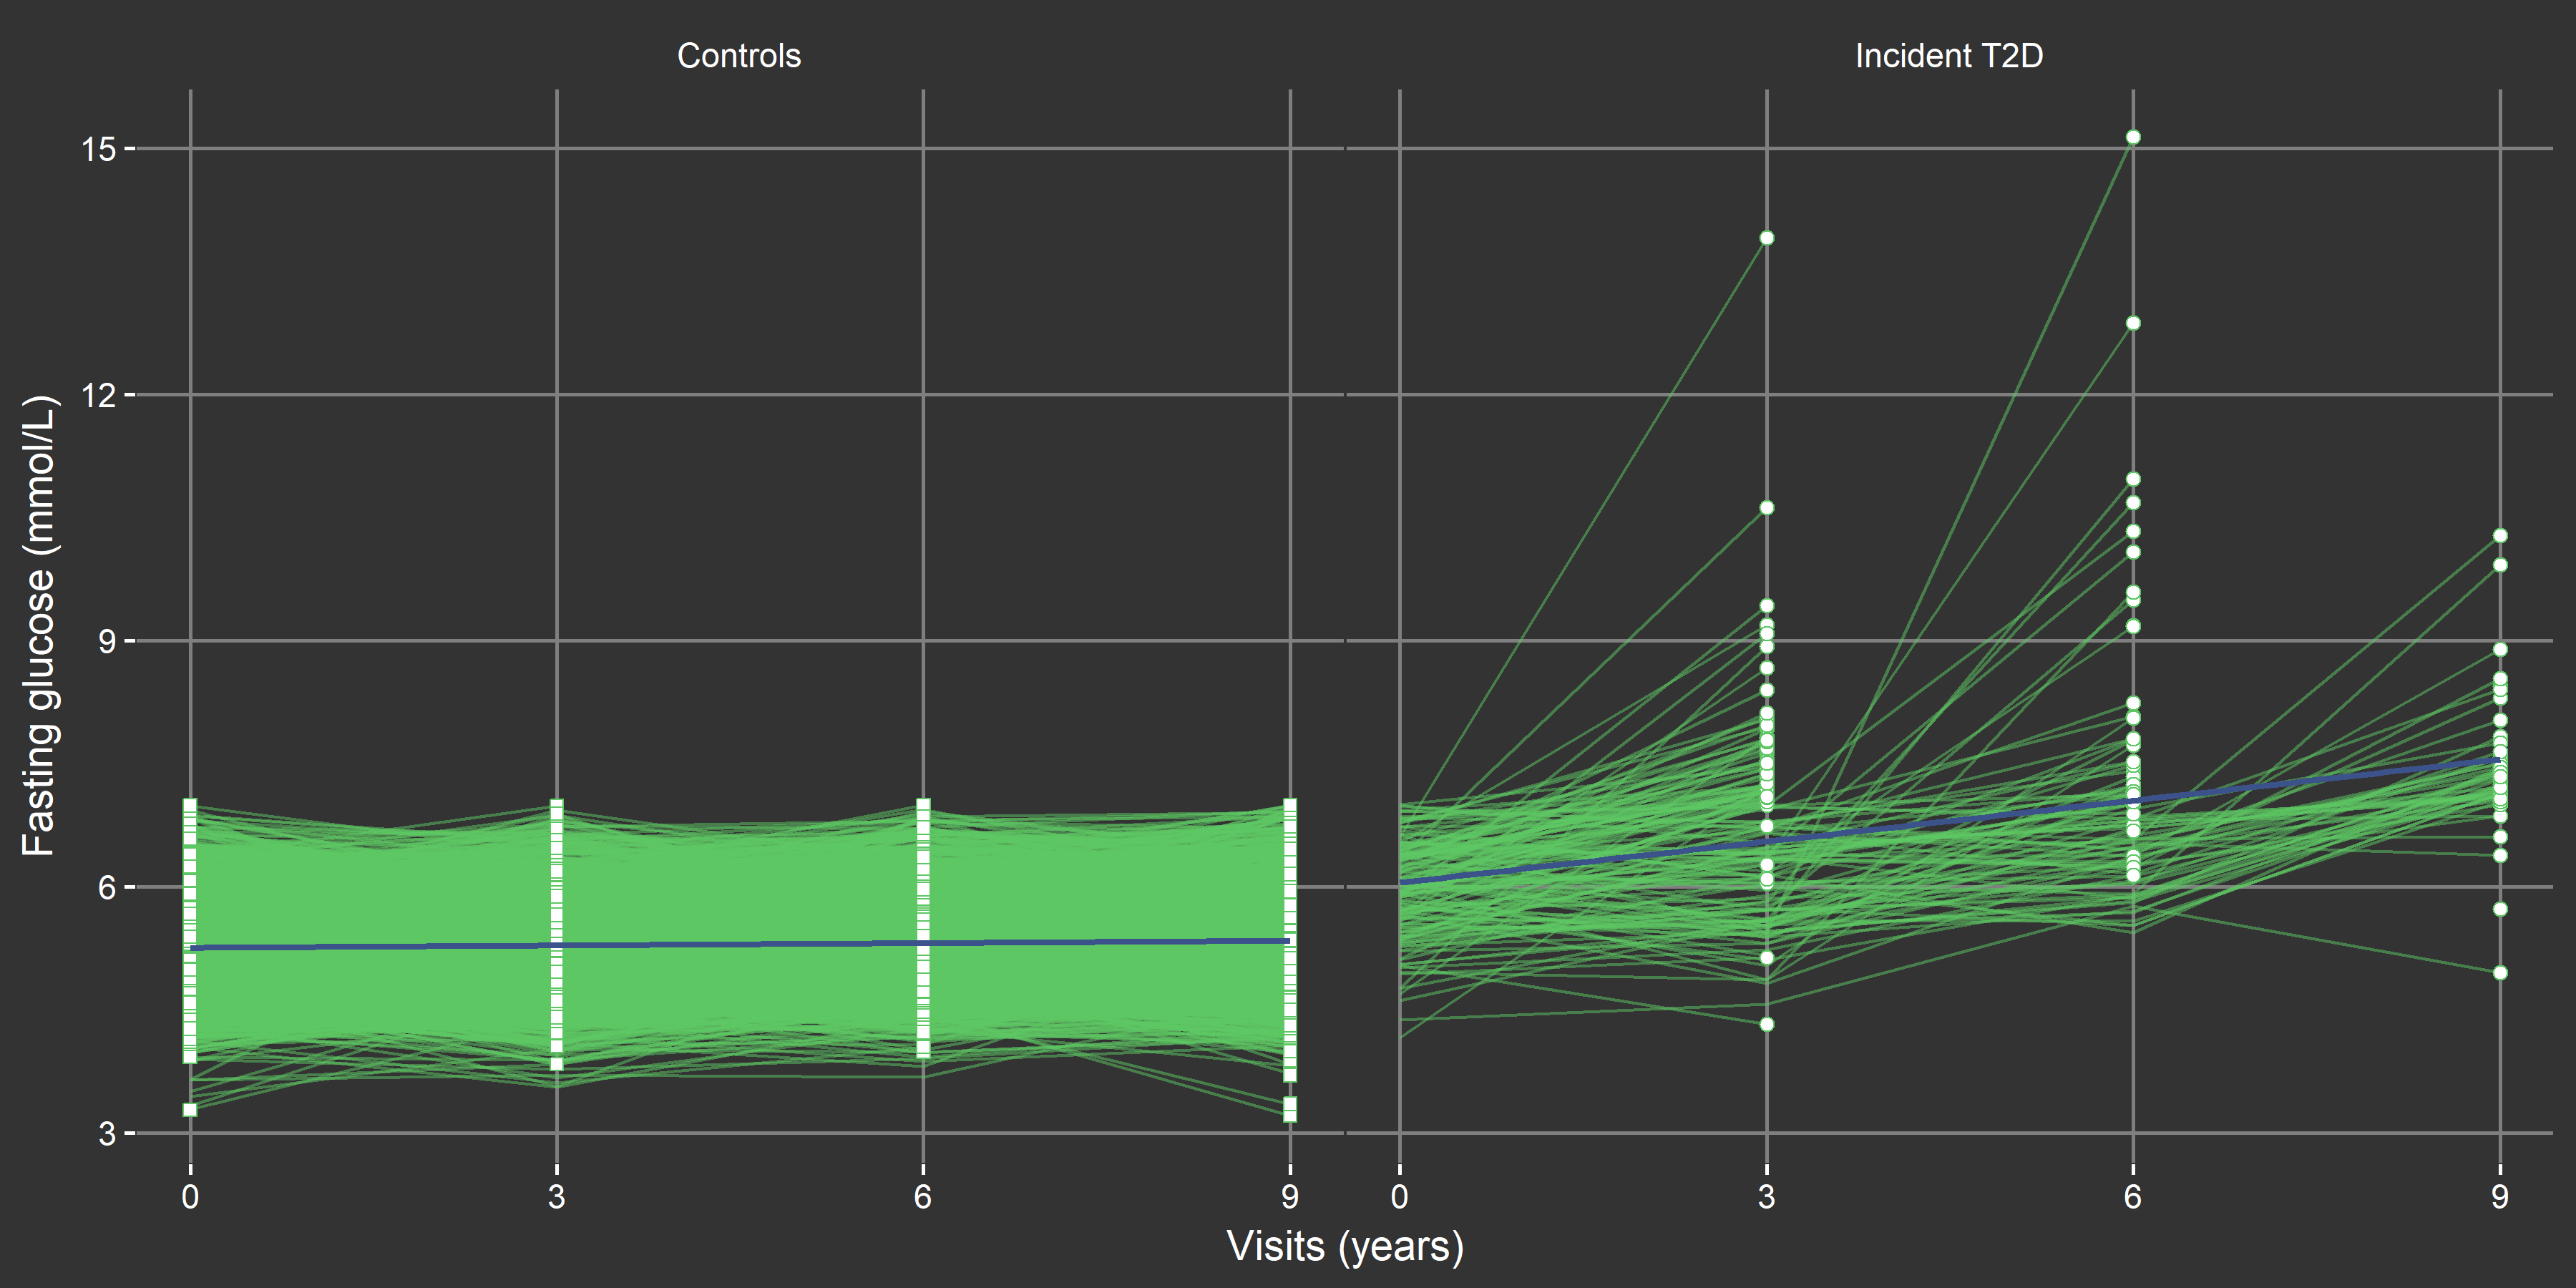
\includegraphics[width=0.95\textwidth]{{images/Fig02.png}}}}
            \captionof{figure}{\color{springgreen3}Trajectoires de la glycémie à jeun des individus D.E.S.I.R.}
        \end{center}
    \end{minipage}
\end{frame}


\begin{frame}{\subsecname}
    \begin{center}
        \alt<2>{\color{black}\fbox{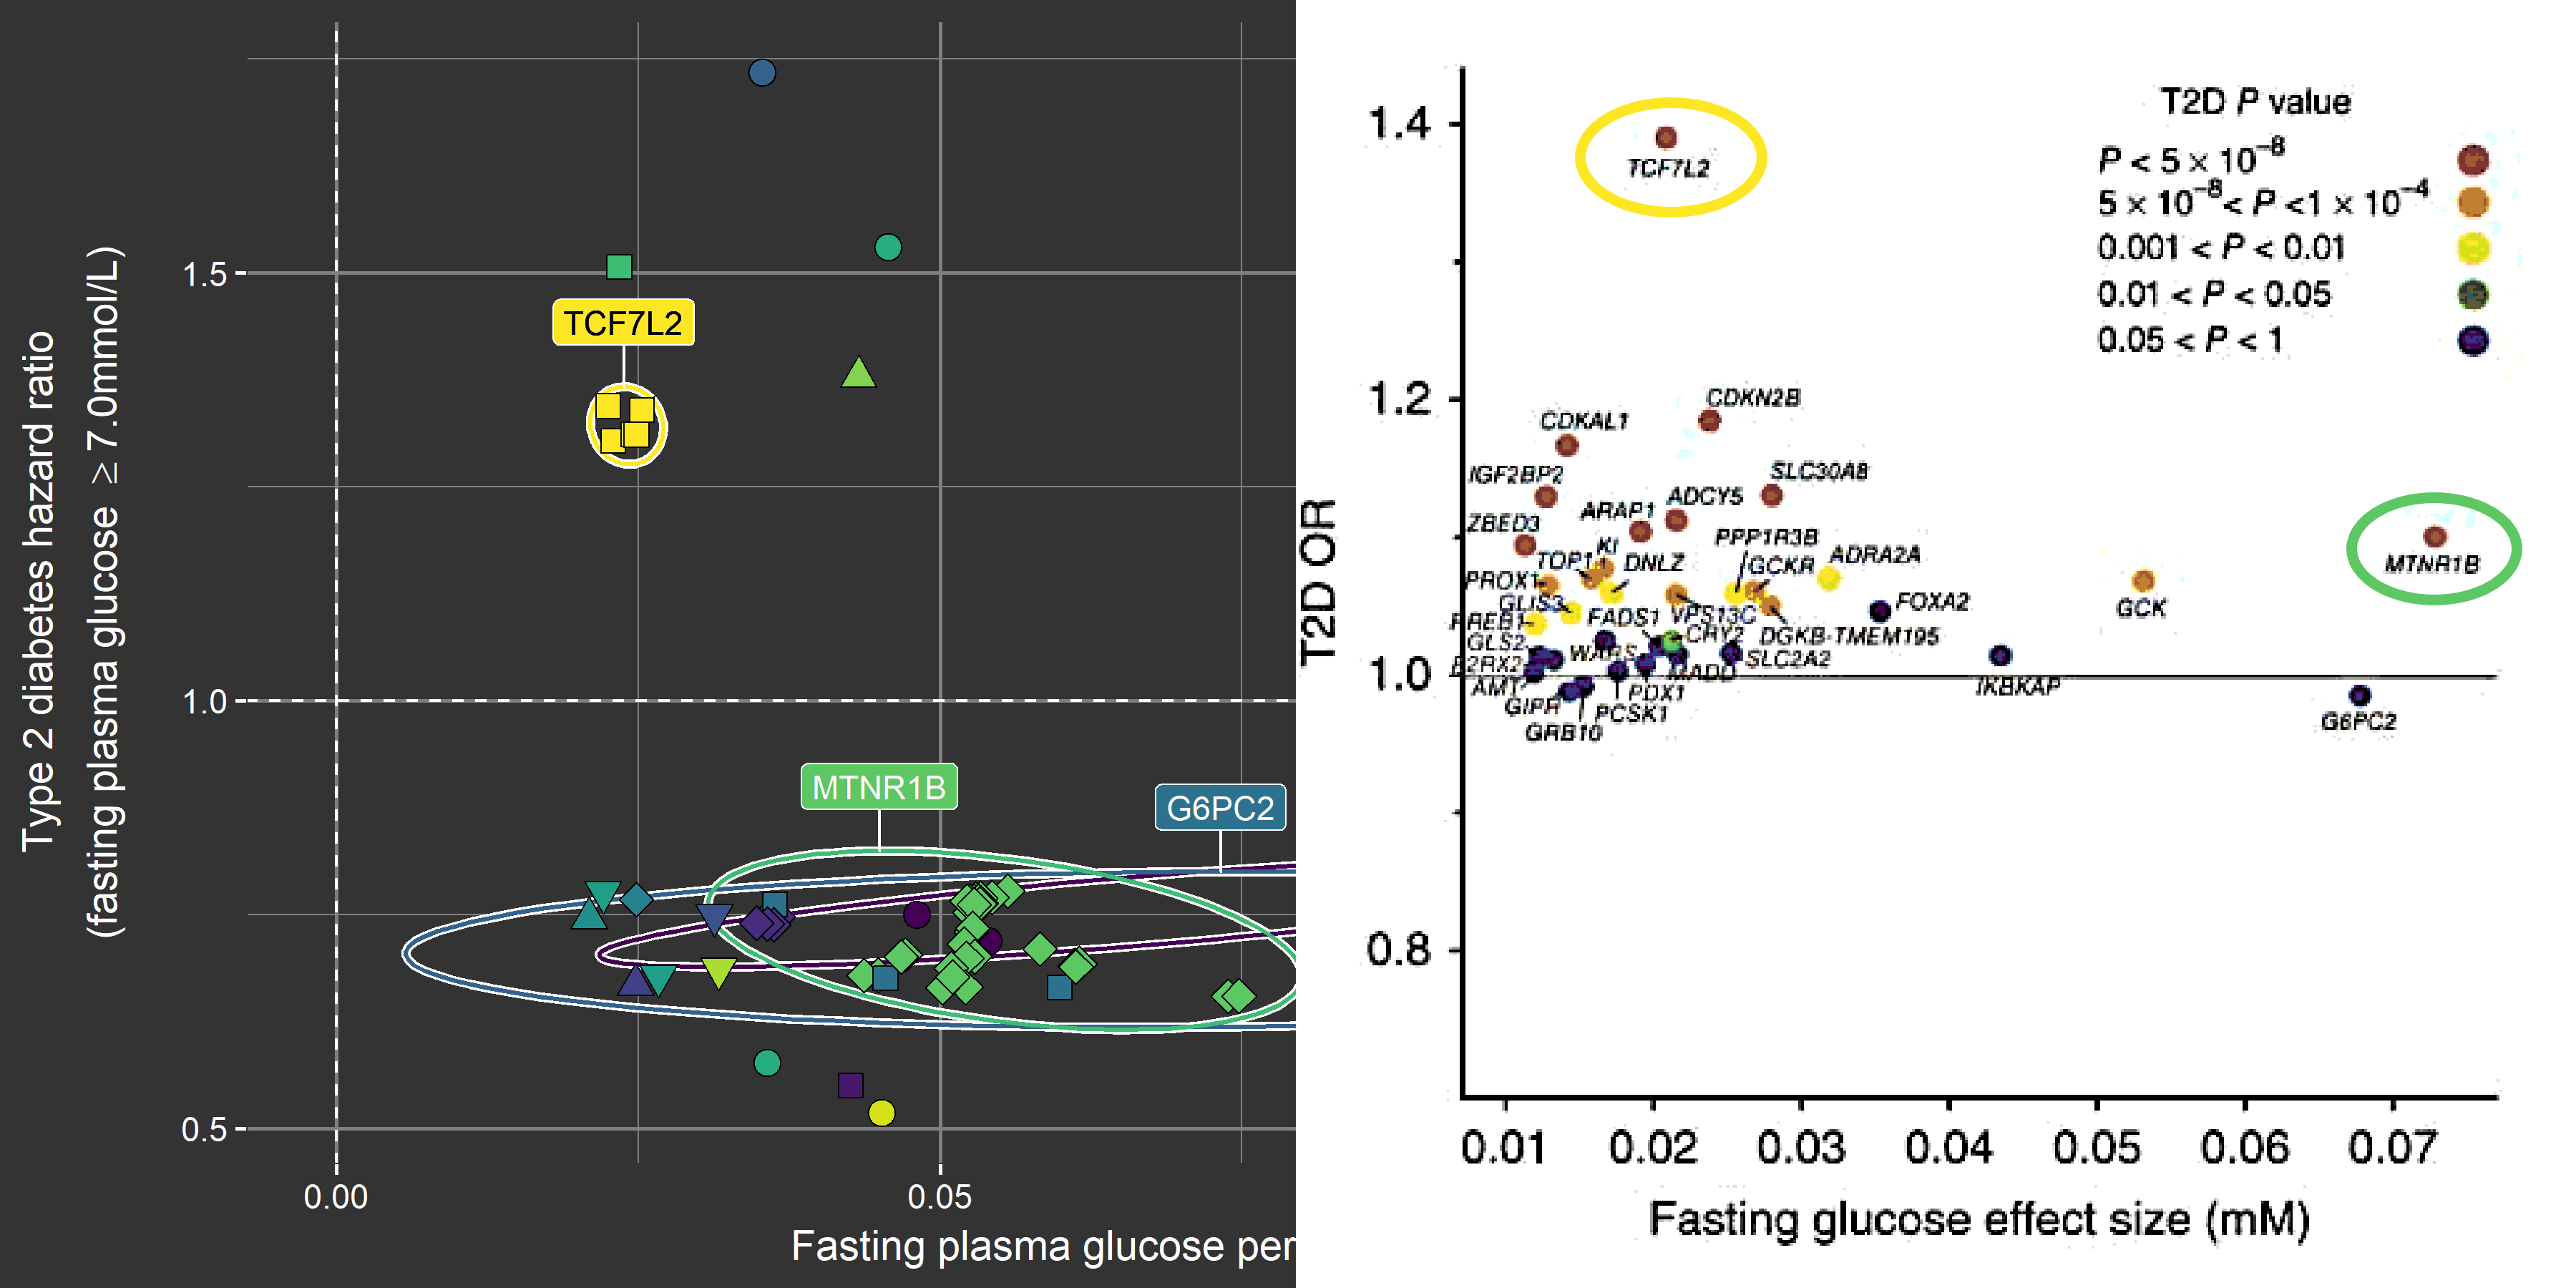
\includegraphics[width=0.95\textwidth]{{images/Fig05b.png}}}}{\color{black}\fbox{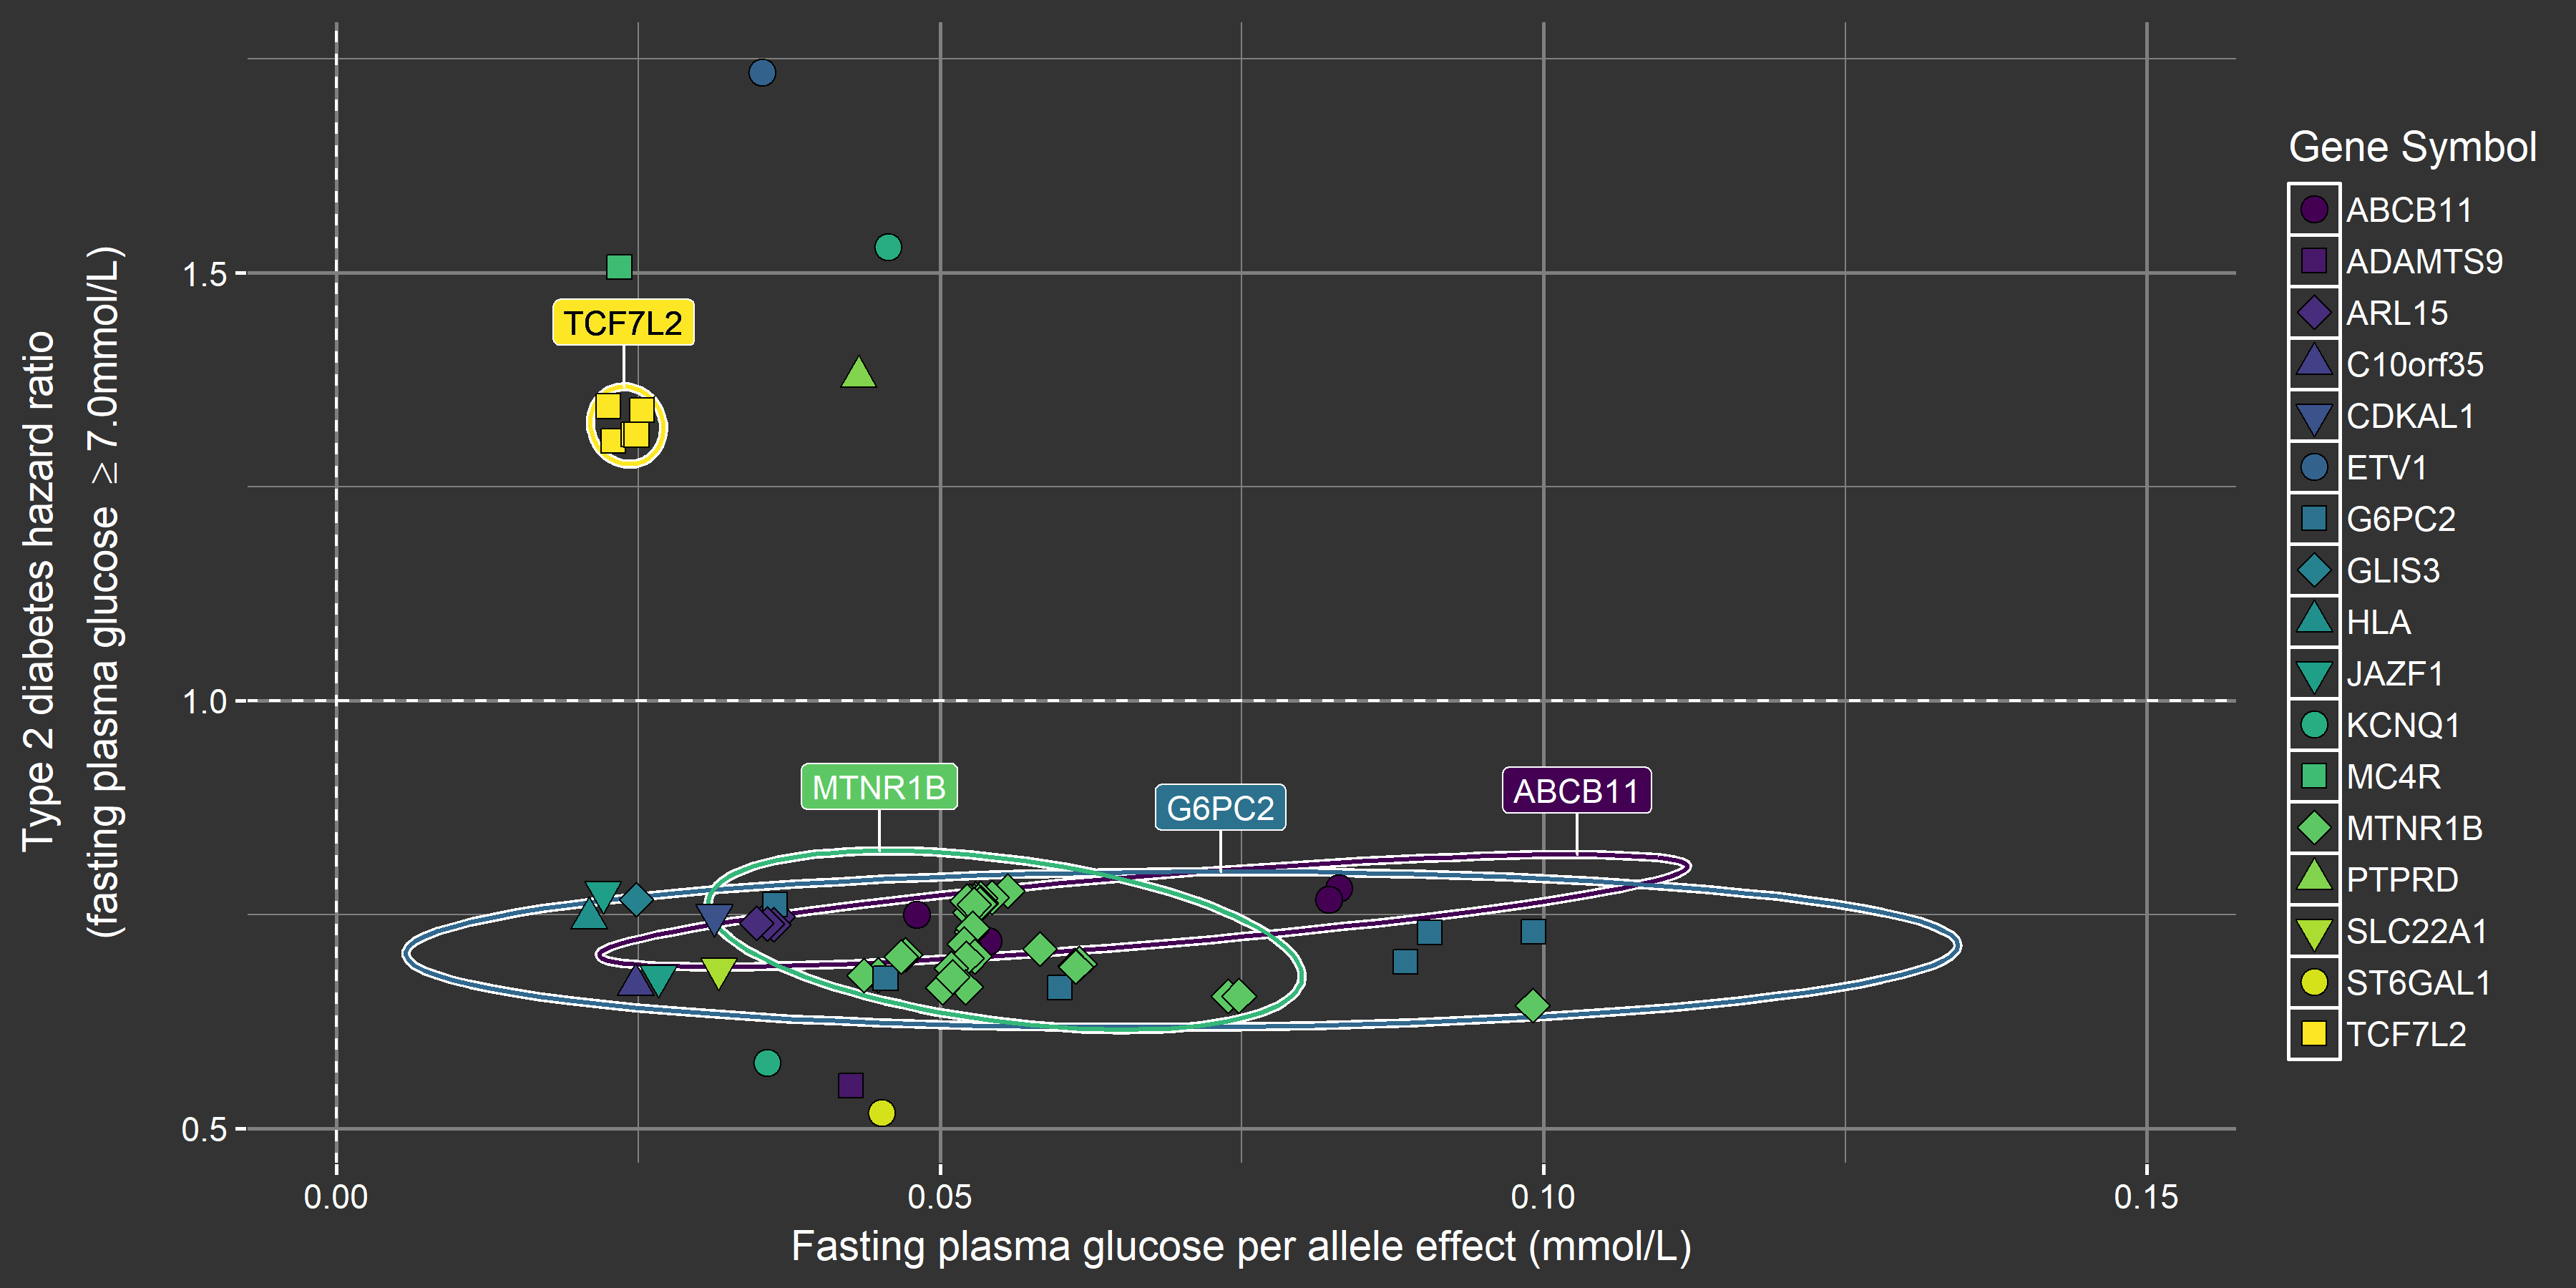
\includegraphics[width=0.95\textwidth]{{images/Fig05.png}}}}
        \captionsetup{labelformat=empty, textfont={bf,it}, width=0.95\textwidth}
        \captionof{figure}{\color{springgreen3}Taille d'effet $\textcolor{springgreen3}{\beta}$ et Hazard Ratio respectivement pour la glycémie et le diabète de type 2. Gènes identifiés dans des études \mbox{pangénomiques} pour une association à la glycémie et/ou au diabète de type 2.}
    \end{center}
\end{frame}


\begin{frame}{\subsecname}
    \everymath{\color{black}}
    \begin{center}
        \begin{table}
            {\fontsize{8pt}{12pt}\selectfont
                \begin{tabular}{cccc}
                    \hline
                    \multirow{2}{*}{SNP (gène)} & \multicolumn{2}{c}{$\beta$ (p-valeur)}\\
                    & JM (D.E.S.I.R.) & TS (D.E.S.I.R.)\\
                    \hline
                    rs10830963\_G (MTNR1B) & $3,25$ ($3,6\times 10^{-42}$) & $3,52$ ($2,7\times 10^{-54}$)\\
                    rs17747324\_C (TCF7L2) & $3,17$ ($8,9\times 10^{-42}$) & $3,39$ ($2,2\times 10^{-52}$)\\
                    \hline
                \end{tabular}
            }
            \captionsetup{labelformat=empty, textfont={bf,it}, width=0.5\textwidth}
            \captionof{table}{\color{springgreen3}Coefficients $\color{springgreen3}\beta$ estimés par JM et TS.}
        \end{table}
    \end{center}
    \everymath{\color{dodgerblue}}
\end{frame}


\begin{frame}{\subsecname}
    \everymath{\color{black}}
    \begin{center}
        \begin{table}
            {\fontsize{8pt}{12pt}\selectfont
                \begin{tabular}{ccccccc}
                    \hline
                    \multirow{2}{*}{SNP (gène)} & \multicolumn{3}{c}{$\gamma$ (p-valeur)}\\
                    & JM (D.E.S.I.R.) & TS (D.E.S.I.R.) & MAGIC\\
                    \hline
                    rs10830963\_G (MTNR1B) & $0,0991$ ($1,3\times 10^{-23}$) & $0,0992$ ($8,9\times 10^{-24}$) & $0,079$ ($1,3\times 10^{-68}$)\\
                    rs17747324\_C (TCF7L2) & $0,0229$ ($3,0\times 10^{-02}$) & $0,0218$ ($3,8\times 10^{-02}$) & $0,025$ ($6,5\times 10^{-08}$)\\
                    \hline
                \end{tabular}
            }
            \captionsetup{labelformat=empty, textfont={bf,it}, width=0.65\textwidth}
            \captionof{table}{\color{springgreen3}Coefficients $\color{springgreen3}\gamma$ estimés par JM et TS, et reportés dans le consortium MAGIC.}
        \end{table}
    	 \begin{table}
            {\fontsize{8pt}{12pt}\selectfont
                \begin{tabular}{ccccccc}
                    \hline
                    \multirow{2}{*}{SNP (gène)} & \multicolumn{3}{c}{$\alpha$ (p-valeur)}\\
                    & JM (D.E.S.I.R.) & TS (D.E.S.I.R.) & DIAGRAM\\
                    \hline
                    rs10830963\_G (MTNR1B) & $-0,440$ ($9,4\times 10^{-04}$) & $-0,443$ ($5,0\times 10^{-04}$) & $0,104$ ($7,3\times 10^{-07}$)\\
                    rs17747324\_C (TCF7L2) & $0,265$ ($4,1\times 10^{-02}$) & $0,284$ ($2,2\times 10^{-02}$) & $0,358$ ($8,5\times 10^{-55}$)\\
                    \hline
                \end{tabular}
            }
            \captionsetup{labelformat=empty, textfont={bf,it}, width=0.65\textwidth}
            \captionof{table}{\color{springgreen3}Coefficients $\color{springgreen3}\alpha$ estimés par JM et TS, et reportés dans le consortium DIAGRAM.}
        \end{table}
    \end{center}
    \everymath{\color{dodgerblue}}
\end{frame}


\subsection{Conclusion: Modèle Joint}
\begin{frame}{\subsecname}
        \begin{center}
            \only<1>{\color{black}\fbox{
\includegraphics[width=\textheight, page=31]{{images/Diagrammes.pdf}}}}%
            \only<2>{\color{black}\fbox{
\includegraphics[width=\textheight, page=32]{{images/Diagrammes.pdf}}}}%
        \end{center}
\end{frame}
%\begin{frame}{\subsecname}
%\begin{itemize}
%\item Cohérence des résultats
%\item Modélisation jointe plus puissante que les approches génétique classique
%\item Temps de calcul important
%\item Approche ``deux-étapes'' comme compromis estimation/temps
%\item[$\Rightarrow$] Soumission en cours dans \textit{Genetic Epidemiolgy}
%\end{itemize}
%\end{frame}
%\note{}


%########################
\section{Au delà des \'Etudes Pangénomiques}
\subsection{Loci de Diabète et Sécrétion d'Insuline}
\begin{frame}{\subsecname}
\begin{center}
 \fcolorbox{black}{white}{
 \begin{minipage}[t]{0.85\columnwidth}\setstretch{1}
 {\normalsize \slshape\bfseries{L'Expression et l'Évaluation Fonctionnelle des Gènes de Susceptibilité au \mbox{Diabète} de Type 2 Identifient Quatre Nouveaux Gènes Contribuant à la Sécrétion \mbox{d'Insuline} Humaine}}\\[0.5em]
{\tiny Fatou K Ndiaye\textsuperscript{1,\textasteriskcentered}, Ana Ortalli\textsuperscript{1,\textasteriskcentered}, \textbf{Mickaël Canouil}\textsuperscript{1,\textasteriskcentered}, Marlène Huyvaert\textsuperscript{1}, Clara Salazar-Cardozo\textsuperscript{1}, Cécile Lecoeur\textsuperscript{1}, Marie Verbanck\textsuperscript{1}, Valérie Pawlowski\textsuperscript{1}, Raphaël Boutry\textsuperscript{1}, Emmanuelle Durand\textsuperscript{1}, Iandry Rabearivelo\textsuperscript{1}, Olivier Sand\textsuperscript{1}, Lorella Marselli\textsuperscript{2}, Julie Kerr-Conte\textsuperscript{3}, Vikash Chandra\textsuperscript{4}, Raphaël Scharfmann\textsuperscript{4}, Odile Poulain-Godefroy\textsuperscript{1}, Piero Marchetti\textsuperscript{2}, François Pattou\textsuperscript{3}, Amar Abderrahmani\textsuperscript{1,5}, Philippe Froguel\textsuperscript{1,5,\textdagger} \& Amélie Bonnefond\textsuperscript{1,5,\textdagger}\\
\textsuperscript{\textasteriskcentered}Co-premier auteurs.\\
\textsuperscript{\textdagger}Co-dernier auteurs.
}
\end{minipage}%
}
\end{center}
\end{frame}

%\begin{frame}{\subsecname: \subsubsecname}
%\vspace{-1em}
%\begin{minipage}[t]{0.475\columnwidth}
%\vspace{1em}
%	\begin{itemize}
%	\item Plus de 100 loci associés au risque de diabète de type 2
%		\begin{itemize}\setlength{\itemindent}{-.15in}
%			\item<2->[$\Rightarrow$] Relation entre l'expression et le diabète de type 2
%			\begin{itemize}\setlength{\itemindent}{-.25in}
%				\item<3->[$\Rightarrow$] Effet sur la sécrétion d'insuline
%			\end{itemize}
%		\end{itemize}
%	\end{itemize}
%\vspace{1em}
%\end{minipage}%
%\hfill\vline\hfill
%\begin{minipage}[t]{0.475\columnwidth}%
%\vspace{3em}
%\begin{center}\begin{minipage}[t]{0.85\textwidth}\vspace{-1.5em}\begin{block}{\itshape\textbf{EndoC $\color{white}\beta$H1}}\setstretch{1}
%\begin{itemize}
%\item Organe: Pancréas
%\item \texttildelow 25 loci étudiés
%\item 4 nouveaux loci impliqués dans la sécrétion d'insuline
%\end{itemize}
%\end{block}\vspace{1.5em}\end{minipage}\end{center}
%\vspace{1em}
%\end{minipage}
%\end{frame}
%\note{}


\begin{frame}{\subsecname}
       \begin{center}
            \only<1>{\color{black}\fbox{
\includegraphics[width=\textheight, page=11]{{images/Diagrammes.pdf}}}}%
            \only<2>{\color{black}\fbox{
\includegraphics[width=\textheight, page=12]{{images/Diagrammes.pdf}}}}%
            \only<3>{\color{black}\fbox{
\includegraphics[width=\textheight, page=13]{{images/Diagrammes.pdf}}}}%
            \only<4>{\color{black}\fbox{
\includegraphics[width=\textheight, page=14]{{images/Diagrammes.pdf}}}}%
            \only<5>{\color{black}\fbox{
\includegraphics[width=\textheight, page=15]{{images/Diagrammes.pdf}}}}%
            \only<6>{\color{black}\fbox{
\includegraphics[width=\textheight, page=16]{{images/Diagrammes.pdf}}}}%
            \only<7>{\color{black}\fbox{
\includegraphics[width=\textheight, page=17]{{images/Diagrammes.pdf}}}}%
            \only<8>{\color{black}\fbox{
\includegraphics[width=\textheight, page=18]{{images/Diagrammes.pdf}}}}%
            \only<9>{\color{black}\fbox{
\includegraphics[width=\textheight, page=19]{{images/Diagrammes.pdf}}}}%
            \only<10>{\color{black}\fbox{
\includegraphics[width=\textheight, page=20]{{images/Diagrammes.pdf}}}}%
            \only<11>{\color{black}\fbox{
\includegraphics[width=\textheight, page=21]{{images/Diagrammes.pdf}}}}%
            \only<12>{\color{black}\fbox{
\includegraphics[width=\textheight, page=22]{{images/Diagrammes.pdf}}}}%
        \end{center}
\end{frame}


\subsection{Méthylation et Expression: le Cas de PDGFA}
\begin{frame}{\subsecname}
\begin{center}
 \fcolorbox{black}{white}{
 \begin{minipage}[t]{0.85\columnwidth}\setstretch{1}
 {\normalsize \slshape\bfseries{La Surexpression Hépatique de PDGF-AA Affaiblit la Signalisation de l'Insuline dans le Diabète}}\\[0.5em]
{\tiny Amar Abderrahmani\textsuperscript{1,2\textasteriskcentered}, Loïc Yengo\textsuperscript{1\textasteriskcentered}, Robert Caiazzo\textsuperscript{3\textasteriskcentered}, \textbf{Mickaël Canouil}\textsuperscript{1\textasteriskcentered}, Stéphane Cauchi\textsuperscript{1}, Violeta Raverdy\textsuperscript{2}, Valérie Plaisance\textsuperscript{1}, Stéphane Lobbens\textsuperscript{1}, Julie Maillet\textsuperscript{1}, Laure Rolland\textsuperscript{1}, Raphael Boutry\textsuperscript{1}, Maxime Kwapich\textsuperscript{1}, Mathie Tenenbaum\textsuperscript{1}, Julien Bricambert\textsuperscript{1}, Sophie Saussenthaler\textsuperscript{4}, Elodie Anthony\textsuperscript{5}, Pooja Jha\textsuperscript{6}, Julien Derop\textsuperscript{1}, Olivier Sand\textsuperscript{1}, Iandry Rabearivelo\textsuperscript{1}, Audrey Leloire\textsuperscript{1}, Marie Pigeyre\textsuperscript{2}, Martine Daujat-Chavanieu\textsuperscript{7}, Sabine Gerbal-Chaloin\textsuperscript{7}, Tasnim Dayeh\textsuperscript{8}, Guillaume Lassailly\textsuperscript{2}, Philippe Mathurin\textsuperscript{9}, Bart Staels\textsuperscript{10}, Johan Auwerx\textsuperscript{5}, Annette Schürmann\textsuperscript{4}, Catherine Postic\textsuperscript{5}, Clemens Schafmayer\textsuperscript{11}, Jochen Hampe\textsuperscript{12}, Amélie Bonnefond\textsuperscript{1,2}, François Pattou\textsuperscript{3\textdagger} \& Philippe Froguel\textsuperscript{1,2\textdagger}\\
\textsuperscript{\textasteriskcentered}Co-premier auteurs.\\
\textsuperscript{\textdagger}Co-dernier auteurs. 
}
\end{minipage}%
}
\end{center}
\end{frame}


\begin{frame}{\subsecname}
        \begin{center}
            \only<1>{\color{black}\fbox{
\includegraphics[width=\textheight, page=1]{{images/Diagrammes.pdf}}}}%
            \only<2>{\color{black}\fbox{
\includegraphics[width=\textheight, page=2]{{images/Diagrammes.pdf}}}}%
            \only<3>{\color{black}\fbox{
\includegraphics[width=\textheight, page=3]{{images/Diagrammes.pdf}}}}%
            \only<4>{\color{black}\fbox{
\includegraphics[width=\textheight, page=4]{{images/Diagrammes.pdf}}}}%
            \only<5>{\color{black}\fbox{
\includegraphics[width=\textheight, page=5]{{images/Diagrammes.pdf}}}}%
            \only<6>{\color{black}\fbox{
\includegraphics[width=\textheight, page=6]{{images/Diagrammes.pdf}}}}%
            \only<7>{\color{black}\fbox{
\includegraphics[width=\textheight, page=7]{{images/Diagrammes.pdf}}}}%
            \only<8>{\color{black}\fbox{
\includegraphics[width=\textheight, page=8]{{images/Diagrammes.pdf}}}}%
            \only<9>{\color{black}\fbox{
\includegraphics[width=\textheight, page=9]{{images/Diagrammes.pdf}}}}%
            \only<10>{\color{black}\fbox{
\includegraphics[width=\textheight, page=10]{{images/Diagrammes.pdf}}}}%
        \end{center}
\end{frame}


%\begin{frame}{\subsecname: \subsubsecname}
%\vspace{-1em}
%\begin{minipage}[t]{0.475\columnwidth}
%\vspace{1em}
%\begin{center}\begin{minipage}[t]{0.85\textwidth}\vspace{-1.5em}\begin{block}{\itshape\textbf{A.B.O.S.}}\setstretch{1}
%{\small\begin{itemize}\setlength{\itemindent}{-0.1in}
%\item Atlas Biologique de l'Obésité Sévère
%\item Organe: Foie
%\item 192 femmes obèse
%\item Illumina HumanMethylation 450K $\Rightarrow$ Méthylation
%\item Illumina HT-12 $\Rightarrow$ Expression
%\end{itemize}}
%\end{block}\vspace{1em}\end{minipage}\end{center}
%\begin{itemize}
%	\item<2-> Tests multiples
%	\only<3>{\item[$\Rightarrow$] Correction du seuil $\alpha$:\\p. ex. Bonferroni: $\tilde{\alpha}=\frac{\alpha}{N_{test}}$}
%	\item<4-> Inflation des valeurs-p
%	\only<5>{\item[$\Rightarrow$] Correction par le facteur d'inflation: \mbox{$\lambda=\frac{median(\chi^2_1, \cdots, \chi^2_m)}{0,4559}$}}
%\end{itemize}
%\end{minipage}%
%\hfill\vline\hfill
%\begin{minipage}[t]{0.475\columnwidth}%
%	\vspace{1em}
%        \begin{center}
%            {\color{black}\fbox{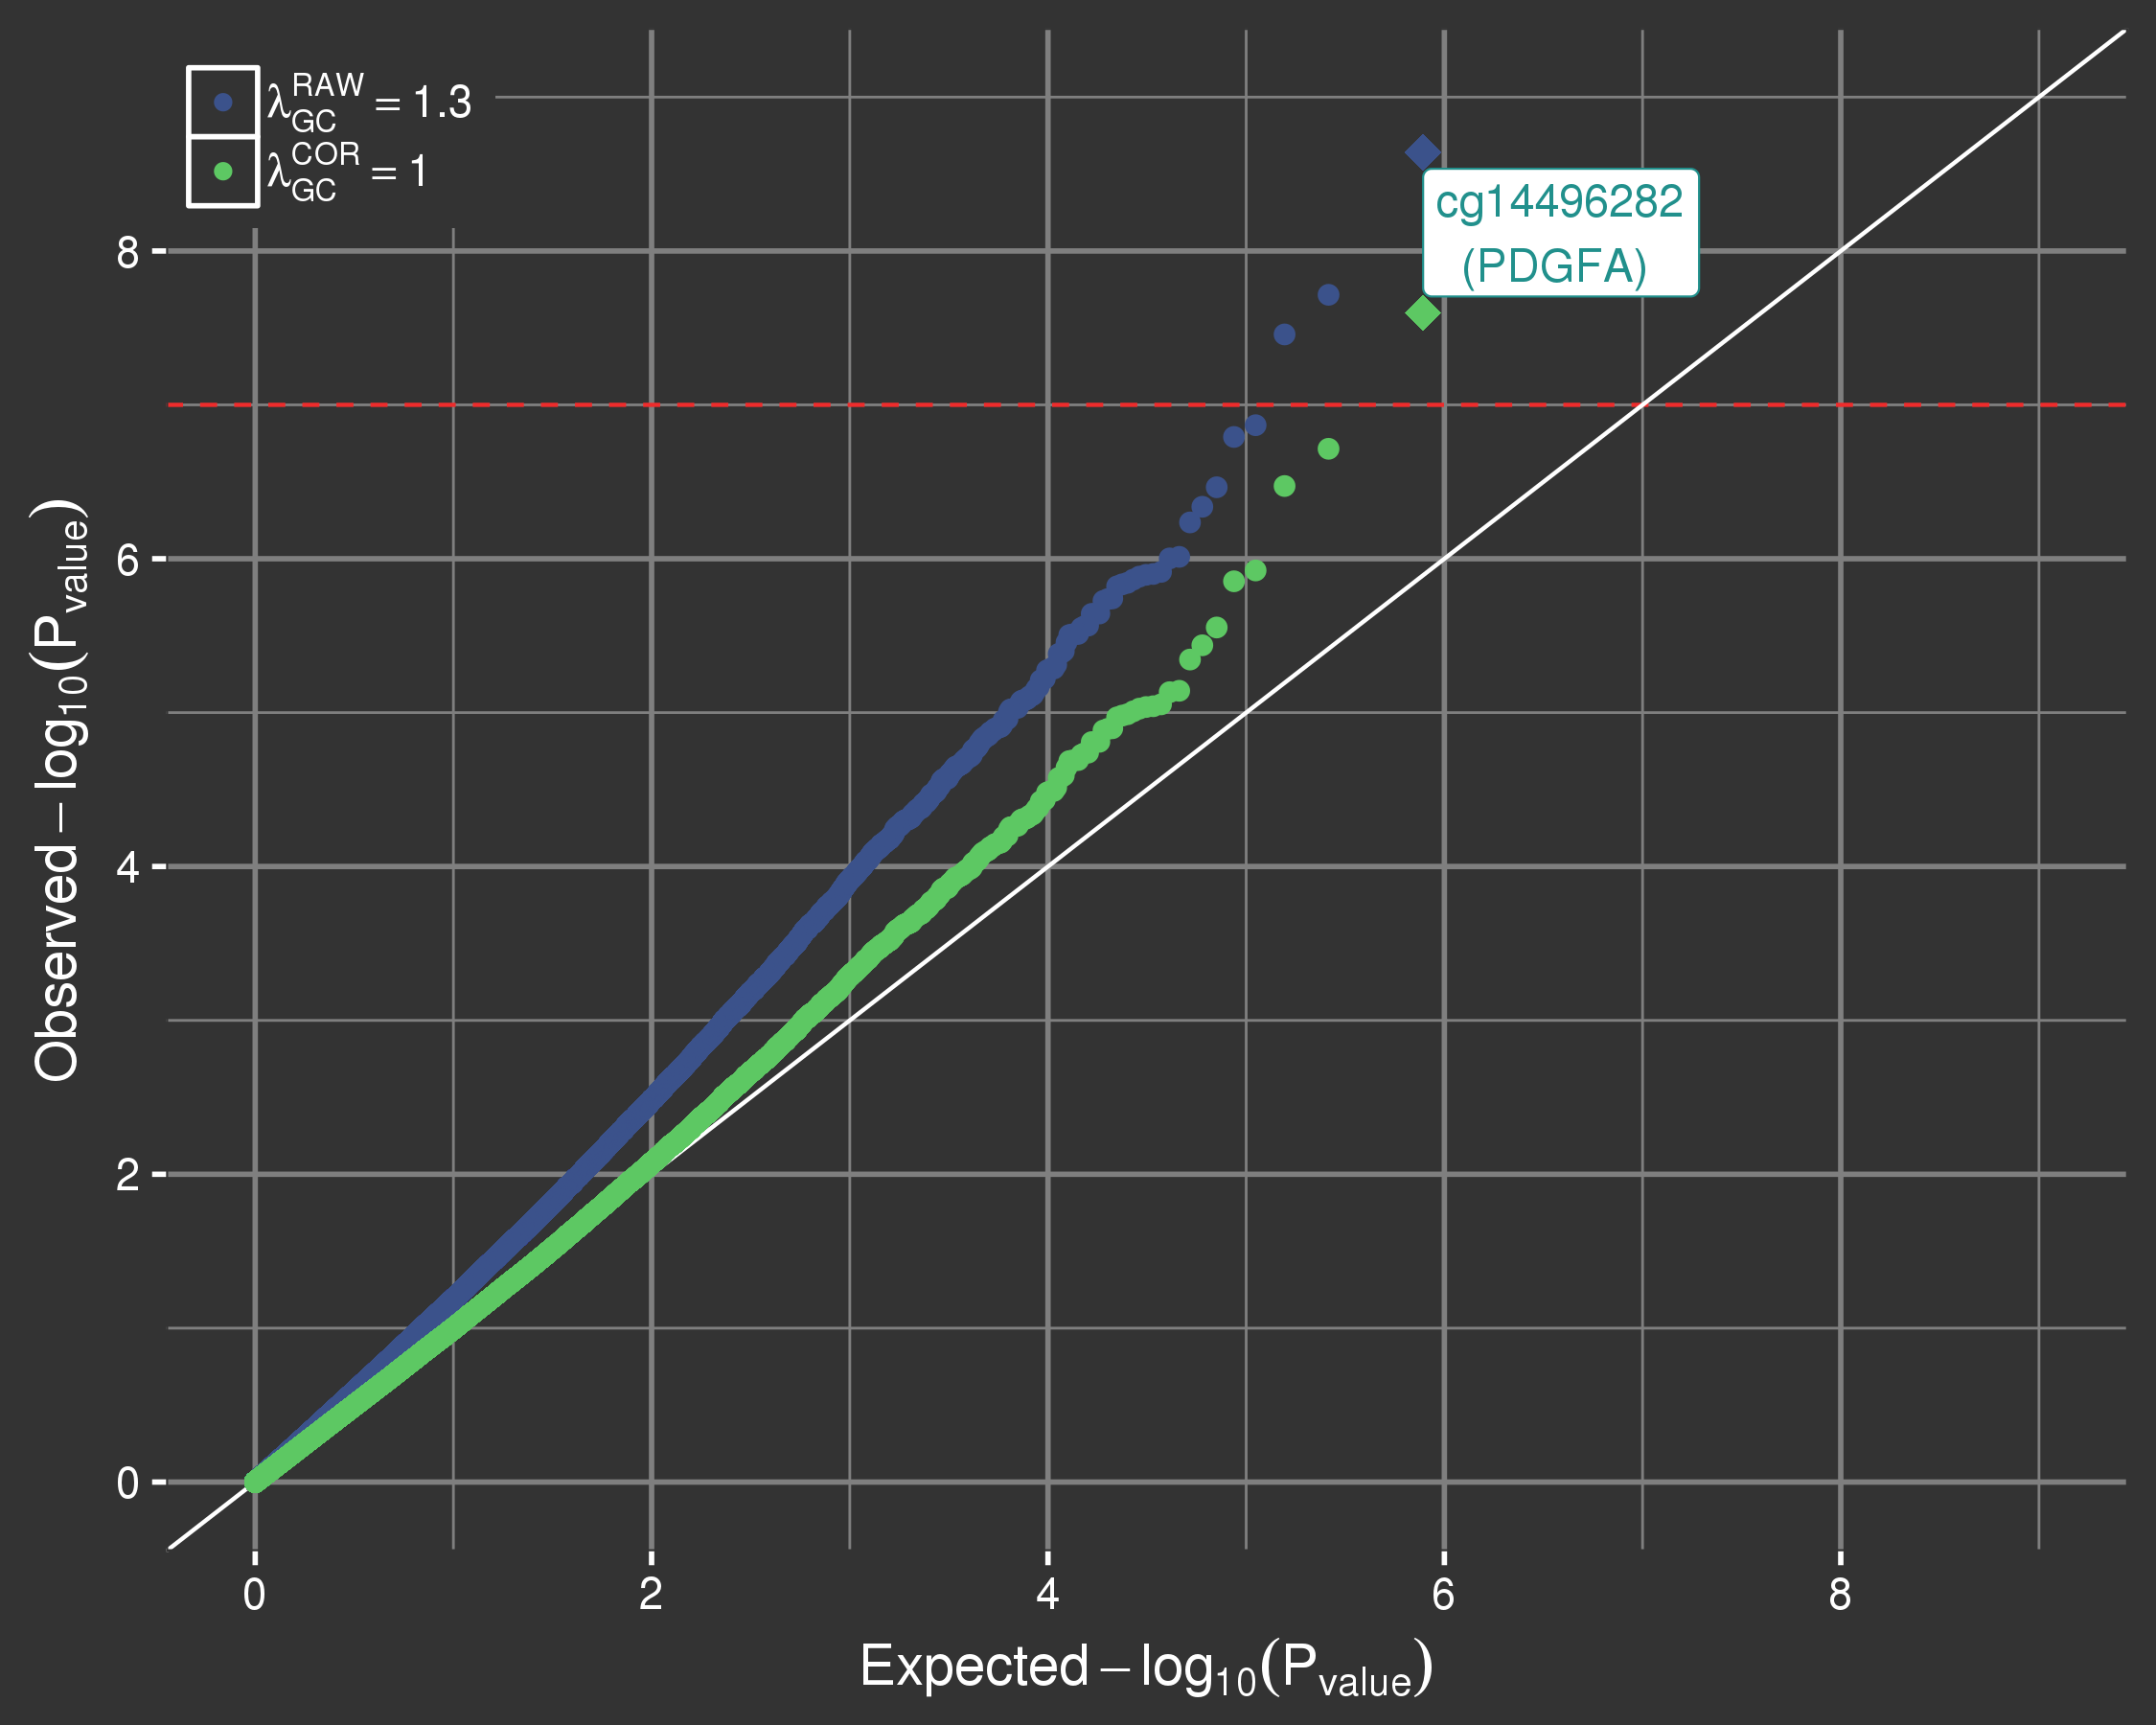
\includegraphics[width=5cm]{{images/Fig29.png}}}}
%            \captionof{figure}{\color{springgreen3}Graphique quantile-quantile des valeurs-p de l'étude
%d'association épigénétique en cas/contrôle sur le diabète de type 2}
%        \end{center}
%        \vspace{1em}
%\end{minipage}
%\end{frame}
%\note{
%Une correction appelée contrôle génomique (``Genomic control'') peut être appliquée, avec comme principale motivation la correction d'une éventuelle stratification ou mélange au sein de la population d'étude. 
%Cette inflation est mesurée par le paramètre de sur-dispersion $\lambda$ sur l'ensemble des statistiques de test observées \citep{devlin_genomic_1999}. 
%Il est estimé à partir de la distribution observée des m statistiques de test de chi-deux comparée à celle attendue sous l'hypothèse nulle. 
%Pour se prémunir des valeurs extrêmes, la valeur médiane (et non la moyenne) est utilisée $\lambda=\frac{median(\chi^2_1, \cdots, \chi^2_m)}{0,4549}$.
%La distribution de la statistique de test observée dans l'étude est ensuite corrigée par ce facteur $\lambda$.
%Il est à noter que même si le paramètre $\lambda$ n'est pas directement relié à la fréquence allélique, cette correction peut toutefois engendrer une perte de puissance \citep{georgiopoulos_power_2016}
%}


%\begin{frame}{\subsecname: \subsubsecname}
%\vspace{-1em}
%\begin{minipage}[t]{0.475\columnwidth}
%\vspace{1em}
%        \begin{center}
%            {\color{black}\fbox{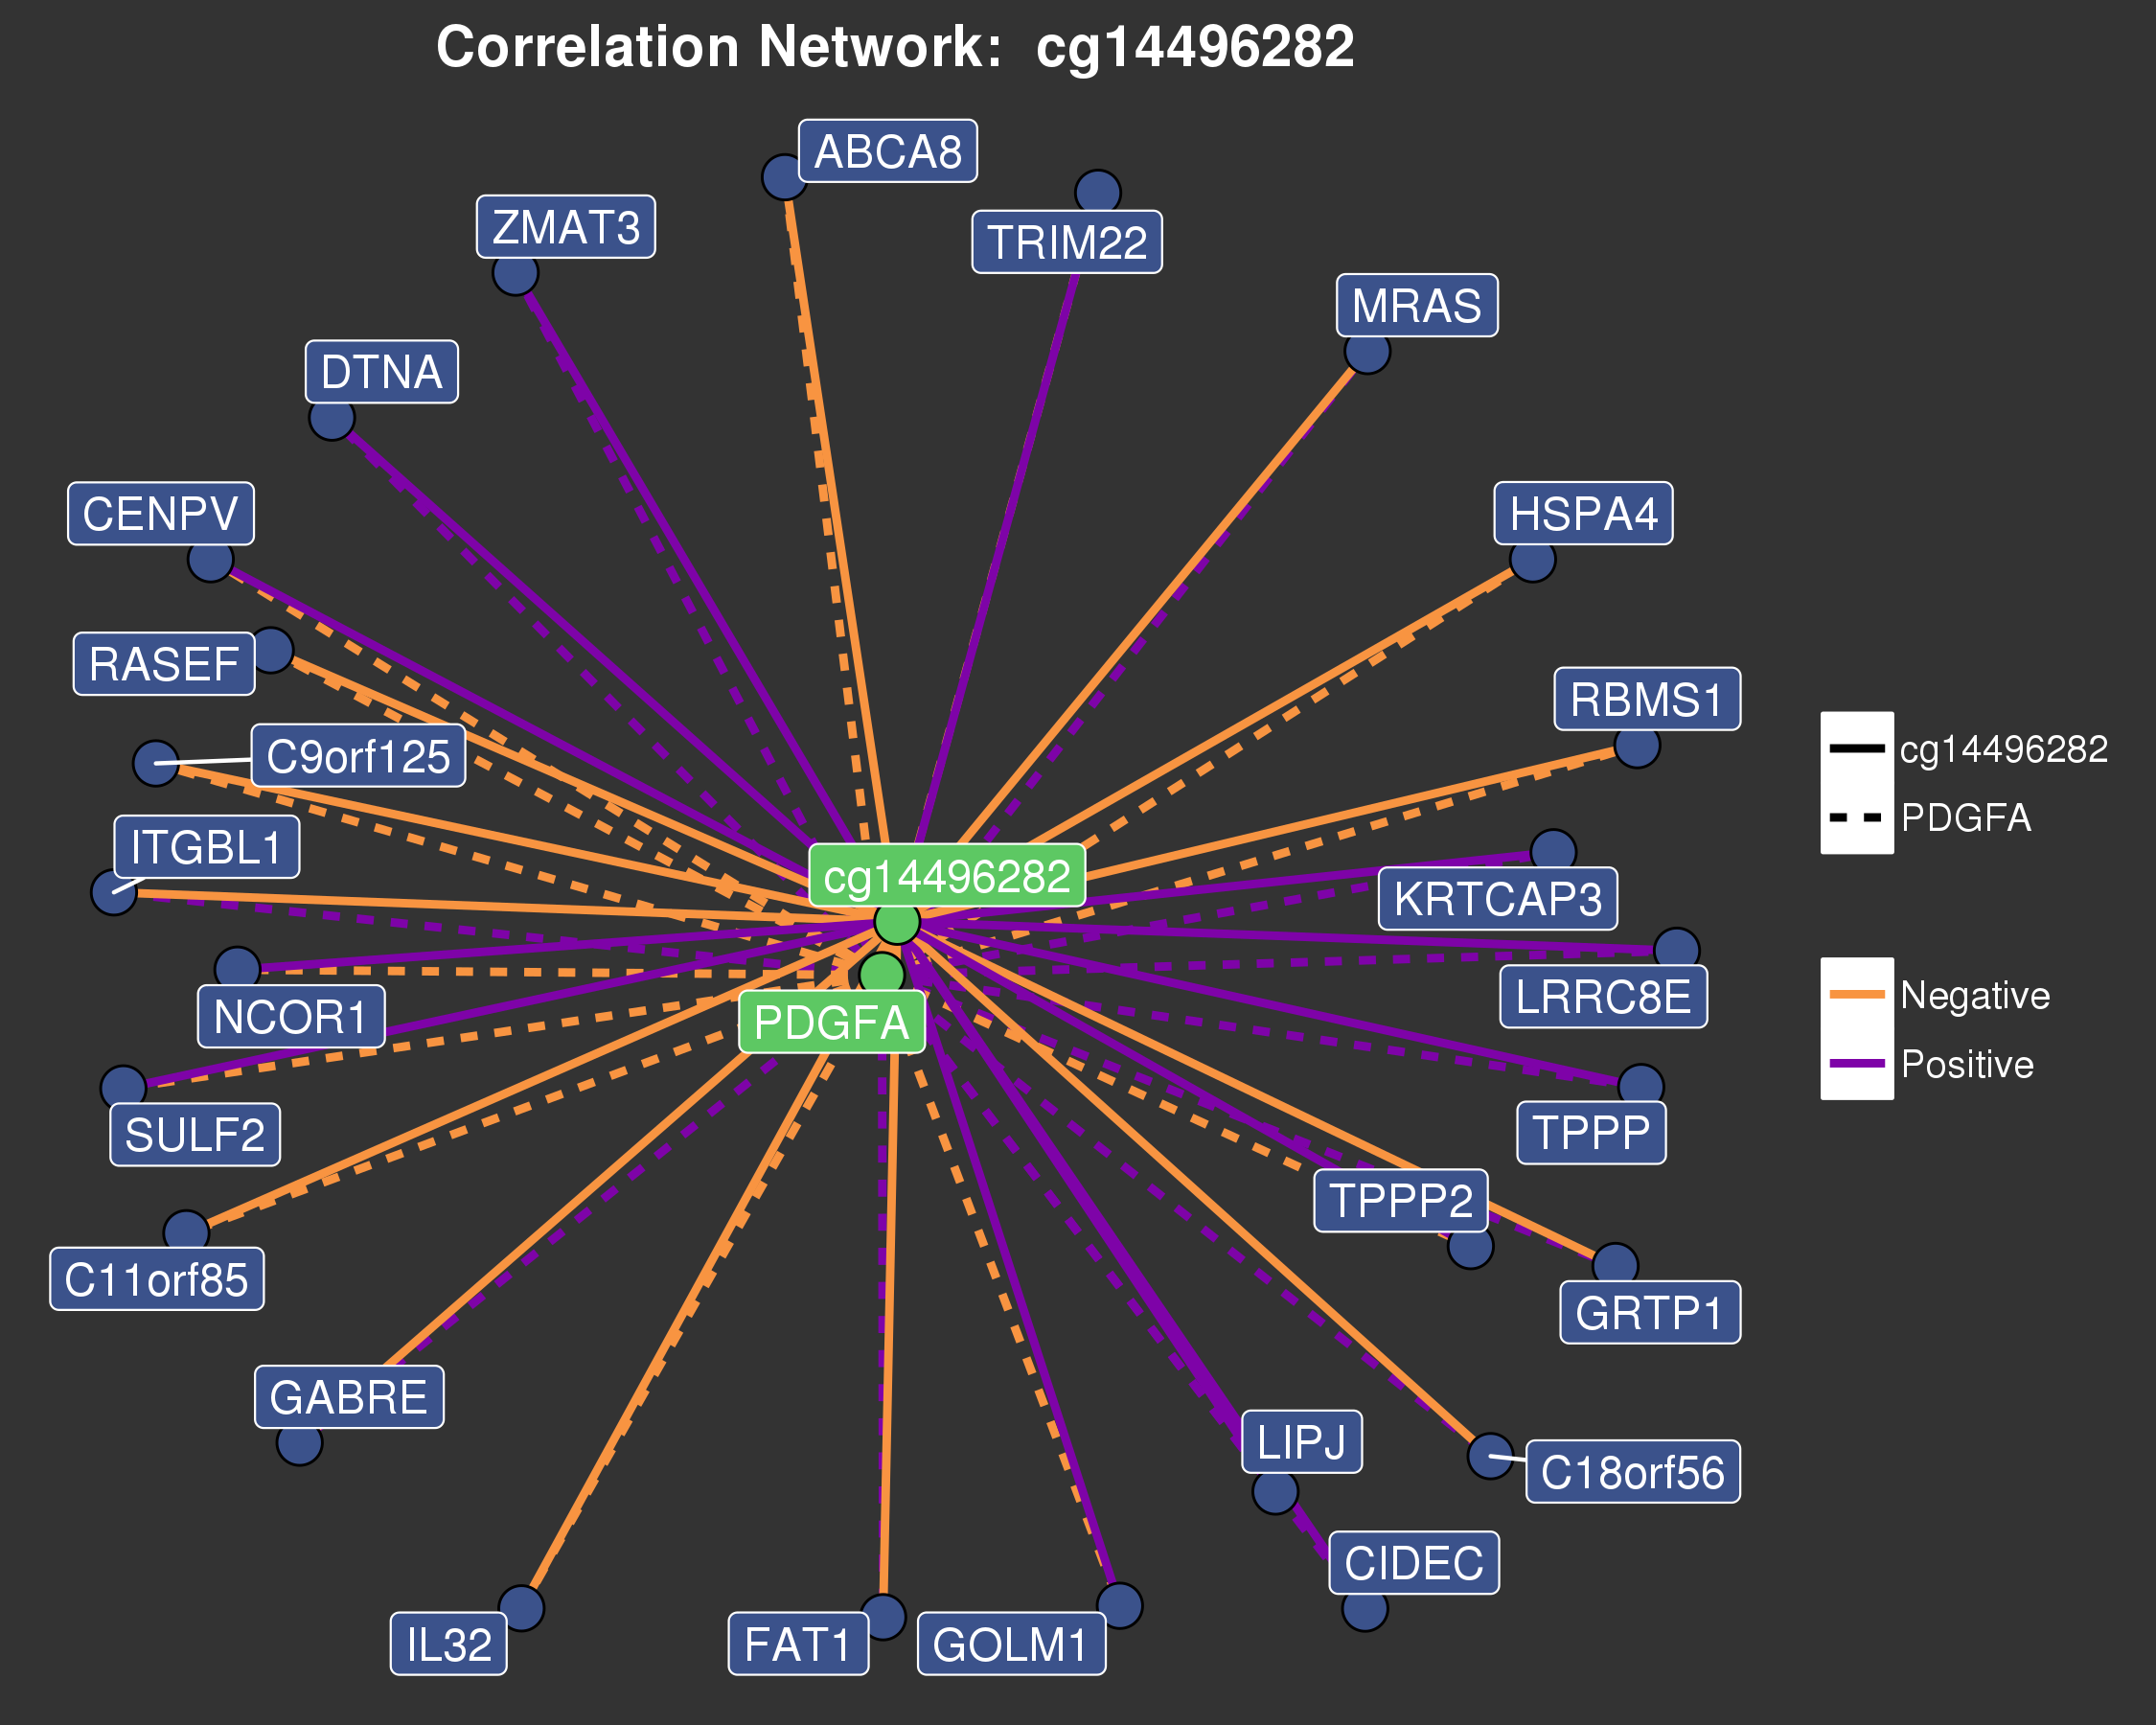
\includegraphics[width=5cm]{{images/Fig31.png}}}}
%            \captionof{figure}{\color{springgreen3}Réseau de corrélation autour du site CpG et du gène PDGFA.}
%        \end{center}
%        \vspace{1em}
%\end{minipage}%
%\hfill\vline\hfill
%\begin{minipage}[t]{0.475\columnwidth}%
%\vspace{3em}
%\begin{itemize}
%\item cg14496282 associé au diabète de type 2
%\item Corrélation inverse de la méthylation et l'expression
%\item Association entre l'insulinémie (GRS) et la méthylation 
%\end{itemize}
%\vspace{1em}
%\end{minipage}
%\end{frame}
%\note{}


\subsection{Méthylation et Expression: le Bisphénol et ses Substituants}
\begin{frame}{\subsecname}
\begin{center}
 \fcolorbox{black}{white}{
 \begin{minipage}[t]{0.85\columnwidth}\setstretch{1}
 {\normalsize \slshape\bfseries{L'Exposition à Faible Dose aux Bisphénols A, F et S des Adipocytes Primaires \mbox{Humains} Modifie les Profils d'ARN Codant et Non-Codant}}\\[0.5em]
{\tiny Marie Verbanck\textsuperscript{1,\textasteriskcentered}, \textbf{Mickaël Canouil}\textsuperscript{1,\textasteriskcentered}, Audrey Leloire\textsuperscript{1}, Véronique Dhennin\textsuperscript{1}, Xavier
Coumoul\textsuperscript{2}, Loïc Yengo\textsuperscript{1}, Philippe Froguel\textsuperscript{1,3,\textdagger} \& Odile Poulain-Godefroy\textsuperscript{1,\textdagger}\\
\textsuperscript{\textasteriskcentered}Co-premier auteurs.\\
\textsuperscript{\textdagger}Co-dernier auteurs. 
}
\end{minipage}%
}
\end{center}
\end{frame}


\begin{frame}{\subsecname}
        \begin{center}
            \only<1>{\color{black}\fbox{
\includegraphics[width=\textheight, page=23]{{images/Diagrammes.pdf}}}}%
            \only<2>{\color{black}\fbox{\includegraphics[width=\textheight, page=24]{{images/Diagrammes.pdf}}}}%
            \only<3>{\color{black}\fbox{\includegraphics[width=\textheight, page=25]{{images/Diagrammes.pdf}}}}%
            \only<4>{\color{black}\fbox{\includegraphics[width=\textheight, page=26]{{images/Diagrammes.pdf}}}}%
            \only<5>{\color{black}\fbox{\includegraphics[width=\textheight, page=27]{{images/Diagrammes.pdf}}}}%
            \only<6>{\color{black}\fbox{\includegraphics[width=\textheight, page=28]{{images/Diagrammes.pdf}}}}%
            \only<7>{\color{black}\fbox{\includegraphics[width=\textheight, page=29]{{images/Diagrammes.pdf}}}}%
            \only<8>{\color{black}\fbox{\includegraphics[width=\textheight, page=30]{{images/Diagrammes.pdf}}}}%
        \end{center}
\end{frame}


%\begin{frame}{\subsecname: \subsubsecname}
%
%        \begin{center}
%            {\color{black}\fbox{\includegraphics[width=8cm]{{images/schemaDesign.png}}}}
%            \captionof{figure}{\color{springgreen3}Schéma de l'étude de polluants dans des adipocytes.}
%        \end{center}
%\end{frame}
%\note{}
%
%\begin{frame}{\subsecname: \subsubsecname}
%\vspace{-1em}
%\begin{minipage}[t]{0.475\columnwidth}
%\vspace{1em}
%        \begin{center}
%            {\color{black}\fbox{\includegraphics[width=5cm]{{images/Fig32.png}}}}
%            \captionof{figure}{\color{springgreen3}Heatmap de l'expression de gène de différentiation des adipocytes.}
%        \end{center}
%        \vspace{1em}
%\end{minipage}%
%\hfill\vline\hfill
%\begin{minipage}[t]{0.475\columnwidth}%
%\vspace{1em}
%        \begin{center}
%            {\color{black}\fbox{\includegraphics[width=5cm]{{images/Fig35.png}}}}
%            \captionof{figure}{\color{springgreen3}Heatmap des miRNA différentiellement exprimés dans les différents bisphénols aux concentrations 10 nM et 10 µM}
%        \end{center}
%\vspace{1em}
%\end{minipage}
%\end{frame}
%\note{}
%
%
%\begin{frame}{\subsecname: \subsubsecname}
%\vspace{-1em}
%\begin{minipage}[t]{0.475\columnwidth}
%\vspace{1em}
%        \begin{center}
%            {\color{black}\fbox{\includegraphics[width=5cm]{{images/qqplot_lmm.png}}}}
%            \captionof{figure}{\color{springgreen3}Graphique quantile-quantile des effets de deux concentrations de bisphénols et DEHP.}
%        \end{center}
%        \vspace{1em}
%\end{minipage}%
%\hfill\vline\hfill
%\begin{minipage}[t]{0.475\columnwidth}%
%\vspace{1em}
%        \begin{center}
%            {\color{black}\fbox{\includegraphics[width=5cm]{{images/ScatterPlot_GlobMethSample_ALL.png}}}}
%            \captionof{figure}{\color{springgreen3}Méthylation moyenne en fonction de la concentration de polluant.}
%        \end{center}
%\vspace{1em}
%\end{minipage}
%\end{frame}
%\note{}


%########################
\section{Apports \& Perspectives}
\begin{frame}{\secname}
\begin{itemize}
	\item<1-> Nouvelle approche de modélisation dans la génétique et les études fonctionnelles.
	\item<2->[$\Rightarrow$] Réplication des résultats et application à d'autres cohortes (Consortium RHAPSODY)\vspace{1.5em}
	\item<3-> Création d'une application Shiny pour l'étude et l'analyse d'expérience cellulaire.
	\item<4->[$\Rightarrow$] Généralisation/diffusion sous forme d'une extension R et d'une publication\vspace{1.5em}
	\item<5-> Participation à l'élaboration, l'analyse et la diffusion de travaux de recherches.
	\item<6->[$\Rightarrow$] \'Elaboration de processus de contrôle-qualité et génération de rapport ``automatisé'' pour les données méthylomiques et génomiques
\end{itemize}
\end{frame}
\note{}


%########################
\secparttrue
%\section*{}
\begin{frame}%{\secname}
\begin{center}
    \vspace{0.5cm}
    {\huge\par{\slshape\bfseries{Merci pour votre attention!}}}\\[0.5cm]
	\begin{minipage}[c]{0.475\columnwidth}
	\begin{center}
	{\includegraphics[width=0.95\textwidth]{images/thesis_defense.png}}%{\color{black}\fbox{\includegraphics[width=0.95\textwidth]{{images/thesis_defense.png}}}}
	\end{center}
	\end{minipage}%
	\hfill%\vline\hfill
	\begin{minipage}[c]{0.475\columnwidth}%
	\begin{center}
	 {\scriptsize\par{%
            \green{Remerciements}\\
            Ghislain Rocheleau\\
            Loïc Yengo\\
            Philippe Froguel\\
            CNRS UMR 8199
        }}
        \end{center}
	\end{minipage}
        \vspace{0.75cm}
        {\tiny
        \begin{singlespace*}
            \par{\green{Financement:}\\
                    Ce travail a été soutenu par des subventions de\\
                \textit{
                    "European Genomic Institute for Diabetes" (E.G.I.D., ANR-10-LABX-46),\\
                    "European Commission",\\
                    "Société Francophone du Diabète" and "Lilly".
                }
            }
        \end{singlespace*}
        }
        \vspace{1em}
        \par{%
            \includegraphics[height=1cm, keepaspectratio]{template/logo_cnrs.pdf}\hspace{1.5cm}
            \includegraphics[height=1cm, keepaspectratio]{template/UL2-WEB-2014.png}\hspace{1.5cm}
            \includegraphics[height=1cm, keepaspectratio]{template/Institut-Pasteur-de-Lille.png}\hspace{1.5cm}
            \includegraphics[height=1cm, keepaspectratio]{template/logo_egid.pdf}%
        }
\end{center}
\end{frame}
\note{}


%########################
\secparttrue
\section*{Références}
\begin{frame}<handout:1|beamer:0>[noframenumbering]{\secname}
\bibliographystyle{apalike}
\bibliography{bib/MyArticles,bib/Mickael_ThesisClean,bib/Rpackages}
\end{frame}
\note{}

\section*{Support}

\subsection{Inférence Statistique}
%\subsubsection{Vraisemblance}
%\begin{frame}{\subsecname: \subsubsecname}
%Estimation par le maximum de vraisemblance:
%\begin{center}\begin{minipage}[t]{0.85\textwidth}\vspace{-1.5em}\begin{block}{\itshape\textbf{Vraisemblance jointe}}\setstretch{1}
%	\vspace{-1em}\begin{align}
%		L(\Psi)&=\prod^n_{u=1} f(Y_i, \tilde{T}_i, \Delta_i|\Psi)\nonumber\\
%		&=\prod^n_{u=1} \int f(Y_i, b_i, \Psi) f(\tilde{T}_i, \Delta_i|\Psi)f(b_i|\Psi)db_i\nonumber\\
%		&=\prod^n_{u=1} \int f(Y_i, b_i, \Psi)[f(\tilde{T}_i\Psi)^{\Delta_i}(1-F(\tilde{T}_i|\Psi))^{1-\Delta_i}]\times f(b_i|\Psi)db_i\nonumber
%	\end{align}
%\end{block}\vspace{1.5em}\end{minipage}\end{center}
%\end{frame}
%\note{}


\subsubsection{EM}
\begin{frame}{\subsecname: \subsubsecname}
\begin{center}\begin{minipage}[t]{0.85\textwidth}\vspace{-1.5em}\begin{block}{\itshape\textbf{Espérance-Maximisation}}\setstretch{1.25}
Espérance:
	\vspace{-1em}\begin{align}
		E\{g(b_i)|Y_i, \tilde{T}_i, \Delta_i, \Psi^{(m)}\}&=\int g(b_i)\ f(b_i|Y_i, \tilde{T}_i, \Delta_i, \Psi^{(m)})\ db_i\nonumber\\
		&=\frac{\int(g(b_i)\ f(b_i,Y_i,\tilde{T}_i,\Delta_i|\Psi^{(m)})\ db_i}{\int f(Y_i, \tilde{T}_i,\Delta_i|b_i,\Psi^{(m)})\ f(b_i|\Psi^{(m)})\ db_i}\nonumber
	\end{align}
Maximisation:
	\vspace{-1em}\begin{align}
		\Psi^{(m+1)}&=\textit{argmax}_{\Psi}\ \mathcal{Q}(\Psi; \Psi^{(m)})\nonumber\\
		&=\textit{argmax}_{\Psi}\ E_{b|\Psi, \tilde{T}, \Delta_i, \Psi^{(m)}}(\log L(\Psi; Y, \tilde{T}, \Delta_i, b))\nonumber
	\end{align}
\end{block}\vspace{1.5em}\end{minipage}\end{center}
\end{frame}


\subsection{Modèle Joint: Application}
\begin{frame}{\subsecname}
    \begin{center}
        {\color{black}\fbox{\includegraphics[width=0.95\textwidth]{{images/Fig04.png}}}}
    \end{center}
\end{frame}


\subsection{Application Shiny Enrichissement}
\begin{frame}[noframenumbering]{\subsecname}
\begin{center}
	{\color{black}\fbox{\includegraphics[width=0.95\textwidth]{{images/App08.png}}}}
\end{center}
\end{frame}
\begin{frame}[noframenumbering]{\subsecname}
\begin{center}
	{\color{black}\fbox{\includegraphics[width=0.95\textwidth]{{images/App09.png}}}}
\end{center}
\end{frame}
\begin{frame}[noframenumbering]{\subsecname}
\begin{center}
	{\color{black}\fbox{\includegraphics[width=0.95\textwidth]{{images/App10.png}}}}
\end{center}
\end{frame}

\subsection*{Application Shiny EndoC}
\begin{frame}[noframenumbering]{\subsecname}
\begin{center}
	{\color{black}\fbox{\includegraphics[height=0.75\textheight]{{images/App01.png}}}}
\end{center}
\end{frame}
\begin{frame}[noframenumbering]{\subsecname}
\begin{center}
	{\color{black}\fbox{\includegraphics[height=0.75\textheight]{{images/App04.png}}}}
\end{center}
\end{frame}
\begin{frame}[noframenumbering]{\subsecname}
\begin{center}
	{\color{black}\fbox{\includegraphics[height=0.75\textheight]{{images/App05.png}}}}
\end{center}
\end{frame}
\begin{frame}[noframenumbering]{\subsecname}
\begin{center}
	{\color{black}\fbox{\includegraphics[height=0.75\textheight]{{images/App06.png}}}}
\end{center}
\end{frame}
\begin{frame}[noframenumbering]{\subsecname}
\begin{center}
	{\color{black}\fbox{\includegraphics[height=0.75\textheight]{{images/App07.png}}}}
\end{center}
\end{frame}
\end{document}
